\chapter[Search For \Zprime~Bosons With 2016 Data]{Search for \Zprime~Bosons with 2016 Data}
\label{chap:Analysis}

In this chapter, the search for \Zprime~bosons in the di-hadronic tau channel
performed using the data collected by CMS during 2016, is presented. The structure of the chapter is as follows:
first, the data sets used for the search are described in sections \ref{sec:TriggerSelection} and 
\ref{sec:Samples}. Section \ref{sec:TriggerSelection} presents the selected triggered events,
with at least two taus in the final state, while Section \ref{sec:Samples} lists 
the data  collected by CMS during 2016, as well as the MC samples used for the 
background. Once the data and MC samples are defined, an event 
selection is performed according to the topological features of 
the \Zprimetotauh~signature; this event selection is specified 
in section \ref{sec:EventSelection}. The estimation of 
the amount of background events that pass the signal 
selection criteria are described in section \ref{sec:BackgroundEstimation}. Finally, 
once the background estimation is validated, the systematic 
effects that influence the expected signal and background events 
are discussed in section \ref{sec:Systematics}.

\section{Trigger Selection}
\label{sec:TriggerSelection}

The \tauh~leptons are reconstructed in both levels of the 
trigger system: the L1-Trigger and the HLT (see section \ref{sec:Trigger}). The L1 
tau trigger only uses the information provided by the calorimeter system, in order to
identify and to gather all the neutral pions that come from the tau decays; with the purpose of reducing
the jet to tau fake rate at L1-level, a cut on the tau isolation energy 
is applied \cite{TauTrigger}. The HLT tau candidate is built combining tracks and calorimeter 
clusters, using a simplified PF algorithm, where the track requirements are relaxed. At least  three 
charged hadrons, located in a narrow cone, are required, while the calorimeter clusters 
are reconstructed in the same way as in the off-line case (see section \ref{sec:RecoTau}) but, 
at HLT-level there is no discrimination among the tau decay modes. Additionally, the cut-based isolation requirement 
is applied on the HLT candidates to reduce the jet misidentification rate.\\

\noindent Events that fired the $HLT\_DoubleMediumIsoPFTau35\_Trk1\_eta2p1$ trigger are considered 
for this analysis. This double-tau HLT trigger is seeded by a double-tau L1 trigger, and selects
 taus with a medium isolation WP, and a transverse momentum higher than 35 \GeV~in the
$|\eta| < 2.1$ region. Due to the simplified track reconstruction 
performed in the HLT, the trigger constrains the tau identification 
acceptance to the $|\eta| < 2.1$ region. The double-tau HLT trigger paths 
changed for the 2016 run since the L1-trigger system, and the calorimeter system,
were upgraded; this improves the performance in the selection 
of \tauh~at L1-trigger and, consequently, the di-tau trigger selection. \\

\noindent Since part of the trigger system is hardware-based, it is difficult to emulate 
the trigger behavior on MC samples, in particular, the effects coming from the high luminosity
and PU contributions. In consequence, the trigger selection was not 
applied on MC samples and, instead, it was modeled as a weight on the 
simulated events; the weight was obtained from the trigger efficiency 
measured with data events. Nevertheless, no impact on the sensitivity
was found in the case of applying the trigger on the MC samples (see appendix \ref{chap:TriggerStudies}), and 
therefore both methods (applying or not applying the trigger selection on MC samples) could 
be used. In this analysis, the HLT trigger selection ($HLT\_DoubleMediumIsoPFTau35\_Trk1\_eta2p1$) was
applied to data events only.\\

\subsection{Trigger Efficiency}
\label{subsec:TriggerEff}

As was mentioned above, the trigger selection was applied only on data events, and 
on the MC samples it was modeled applying an efficiency weight. The trigger efficiency 
weight was estimated from data samples using the tag-and-probe method. The tag-and-probe 
method consists in selecting $Z \rightarrow \tau\tau \rightarrow \mu\tau_{h}$ events in order to 
obtain a relatively clean sample of $\mu\tau$ leptons, taking advantage of 
the fact that invariant mass of the final states is near to the $Z$ mass peak. One of the 
final states of the $Z$ events can be used to reduce the background (the tag), while 
the second one can be used to measure the efficiency of the 
selection (the probe). Then, in order to measure the trigger efficiency for one 
tau lepton, the muon is used as the tag, while the 
tau is used as the probe. Then, the trigger efficiency per tau lepton is given by:
% single muon plus tau events that fire 
% the $HLT\_IsoMu21\_eta2p1\_MediumIsoPFTau32\_Trk1\_eta2p1$ cross trigger are used as the probe. Then, 

\begin{equation}\label{eq:triggerEff}
%  \epsilon = \frac{HLT\_IsoMu21\_eta2p1\_MediumIsoPFTau32\_Trk1\_eta2p1}{HLT\_IsoMu24}\; ; \\
\epsilon = \frac{\rm{events\>that\>fire\>a\>}(\mu+\tau)\rm{-trigger}}{\rm{events\>that\>fire\>a\>}\mu\rm{-trigger}}\; . \\
\end{equation}

\noindent The ($\mu+\tau$)$-$cross trigger used to select the ``numerator'' events in equation \ref{eq:triggerEff} is \\
$HLT\_IsoMu21\_eta2p1\_MediumIsoPFTau32\_Trk1\_eta2p1$. Since this trigger has the same L1 requirements 
for the tau lepton than those of the double-tau trigger used for the analysis, it can be used 
in order the calculate the single-tau trigger efficiency for the MC selection. In order to 
select the $Z \rightarrow \tau\tau \rightarrow \mu\tau_{h}$ events for the ``denominator'' 
in the equation \ref{eq:triggerEff}, the following conditions are required:

\begin{itemize}
  \item events must fire the $HLT{\_}IsoMu24$ trigger,
  \item exactly $1$ global muon with $|\eta| < 2.1$ and \pt~$> 24$ \GeV,
  \item the muon passes the medium isolation criterion,
  \item muon best track with d$_{xy}$ $<$ 0.2~cm and d$_{z}$ $<$ 0.045~cm with respect to the primary vertex,
  \item relative $\mu$ isolation $< 0.1$ (with $\delta\beta$ corrections),
  \item at least one $\tau_{h}$ reconstructed using the HPS algorithm, with $|\eta| < 2.1$ and \pt~$> 20$ \GeV,
%  \item d$_{xy}$ w.r.t PV $<$ 0.2 , d$_{z}$ w.r.t PV $<$ 0.045                                                                                
  \item MVA discriminator against electrons: ``againstElectronVLooseMVA6'',
  \item cutoff-based discriminator against muon: ``againstMuonTight3'',
   \item \textit{newDMF} with 1 or 3 charged hadrons, %(1, 2, or 3 signal charged hadrons; see section 5)                              
  \item MVA isolation discriminator: ``byTightIsoMVArun2v1DBnewDMwLT'',
  \item \pt~$>$ 5 \GeV~for the leading track of the $\tau_{h}$, with d$_{xy} <$ 0.2~cm 
  and d$_{z} <$ 0.045~cm with respect to the primary vertex,
  \item $\Delta R(\mu,\tau_{h}) > 0.5$,
  \item $Q(\mu) \times Q(\tau_{h}) < 0 $,
  \item $40 < m(\mu, \tau_{h}) < 80$ \GeV,
  \item $m_{T}(\mu,\not\!\!E_T) < 30$ \GeV,
  \item 0 jets tagged as b-jets.
\end{itemize}

\noindent The ``numerator'' events also pass the same event selection criteria 
but, additionally, they must fulfill the $(\mu+\tau)$ cross trigger. The reconstructed \tauh~candidates
that pass the $Z \rightarrow \tau\tau \rightarrow \mu\tau_{h}$ event selection, have the same 
identification criteria used for the \Zprimetotauh~analysis. Such criteria 
are described in section \ref{subsec:TauSelection}. Figure \ref{fig:triggerEFf}
shows the tau trigger efficiency, obtained from equation \ref{eq:triggerEff}, as a 
function of the tau-\pt.\\

\begin{figure}[ht]
\begin{center}
\captionsetup[subfloat]{farskip=0pt,captionskip=0.0cm,labelformat=empty}
% 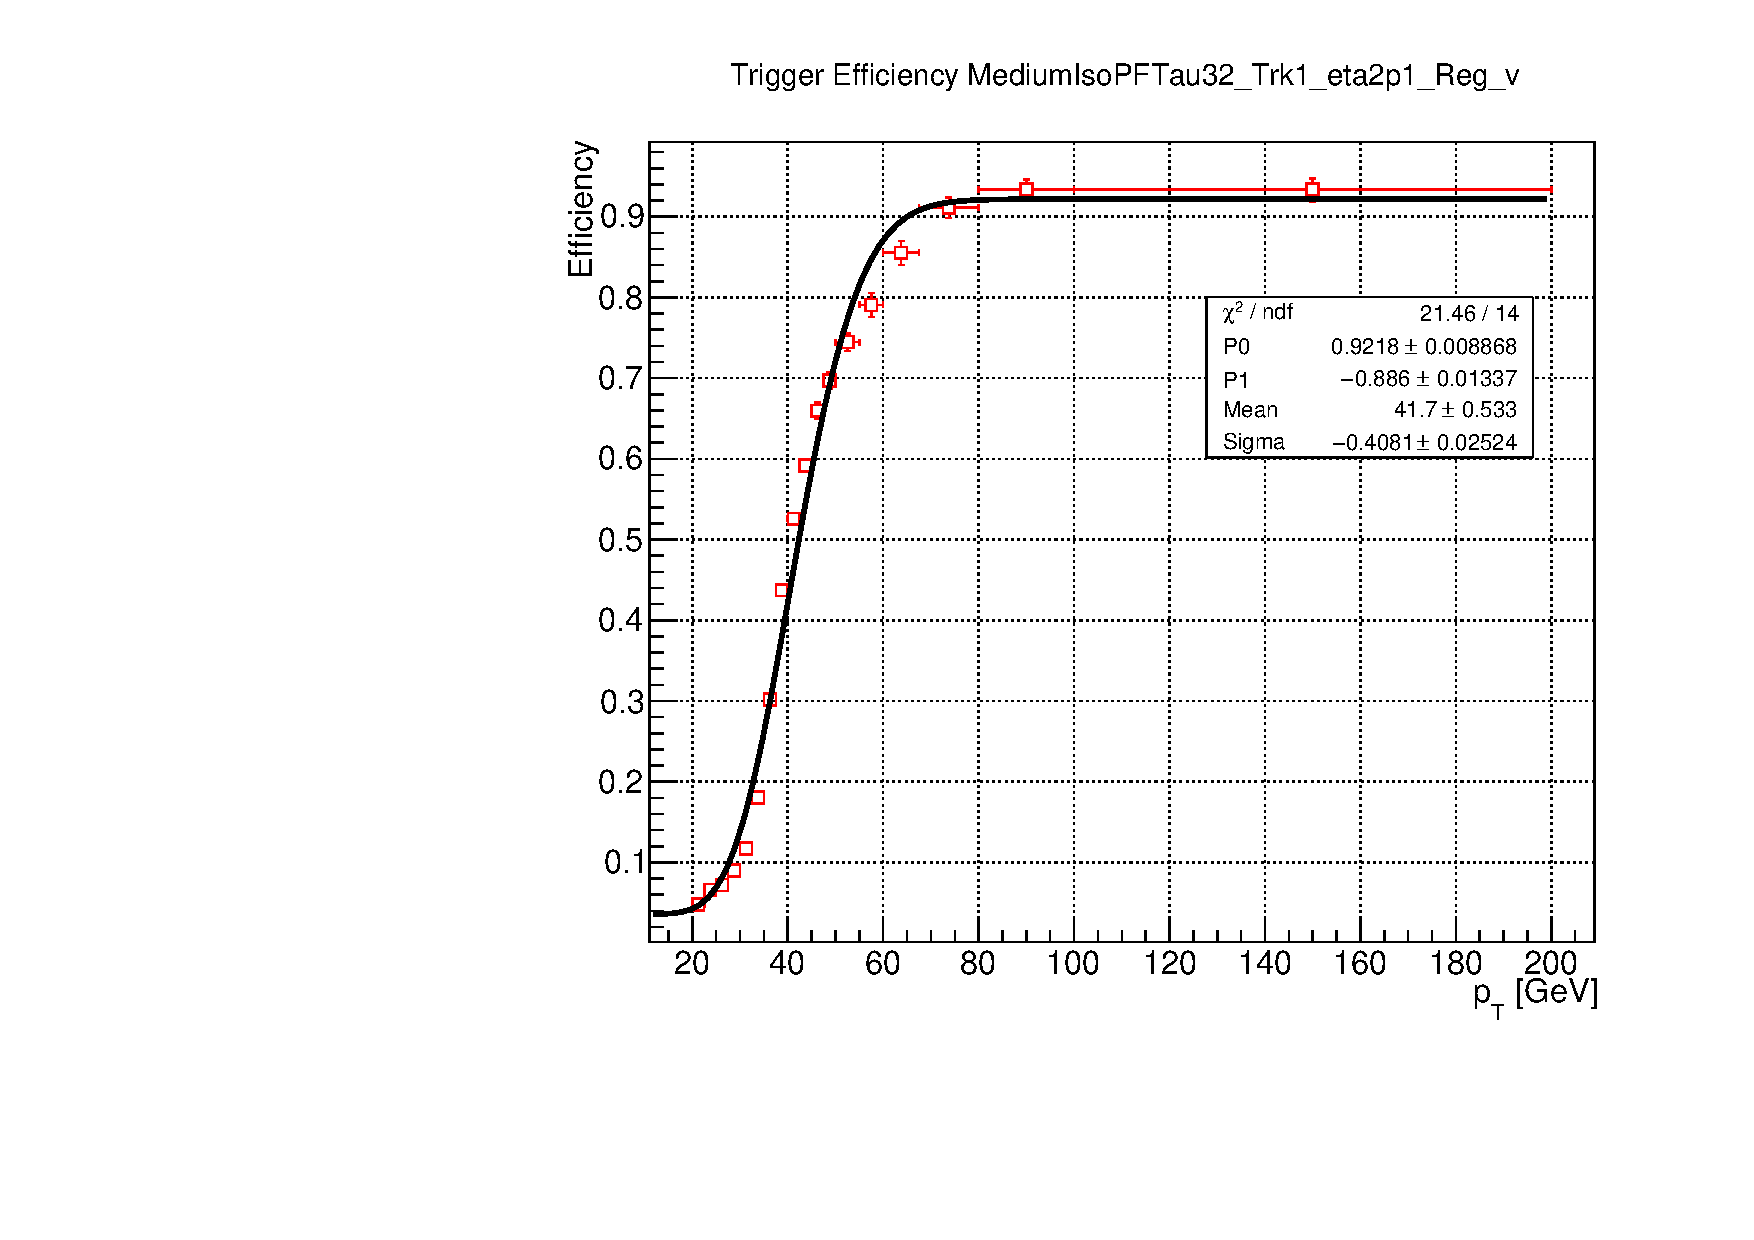
\includegraphics[clip,width=0.5\textwidth]{figuras/Chapter5/TriggerEff_mio.pdf}
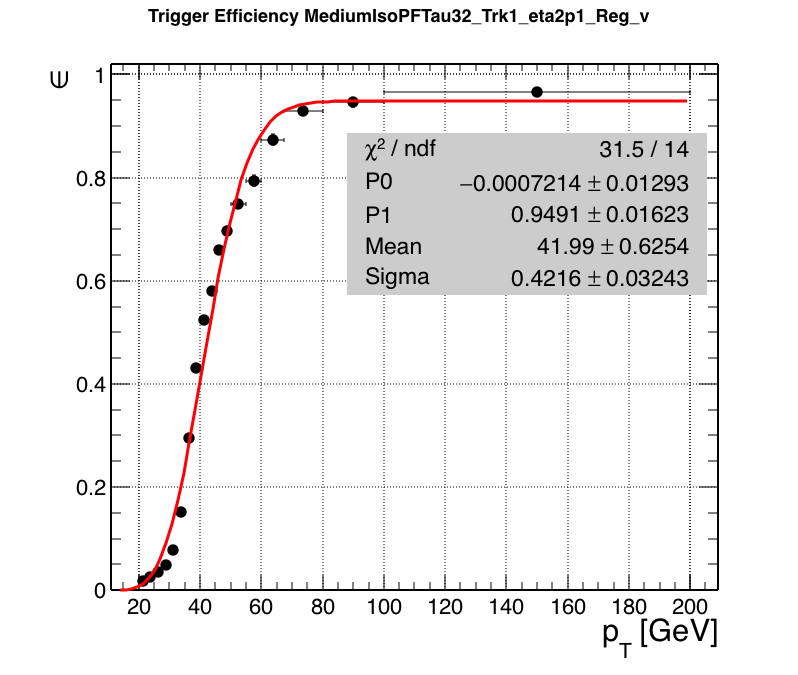
\includegraphics[clip,width=0.5\textwidth]{figuras/Chapter5/DiTauTriggerEfficiency_full_lumi.png}
 \caption{
  Trigger efficiency per \tauh~lepton as a function of \pt for data,
  obtained from the $Z \rightarrow \tau\tau \rightarrow \mu\tau_{h}$ events.
   }\label{fig:triggerEFf}
\end{center}
\end{figure}

\noindent The function used to perform the fit of the trigger efficiency curve is:
\begin{equation}
pdf=P[0]+P[1]\frac{1}{\sqrt{2\pi}}\int_{-\infty}^{y}e^{-\frac{t^{2}}{2}}dt \; ,
\end{equation}

\noindent where,

\begin{equation}
y=\frac{\sqrt{x}-\sqrt{P[2]}}{2P[3]}, \hspace{1cm} P[2]=\mu,\ P[3]=\sigma \; .
\end{equation}

\vspace{0.5cm}

\noindent The trigger weight applied per tau lepton is obtained from 
this fit.\\

\noindent In summary, the trigger selection is not applied on MC samples, instead, it
is modeled by weighting the MC predicted events. The weight, for each tau lepton, is 
obtained from the fit of the trigger efficiency curve from the 
data. Figure \ref{fig:triggerEFf} shows that the trigger efficiency reaches 
a plateau value of $\epsilon$=0.95 at tau-\pt~$=$70 \GeV. In consequence, in order to obtain
a well modeled trigger selection, and to avoid the turn-on curve, the hadronic taus must have 
transverse momenta greater than 70 \GeV.

\section{Data and Simulated samples}
\label{sec:Samples}

This section presents the data samples and  the MC samples
for signal and for background used in this analysis.

\subsection{Data Samples}
\label{subsec:Data}

This analysis uses the data collected by the CMS experiment
from the proton-proton collisions at 
\centermassenergy~of 13 \TeV~delivered by the LHC during 2016. The data 
recorded corresponds to a total integrated 
luminosity of 37.76 fb$^{-1}$ (Figure \ref{figchp2:luminosityRunII}, right). However, 
the data validated by the CMS Data Quality Monitoring team (CMSDQM) to be used 
for physics analyses has an integrated luminosity of 35.9 fb$^{-1}$. In order to guarantee 
that the right data is used, an official JSON file is issued containing all 
the ``good'' run ranges and lumi sections. The certified JSON file 
used in this analysis was:\\

\textit{Cert\_271036-284044\_13TeV\_03Feb2017ReReco\_Collisions16\_JSON.txt}. \\

\noindent For this thesis, the datasets, which include at least one triggered tau lepton at HLT
level, are shown in Table \ref{table:datasamples}. The trigger 
selection described in the previous section was applied to these datasets.

\begin{table}[h]
  \begin{center}
  \begin{tabular}{| l | c |}
  \hline\hline
        Physics Sample & Official CMS Datasets \\ [0.5ex] \hline \hline
        \footnotesize Run 2016B Tau Run2016B-03Feb2017  & \footnotesize \it /Tau/Run2016B-03Feb2017-v3/MINIAOD \\                                                                                                     
        \footnotesize Run 2016C Tau Run2016C-03Feb2017  & \footnotesize \it /Tau/Run2016C-03Feb2017-v1/MINIAOD \\                                                                                                     
        \footnotesize Run 2016D Tau Run2016D-03Feb2017  & \footnotesize \it /Tau/Run2016D-03Feb2017-v1/MINIAOD \\                                                                                                     
        \footnotesize Run 2016E Tau Run2016E-03Feb2017  & \footnotesize \it /Tau/Run2016E-03Feb2017-v1/MINIAOD \\                                                                                                     
        \footnotesize Run 2016F Tau Run2016F-03Feb2017  & \footnotesize \it /Tau/Run2016F-03Feb2017-v1/MINIAOD \\                                                                                                     
        \footnotesize Run 2016G Tau Run2016G-03Feb2017  & \footnotesize \it /Tau/Run2016G-03Feb2017-v1/MINIAOD \\                                                                                                     
        \footnotesize Run 2016Hv2 Tau Run2016H-03Feb2017& \footnotesize \it /Tau/Run2016H-03Feb2017\_ver2-v1/MINIAOD \\                                                                                               
        \footnotesize Run 2016Hv3 Tau Run2016H-03Feb2017& \footnotesize \it /Tau/Run2016H-03Feb2017\_ver3-v1/MINIAOD \\%\hline                                                                                        
  \hline                                                                                                                                                                                                              
  \hline                                                                                                                                                                                                              
  \end{tabular}                                                                                                                                                                                                       
  \end{center}
  \caption{Collision Data Samples}
  \label{table:datasamples} % is used to refer this table in the text                                                                                                                                                 
\end{table}

% The 
% CMSDQM selects the data with good quality according to the standard requirements that ensure the successful 
% data acquisition of all subdetectors. 

\subsection{Simulated Samples}
\label{subsec:Data}

The event simulation consists of two steps: the event 
generation simulates the particle production of a 
specific physics process; in the second step, the detector response 
is simulated. These processes are very complex and no analytical 
calculations can be performed therefore Monte Carlo (MC) techniques is used

% , instead, a probability is assigned 
% for an event to occur; in consequence, 
%  in order to describe, as accurate 
% as possible, such complex processes through numerical approaches. 


% the simulation of the interaction between 
% the particles and the detector material, where the observable final states 
% of the event are provided. 


\subsubsection{Event Simulation}
\label{subsubsec:eventSimulation}
%  The calculation of the production cross sections at 
%  the LHC for both interesting physics processes and their backgrounds relies 
%  upon a knowledge of the distribution of the momentum fraction x of the partons in a proton in 
%  the relevant kinematic range. 

\begin{itemize}
 \item \textbf{Event Generation:} \\
 The event generation is performed in four steps: the hard scattering, 
 the parton shower, the hadronization and the underlying event simulations.
 The hard scattering simulation consists of the calculation of the 
 probability amplitude for a specific physics process as a result of a pp-collision, using the 
 parton distribution functions (PDFs) and the matrix element (ME). A PDF is
 the probability density as a function of the momentum fraction carried 
 by a given parton. These functions are extracted from deep
 inelastic scattering data and from extrapolations to high energies. The ME 
 represents the probability amplitude of the process; its estimation
 depends on the level of the calculation performed. Event generations 
 usually includes Leading Order terms (LO) or 
 Next-to-Leading order terms (NLO), depending on the 
 availability of the calculations. Once the physics process of interest 
 is generated, then the subsequent hadronization processes are simulated
 models built to describe them. Finally, the underlying event is simulated
 depending on the energy and the processes from which it was produced. As a 
 result of the event generation, the four momentum of each particle
 emerging from the collision is produced. The most common generators used 
 are: \texttt{Phytia} \cite{bib:pythia}, \texttt{Madgraph} \cite{bib:madgraph}, 
 \texttt{POWHEG} \cite{bib:Powheg1,bib:Powheg2} 
 \texttt{Comphep} \cite{bib:comphep}, \texttt{Sherpa} \cite{bib:sherpa}, among 
 others. \texttt{Pythia} is widely used due to the accurate modeling of parton shower production
and fragmentation, while \texttt{POWHEG} has a very accurate description of processes
like top quark decay and \texttt{Madgraph} is very precise describing SM processes like Drell-Yan. \\

 %  
%  , which are the dominant at such 
%  energy scales, 
%  are simulated considering phenomenological 

 
  \item \textbf{Detector Response Simulation:}\\
  The second step is the simulation of particles passing through the 
  detector. In order to describe such interactions, a detailed 
  modeled of the CMS geometry is needed. The 
  software must be able to accurately describe the effects of magnetic 
  field, the electromagnetic and hadronic shower production, and so on. For 
  this purpose, the CMS Collaboration uses the package 
  \texttt{GEANT4} \cite{bib:geant4,bib:FullSim}. As a result
  all the observable final states produced from the pp collision, as their 
  kinematic measured variables, are given.\\
\end{itemize}

\noindent The whole event simulation results into a RAW data file, which has the same 
format as the one delivered by the HLT system with real 
data. Then, the simulated events are reconstructed, following the data processing 
described in Section \ref{chap2:dataprocessing}. \\

\subsubsection{Signal and Background MC Samples}
\label{subsubsec:MCSamples}

\noindent The CMS collaboration issues official MC samples for all the 
Standard Model processes to be used in physics analyses. In this thesis, the official 
$Spring\_miniAODv2\_2016$ MC samples were used. The signal samples of 
the \Zprime~production, as well as the samples for the SM processes, described in section \ref{sec:Bkg},
were generated  using \texttt{Pythia8}, \texttt{Madgraph-v5}, and \texttt{POWHEG}, where 
the tau lepton decays were simulated with a specialized package called \texttt{TAUOLA} \cite{bib:tauola}.
The detector simulation was perform using \texttt{GEANT4}. \\
% \begin{tiny} %%TABLE MC SAMPLES

\noindent The background MC samples used in this thesis are shown in Table \ref{tab:mc_samples}. The 
production of the Drell-Yan and QCD MC samples was performed using the next-to-leading order
\texttt{Madgraph-v5} generator (NLO$\_$MG5), while the same generator was used 
for the W+Jets background but with the leading order version (LO$\_$MG5). The 
\texttt{Pythia8} generator was used for the production of Di-Boson background, while 
the \texttt{POWHEG} generator was used for the $t\bar{t}$ background. \\

\noindent The Drell-Yan MC samples were binned using the mass of the generated lepton pair, while the QCD and W+Jets MC samples 
were binned using $H_{T}$ \footnote{$H_{T}$, the transverse hadronic energy, is defined as the scalar sum of the
transverse momenta of the jet constituents.}.\\

\begin{table}[H]
  \begin{center}
%  \centering{
   \begin{tabular}{| l | l | c | r |}
  \hline\hline
        \scriptsize Process &\scriptsize samples &\scriptsize MC generator &\scriptsize cross-section (pb) \\ [-0.5ex] \hline

    \footnotesize $Z \to ll $   &\scriptsize  $m >$ 50 \GeV~                  &\scriptsize NLO$\_$MG5 &\scriptsize  5765.4000\\
    \scriptsize mass binned     &\scriptsize  200 \GeV~ $< m <$ 400 \GeV~     &\scriptsize NLO$\_$MG5 &\scriptsize  7.9077\\
    \scriptsize NLO samples     &\scriptsize  400 \GeV~ $< m <$ 500 \GeV~     &\scriptsize NLO$\_$MG5 &\scriptsize  0.4263  \\
                                &\scriptsize  500 \GeV~ $< m <$ 700 \GeV~     &\scriptsize NLO$\_$MG5 &\scriptsize  0.2390  \\
                                &\scriptsize  700 \GeV~ $< m <$ 800 \GeV~     &\scriptsize NLO$\_$MG5 &\scriptsize  0.0341  \\
                                &\scriptsize  800 \GeV~ $< m <$ 1000 \GeV~    &\scriptsize NLO$\_$MG5 &\scriptsize  0.0288  \\
                                &\scriptsize  1000 \GeV~ $< m <$ 1500 \GeV~   &\scriptsize NLO$\_$MG5 &\scriptsize  0.0150  \\
                                &\scriptsize  1500 \GeV~ $< m <$ 2000 \GeV~   &\scriptsize NLO$\_$MG5 &\scriptsize  0.0018  \\
                                &\scriptsize  2000 \GeV~ $< m <$ 3000 \GeV~   &\scriptsize NLO$\_$MG5 &\scriptsize  0.0004  \\
    \hline                                                                                                                                                                                                                                                       
    \footnotesize $W + jets $   &\scriptsize  0 \GeV~ $< HT <$ 70 \GeV~       &\scriptsize LO$\_$MG5 &\scriptsize   61526.508 \\ 
    \scriptsize HT binned                   &\scriptsize  70 \GeV~ $< HT <$ 100 \GeV~     &\scriptsize LO$\_$MG5 &\scriptsize   1600.976  \\
    \scriptsize LO samples                  &\scriptsize  100 \GeV~ $< HT <$ 200 \GeV~    &\scriptsize LO$\_$MG5 &\scriptsize   1632.534  \\
                                &\scriptsize  200 \GeV~ $< HT <$ 400 \GeV~    &\scriptsize LO$\_$MG5 &\scriptsize   436.597   \\
                                &\scriptsize  400 \GeV~ $< HT <$ 600 \GeV~    &\scriptsize LO$\_$MG5 &\scriptsize   59.366    \\
                                &\scriptsize  600 \GeV~ $< HT <$ 800 \GeV~    &\scriptsize LO$\_$MG5 &\scriptsize   14.626    \\
                                &\scriptsize  800 \GeV~ $< HT <$ 1200 \GeV~   &\scriptsize LO$\_$MG5 &\scriptsize   6.677     \\
                                &\scriptsize  1200 \GeV~ $< HT <$ 2500 \GeV~  &\scriptsize LO$\_$MG5 &\scriptsize   1.613     \\
                                &\scriptsize  2500 \GeV~ $< HT <$ Inf         &\scriptsize LO$\_$MG5 &\scriptsize   0.039     \\
    \hline
    \footnotesize $t \overline{t}$   &\scriptsize                             &\scriptsize POWHEG    &\scriptsize  831.76     \\
    \hline
    
    \footnotesize Di-Boson      &\scriptsize  $WW$       &\scriptsize PYTHIA8   &\scriptsize   63.21 \\ 
                                &\scriptsize  $WZ$       &\scriptsize PYTHIA8   &\scriptsize   22.82 \\ 
                                &\scriptsize  $ZZ$       &\scriptsize PYTHIA8   &\scriptsize   10.32 \\ 
    \hline                                                                                                                                                                                                                                                       
    \footnotesize QCD           &\scriptsize  50 \GeV~  $< HT <$ 100 \GeV~     &\scriptsize NLO$\_$MG5 &\scriptsize   246700000.0 \\ 
    \scriptsize HT binned                   &\scriptsize  100 \GeV~ $< HT <$ 200 \GeV~     &\scriptsize NLO$\_$MG5 &\scriptsize    28080000.0  \\
    \scriptsize NLO samples                  &\scriptsize  200 \GeV~ $< HT <$ 300 \GeV~     &\scriptsize NLO$\_$MG5 &\scriptsize     1712000.0  \\
                                &\scriptsize  300 \GeV~ $< HT <$ 500 \GeV~     &\scriptsize NLO$\_$MG5 &\scriptsize      347500.0   \\
                                &\scriptsize  500 \GeV~ $< HT <$ 700 \GeV~     &\scriptsize NLO$\_$MG5 &\scriptsize       32100.0    \\
                                &\scriptsize  700 \GeV~ $< HT <$ 1000 \GeV~    &\scriptsize NLO$\_$MG5 &\scriptsize        6823.0    \\
                                &\scriptsize  1000 \GeV~ $< HT <$ 1500 \GeV~   &\scriptsize NLO$\_$MG5 &\scriptsize        1208.0     \\
                                &\scriptsize  1500 \GeV~ $< HT <$ 2000 \GeV~   &\scriptsize NLO$\_$MG5 &\scriptsize         120.0     \\
                                &\scriptsize  2000 \GeV~ $< HT <$ Inf          &\scriptsize NLO$\_$MG5 &\scriptsize          25.3     \\
  \hline                                                                                                                                                                                                                                                         
  \hline                                                                                                                                                                                                                                                         
  \end{tabular}                                                                                                                                   
  \end{center}
  \caption{MC Samples used for this analysis.}
%   }
  \label{tab:mc_samples}
\end{table}
% \end{tiny}


\noindent Similar to the background, the signal samples are simulated using \texttt{Pythia8}, and the 
tau decays are simulated using \texttt{TAUOLA}. The signal samples for different \Zprime~mass values, using 
the SSM, are shown in Table \ref{tab:signal_samples}.

\section{Event Selection}
\label{sec:EventSelection}

In the previous sections, the datasets presented in the previous were passed 
through the \\ $HLT\_DoubleMediumIsoPFTau35\_Trk1\_eta2p1$ trigger
(see section \ref{sec:TriggerSelection}). An additional selection of events 
was performed with these data, with the purpose to identify the \Zprimetotauh~signature; this selection 
was split in two categories: the \tauh~identification and the topological selections.

\begin{table}[H] %% TABLE SIGNAL POINTS
  \begin{center}
  \begin{tabular}{| l | c | r | r |}
  \hline\hline
       \scriptsize Process (mass point [\GeV])                 &\scriptsize  MC generator  &\scriptsize width[\GeV] &\scriptsize cross-section (pb) \\ [0.5ex] \hline

    \footnotesize $\text{SSM}~$\Zprime~$ (500)$    &\scriptsize  PYTHIA8       &\scriptsize 14.73    &\scriptsize 5.75100      \\             
%     \footnotesize $\text{SSM}~$\Zprime~$ (750)$    &\scriptsize  PYTHIA8       &\scriptsize 22.89    &\scriptsize 1.23600      \\    
    \footnotesize $\text{SSM}~$\Zprime~$ (1000)$   &\scriptsize  PYTHIA8       &\scriptsize 30.97    &\scriptsize 0.38650     \\  
%     \footnotesize $\text{SSM}~$\Zprime~$ (1250)$   &\scriptsize  PYTHIA8       &\scriptsize 39.02    &\scriptsize 0.14900      \\
    \footnotesize $\text{SSM}~$\Zprime~$ (1500)$   &\scriptsize  PYTHIA8       &\scriptsize 47.05    &\scriptsize 0.06479    \\
    \footnotesize $\text{SSM}~$\Zprime~$ (1750)$   &\scriptsize  PYTHIA8       &\scriptsize 55.07    &\scriptsize 0.03104    \\
    \footnotesize $\text{SSM}~$\Zprime~$ (2000)$   &\scriptsize  PYTHIA8       &\scriptsize 63.10    &\scriptsize 0.01583    \\
    \footnotesize $\text{SSM}~$\Zprime~$ (2500)$   &\scriptsize  PYTHIA8       &\scriptsize 79.16    &\scriptsize 0.00468   \\
    \footnotesize $\text{SSM}~$\Zprime~$ (3000)$   &\scriptsize  PYTHIA8       &\scriptsize 95.24    &\scriptsize 0.00159   \\
    \footnotesize $\text{SSM}~$\Zprime~$ (3500)$   &\scriptsize  PYTHIA8       &\scriptsize 111.30    &\scriptsize 0.00059  \\
%     \footnotesize $\text{SSM}~$\Zprime~$ (4000)$   &\scriptsize  PYTHIA8       &\scriptsize 127.50    &\scriptsize 0.00024  \\
  \hline                                                                                                                                                                                                                                                         
  \hline                                                                                                                                                                                                                                                         
  \end{tabular}                                                                                                                                                                                                                                                  
  \end{center}
  \caption{MC Signal Samples with Production Campaign: RunIISummer16MiniAODv2-PUMoriond17\_80X\_mcRun2\_asymptotic\_2016\_TrancheIV\_v6-v1}
  \label{tab:signal_samples}
\end{table}

\subsection{$\tau_{h}$~Identification}
\label{subsec:TauSelection}

\noindent In this analysis the hadronic taus were reconstructed 
using the HPS algorithm, seeded by jets reconstructed with 
the anti-kT algorithm and whose transverse momenta are higher 
than 30 \GeV. Additionally, discriminators are applied 
in order to distinguish the \tauh~signature from those produced by
QCD jets, electrons, and muons (see Section \ref{subsec:TauIdentification}).
The \tauh-identification is crucial to reduce the QCD jet background, 
which is the dominant SM contamination of the \Zprimetotauh~sample. \\

\noindent Events were required to have taus with 1or3-prongs, whose decay mode 
is reconstructed using the \textit{newDMF} discriminator. We used 1or3-prongs selection
since it represents 95$\%$ of the hadronic tau decays; additionally,
the unphysical 2-prong decay mode was not included, since it produced
a decrease on the sensitivity of the analysis (Appendix \ref{chap:TauIDStudies}). 
Figure \ref{ntracks} shows the n-prongs for the leading $\tau$ after all tau requirements.
On the other hand, the selection of the \textit{newDMF} discriminator was motivated by the agreement between 
the data and the level of background extracted from a control region dominated by the Drell-Yan;
this control region, used to validate the background simulation samples, will be described in
see Section \ref{subsec:DY}. The comparison with the other discriminator (\textit{oldDMF}) is 
presented  in Appendix \ref{chap:TauIDStudies}.  \\

\noindent Taus are required to have a transverse momentum greater than 70 \GeV~for two reasons:
first, this high \pt~cut allows to reduce the QCD-contamination, which is expected 
to be considerable at low-\pt~values; second, because for this \pt~range, a 
constant 95$\%$ trigger efficiency is 
obtained (see Section \ref{sec:TriggerSelection}). Figure \ref{ptdistributions}
shows the \pt~distributions for the leading tau and the second tau,
after applying the tau identification requirements. These taus are also required 
to be in the pseudorapidity region of $|\eta| < 2.1$, due to the high efficiency 
of charged-particle track reconstruction in the barrel 
region (see Figure \ref{fig:Track_Efficiencies}), which is not only crucial 
for the tau reconstruction but also for the tau isolation. This pseudorapidity
range is covered by the single tau L1-trigger acceptance. Figure \ref{etadistributions} shows the 
$\eta$~distributions for the leading tau and the second tau, after requiring the tau identification criteria;
note that the background is spread over all $\eta$-range, while the $\eta$-distribution for the signal 
is centered at $\eta = 0$.\\
% because its production comes from the hard interaction.\\

\begin{figure}[H]
 \begin{center}
 \captionsetup[subfloat]{farskip=0pt,captionskip=0.0cm,labelformat=empty}
 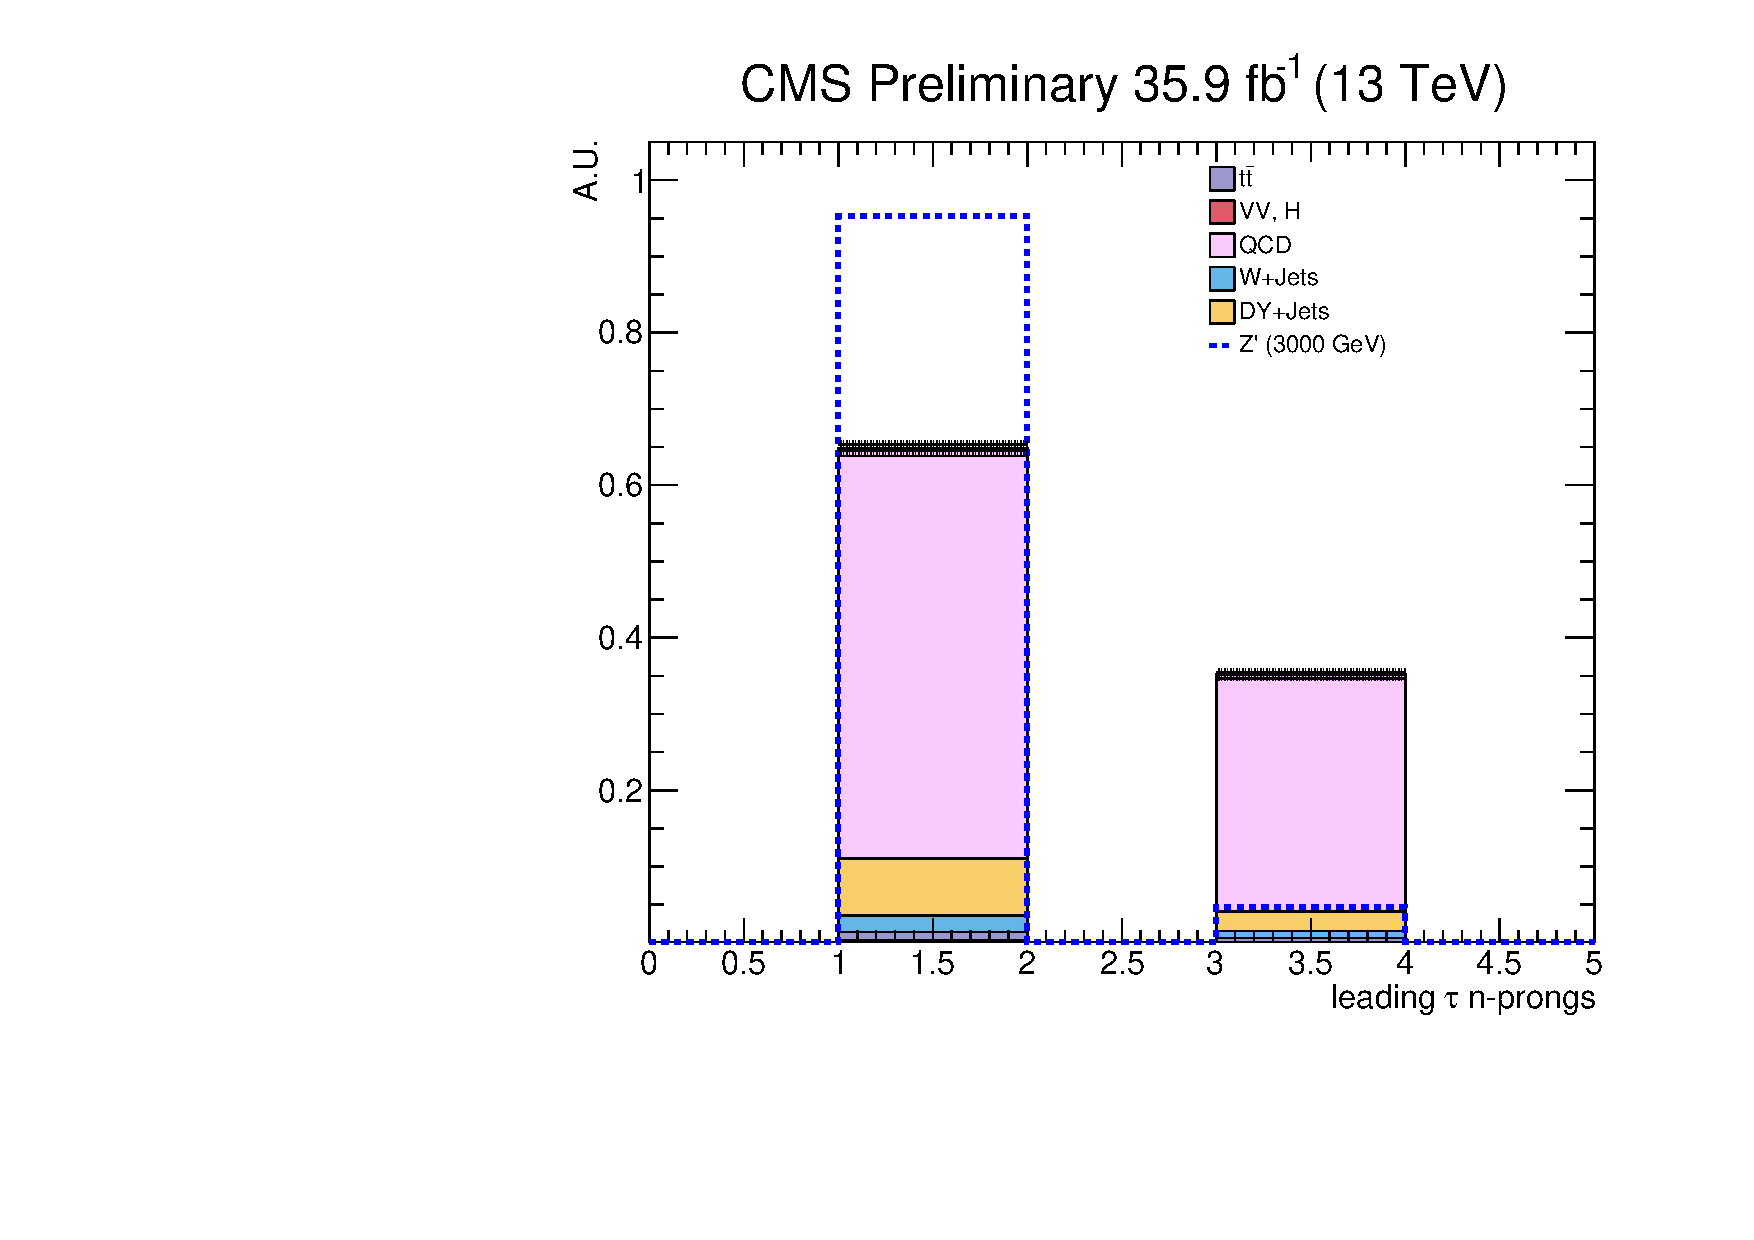
\includegraphics[clip,width=0.43\textwidth]{figuras/Chapter5/TauID_Plots/nTracks.pdf}
 \end{center}
 \caption{n-prong distribution, normalized to unity, for the leading tau after all tau requirements. QCD was estimated via data-driven method (see Section \ref{subsec:QCD})}
 \label{ntracks}
 \end{figure}

 \begin{figure}[H]
 \begin{center}
 \captionsetup[subfloat]{farskip=0pt,captionskip=0.0cm,labelformat=empty}
 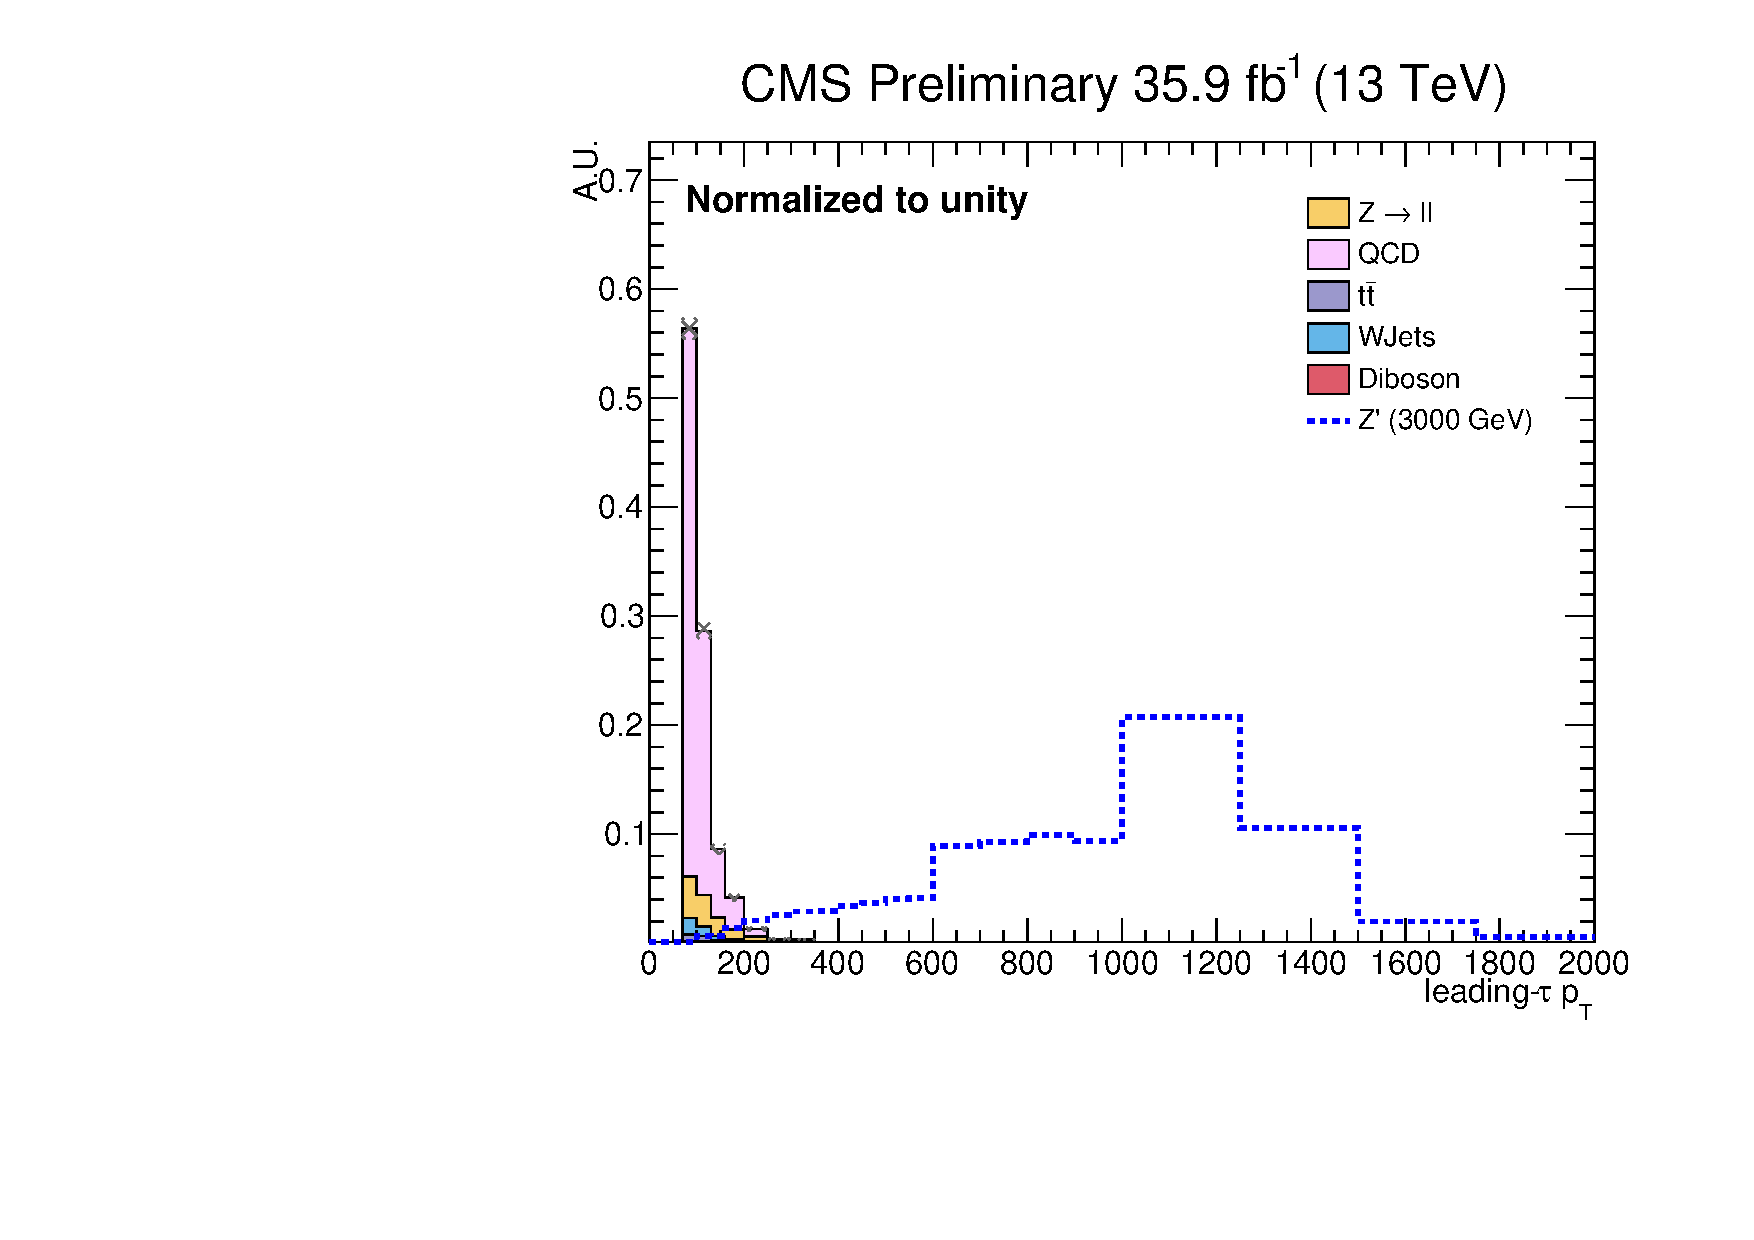
\includegraphics[clip,width=0.43\textwidth]{figuras/Chapter5/TauID_Plots/leadingtaupt.pdf}
  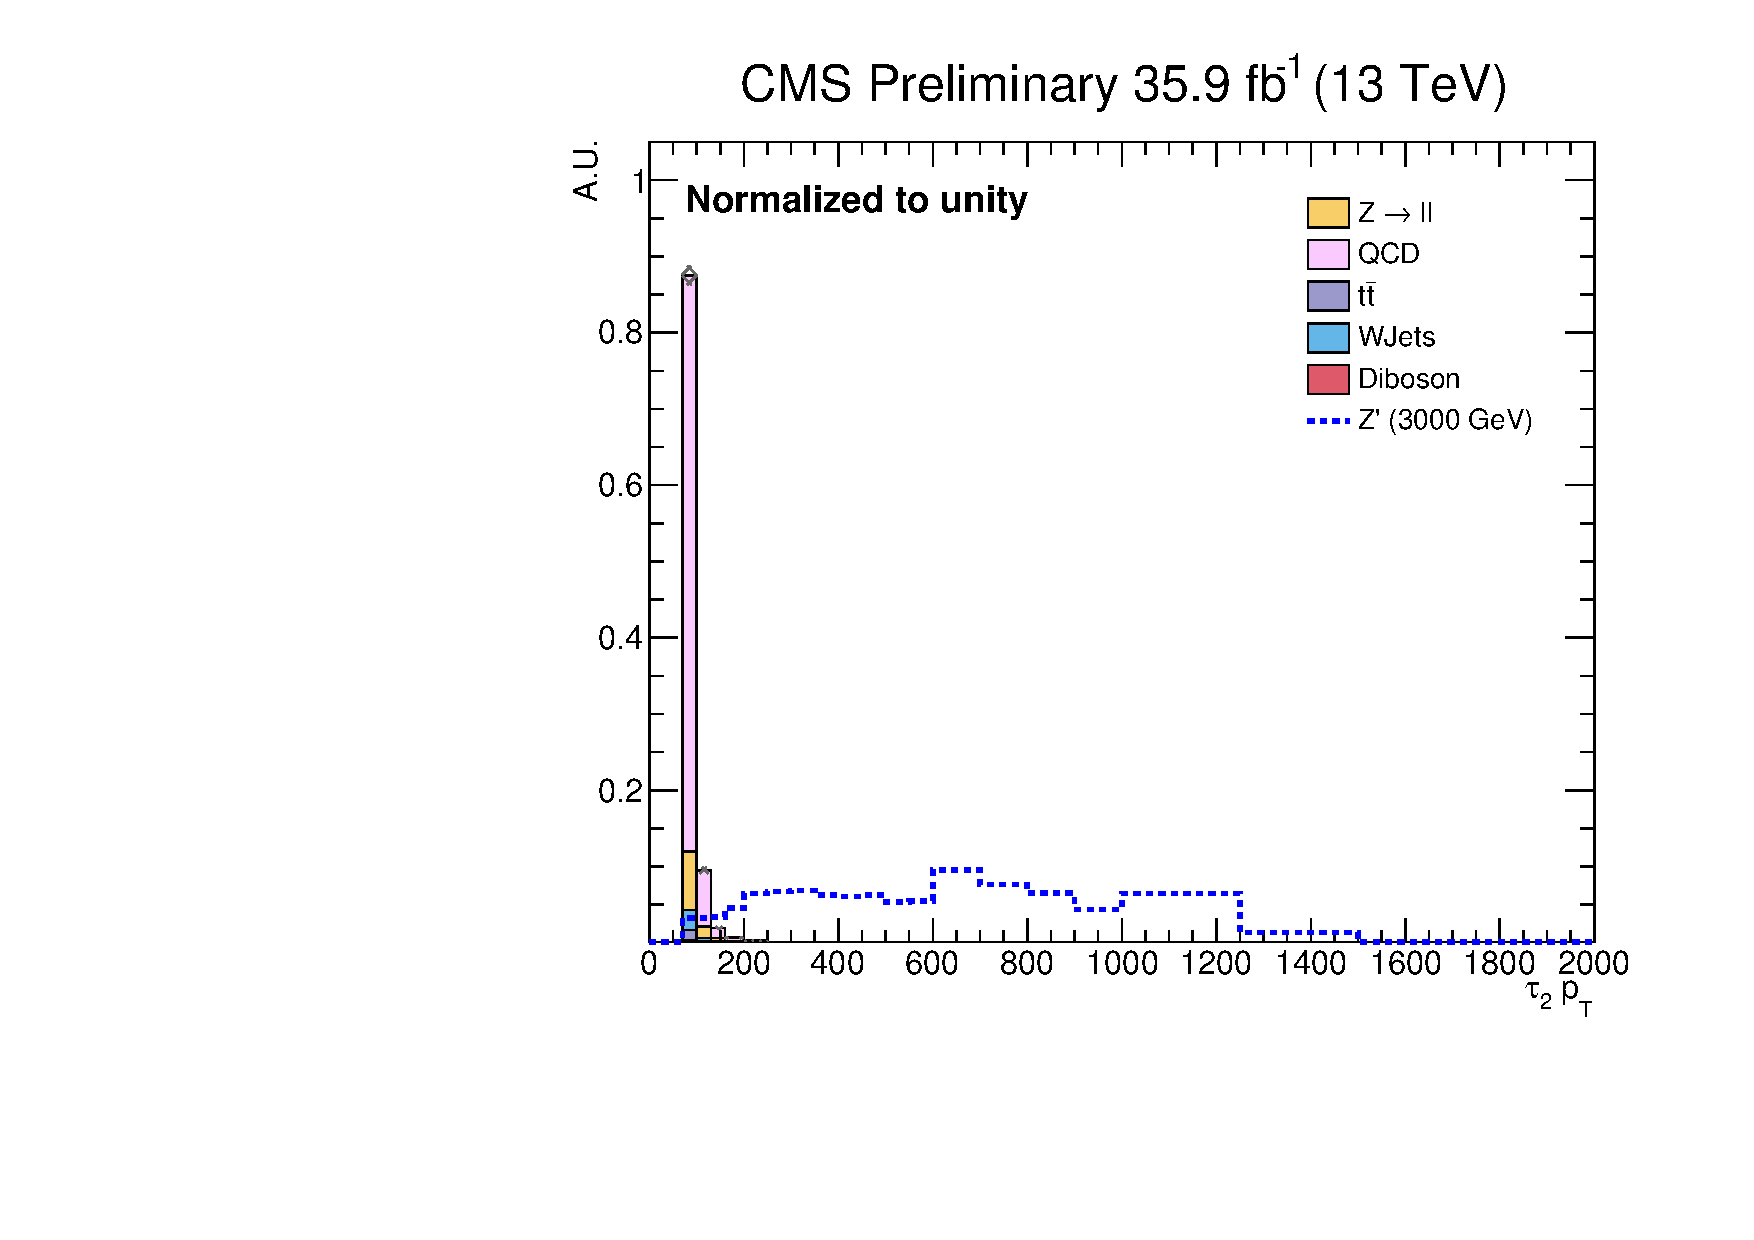
\includegraphics[clip,width=0.43\textwidth]{figuras/Chapter5/TauID_Plots/tau2pt.pdf}
 \end{center}
 \caption{\pt~distributions, normalized to unity, for the leading tau (right) and the second tau (left), after all tau requirements. QCD was estimated via data-driven method (see Section \ref{subsec:QCD})}
 \label{ptdistributions}
 \end{figure}
 
 
\noindent In order to distinguish the \tauh~candidate from QCD-jets, the 
\textit{tight} WP of the MVA-based isolation discriminator was 
required (\textit{byTightIsolationMVArun2v1DBnewDMwLT}); this WP ensures
a $\tau$~identification efficiency of $\sim$60$\%$ and a QCD jet rejection 
rate of $\sim$99.8$\%$. For the discrimination against electrons, 
a \textit{loose} WP was required (\textit{againstElectronMVALooseMVA6}) in order to 
keep a high tau reconstruction efficiency (85$\%$) and a relatively
low fake rate ($10 ^{-2}$). Additionally, the \tauh~candidates are required
to pass the \textit{tight} WP of the against-muons 
cutoff-based discriminator (\textit{againstMuonTight3}), whose 
tau identification efficiency is more than 99$\%$, while the misidentification 
probability is 1.4 $\times 10^{-3}$. The impact on the sensitivity due 
to the WP of the discriminators against QCD-jets, electrons and muons is presented in 
Appendix \ref{chap:TauIDStudies}. The \tauh~identification criteria, used in this 
analysis, is summarized in Table \ref{tab:tauID}.\\

\begin{figure}[H]
 \begin{center}
 \captionsetup[subfloat]{farskip=0pt,captionskip=0.0cm,labelformat=empty}
 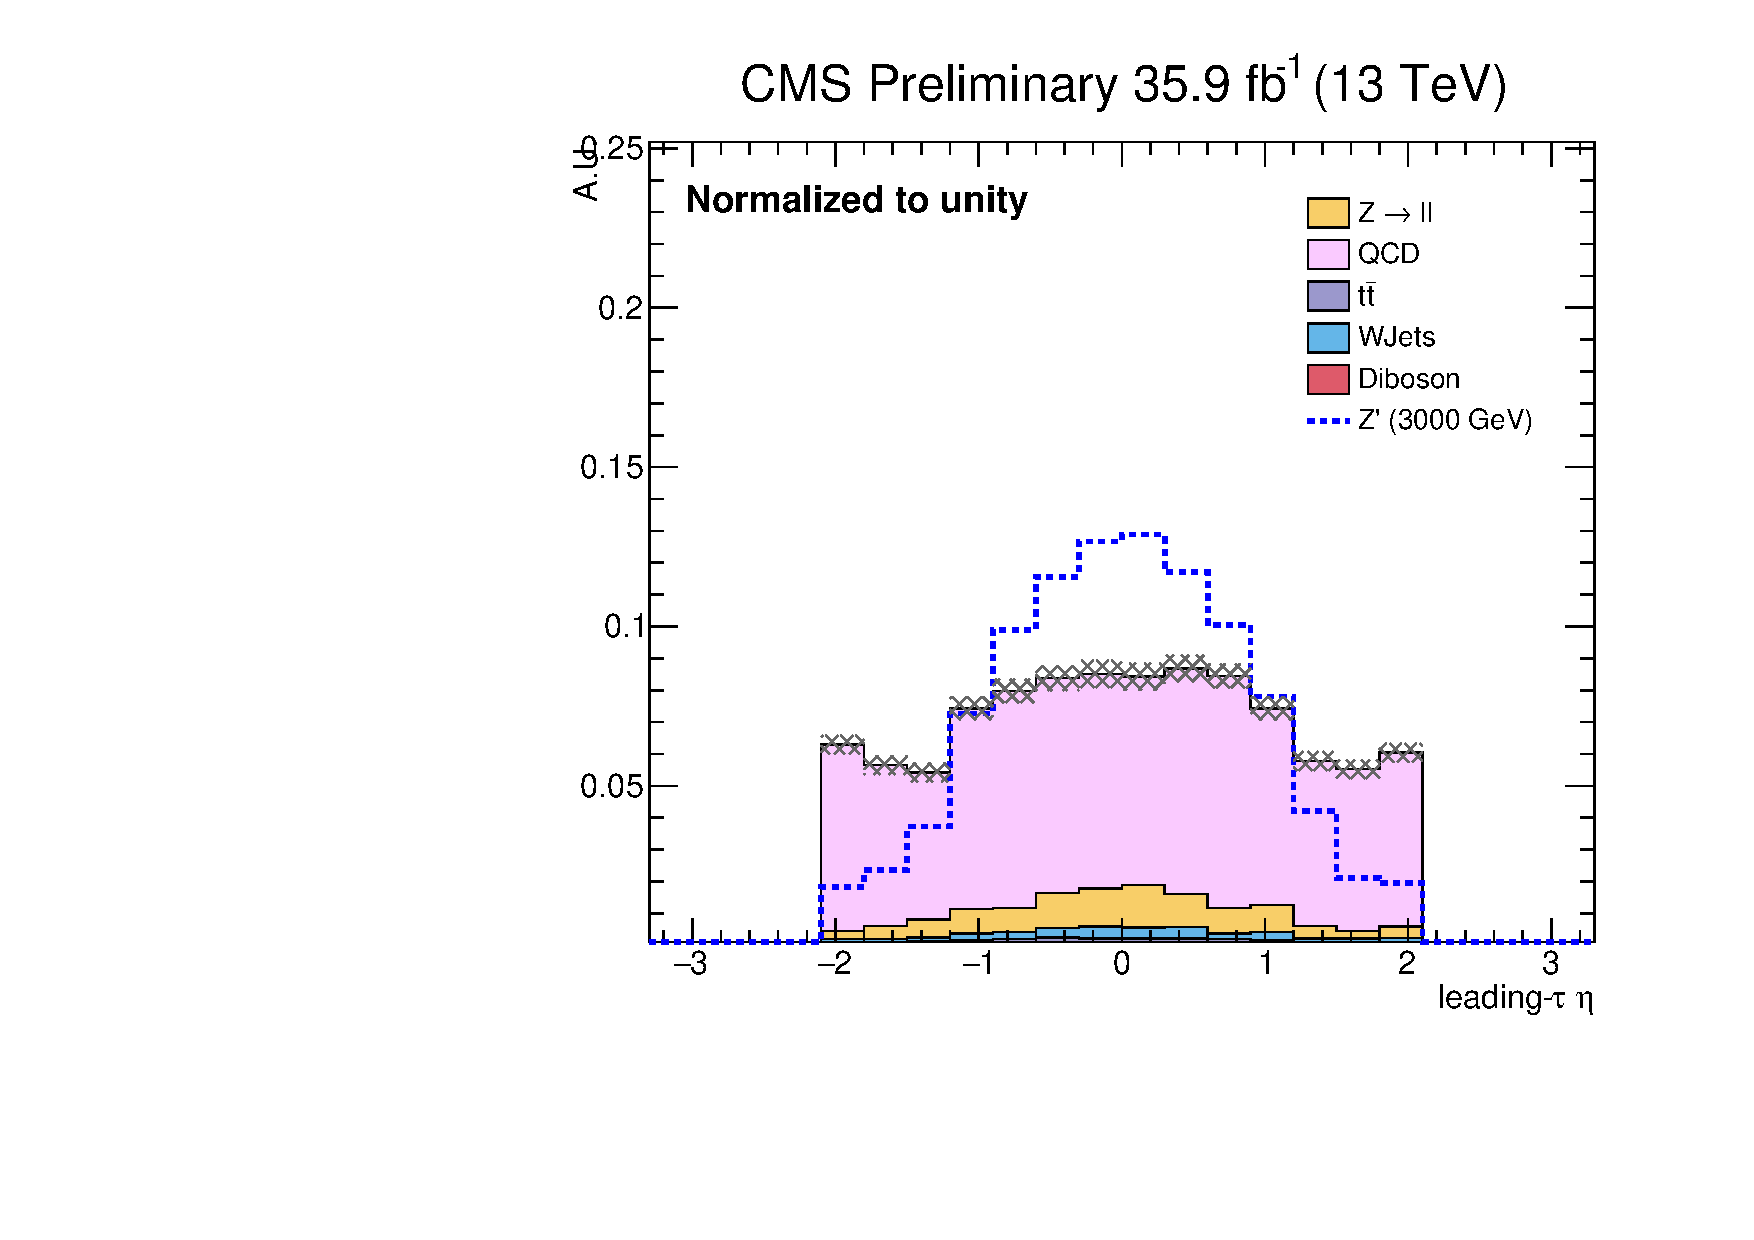
\includegraphics[clip,width=0.43\textwidth]{figuras/Chapter5/TauID_Plots/leadingtaueta.pdf}
  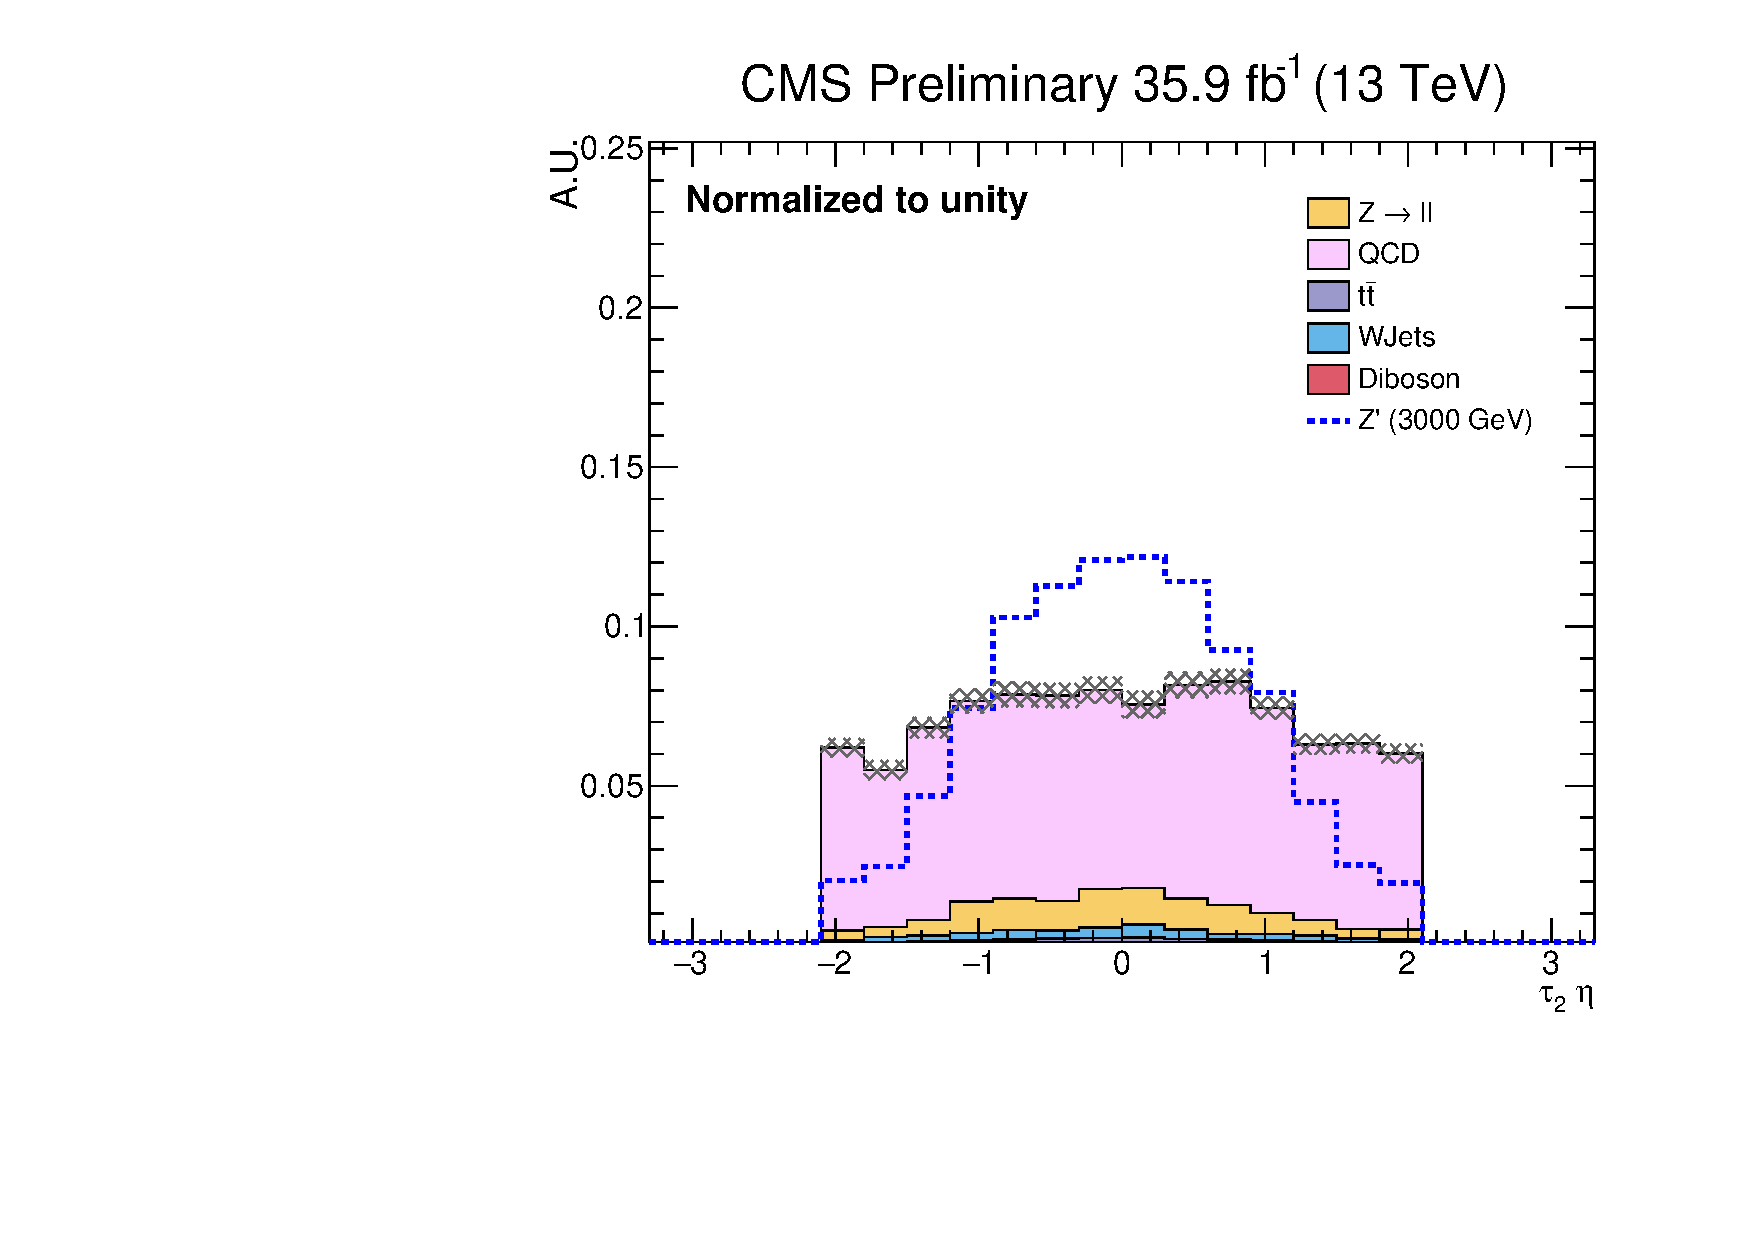
\includegraphics[clip,width=0.43\textwidth]{figuras/Chapter5/TauID_Plots/tau2eta.pdf}
 \end{center}
 \caption{$\eta$~distributions, normalized to unity, for the leading tau (right) and the second tau (left), after all tau requirements. QCD was estimated via data-driven method (see Section \ref{subsec:QCD})}
 \label{etadistributions}
 \end{figure}


\begin{table}[H]
    \begin{center}
    \begin{tabular}{l|l} \hline \hline 
 \pt                    &  $>$  70 \GeV \\
 $|\eta|$               &  $<$ 2.1 \\
 Tau Decay               & \textit{1or3-prongs} \\
                        & \textit{newDMF} \\
 Isolation Disc.        & \textit{byTightIsolationMVArun2v1DBnewDMwLT} \\
 Anti-electron Disc.    & \textit{againstElectronMVALooseMVA6} \\
 Anti-muon Disc.        & \textit{againstMuonTight3} \\ \hline \hline 
  \end{tabular}
  \end{center}
  \caption{Tau Identification Criteria}
  \label{tab:tauID}
\end{table}

% \noindent The impact of the \tauh~identification criteria on 
% the sensitivity was studied.  Besides, 

\subsection{Topological Selections}
\label{subsec:TopologicalSelections}
% , considering that its signature was discussed in 
% the previous Chapter (see Section \ref{sec:Signal}). 

%  The selection criteria based on the topology 
% of the \Zprimetotauh~events are presented in this section. 

\noindent Since the \Zprime~boson is expected to 
be massive, the two oppositely-charged taus would be moving 
in opposite directions. Therefore, the $\Delta R (\tau_{1},\tau_{2}) > 0.3$
requirement is applied to ensure that the hadronic tau pair is well 
separated in the $\eta-\phi$ plane. As can be seen in Figure \ref{DeltaRdistribution},
the \DRt~distribution for the signal is centered around $\pi$, which is a manifestation of
the back-to-back production of the taus, as expected. \\

% in the transverse plane in
% a $\eta$~average close to zero.\\

\noindent Additionally, as was mentioned in Section \ref{sec:Signal}, due to presence of neutrinos,
a missing transverse energy (\MET) is expected in the signal events. Figure \ref{MET}
shows the \MET~distribution after applying the tau identification criteria. As can be seen in the 
figure, an \MET~cut will reduce considerably the QCD contamination. A requirement of 
\MET~above 30 \GeV~will reduce the QCD background by 57$\%$, while it keeps
94$\%$ of the signal yield. Additionally, this cut allows to reduce the 
W+Jets contamination by 27$\%$, since no momentum imbalance is expected for 
this background. As will be discussed in Section \ref{subsec:QCD}, this cut 
is also motivated by the fact that the \MET~$<$ 30 \GeV~region is highly 
contaminated by QCD events, which can be exploited to estimate this background. \\
%Even more, since there is a high QCD expected 

\begin{figure}[H]
 \begin{center}
 \captionsetup[subfloat]{farskip=0pt,captionskip=0.0cm,labelformat=empty}
 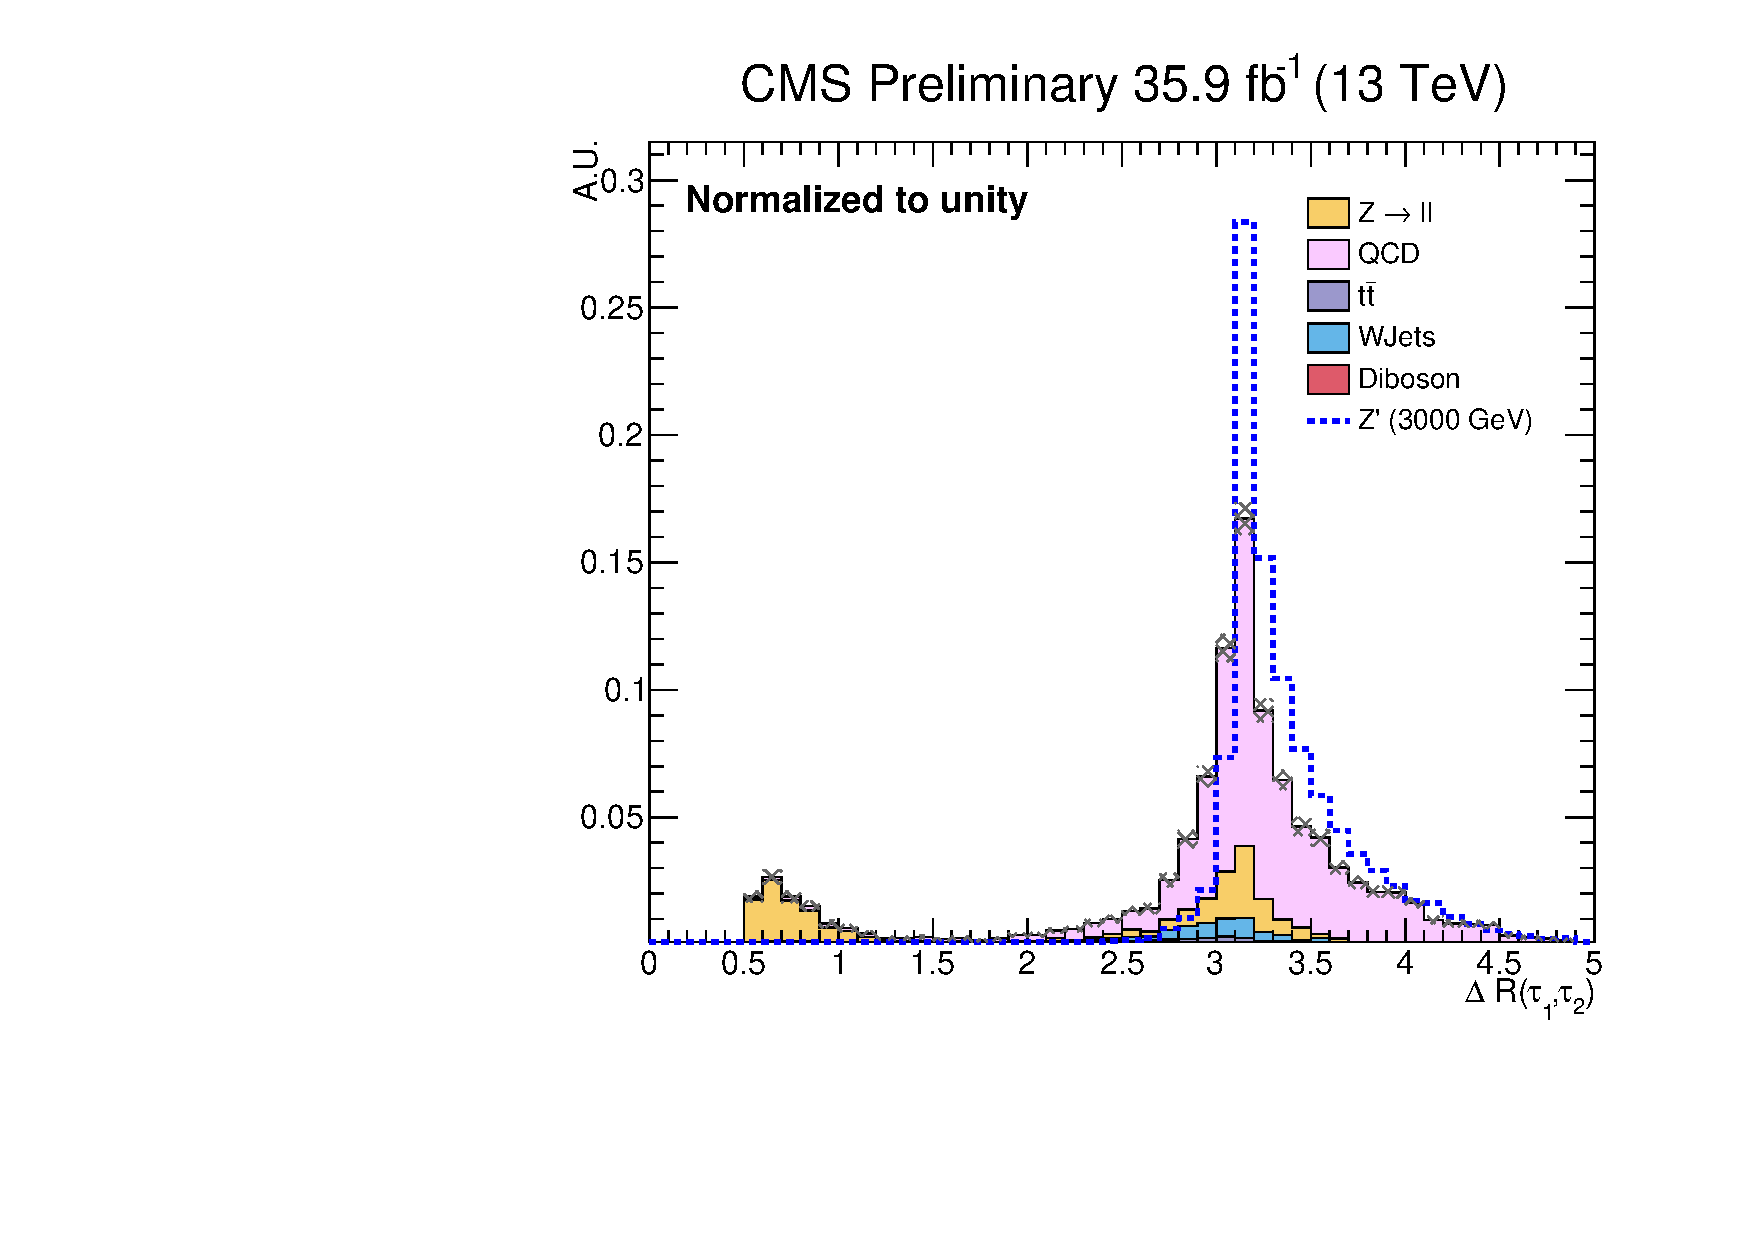
\includegraphics[clip,width=0.43\textwidth]{figuras/Chapter5/TauID_Plots/DeltaR.pdf}
 \end{center}
 \caption{\DRt~distribution, normalized to unity, for the di-tau pair after all tau identification requirements. QCD was estimated 
 via data-driven method (see Section \ref{subsec:QCD}).}
 \label{DeltaRdistribution}
 \end{figure}


 \begin{figure}[H]
 \begin{center}
 \captionsetup[subfloat]{farskip=0pt,captionskip=0.0cm,labelformat=empty}
 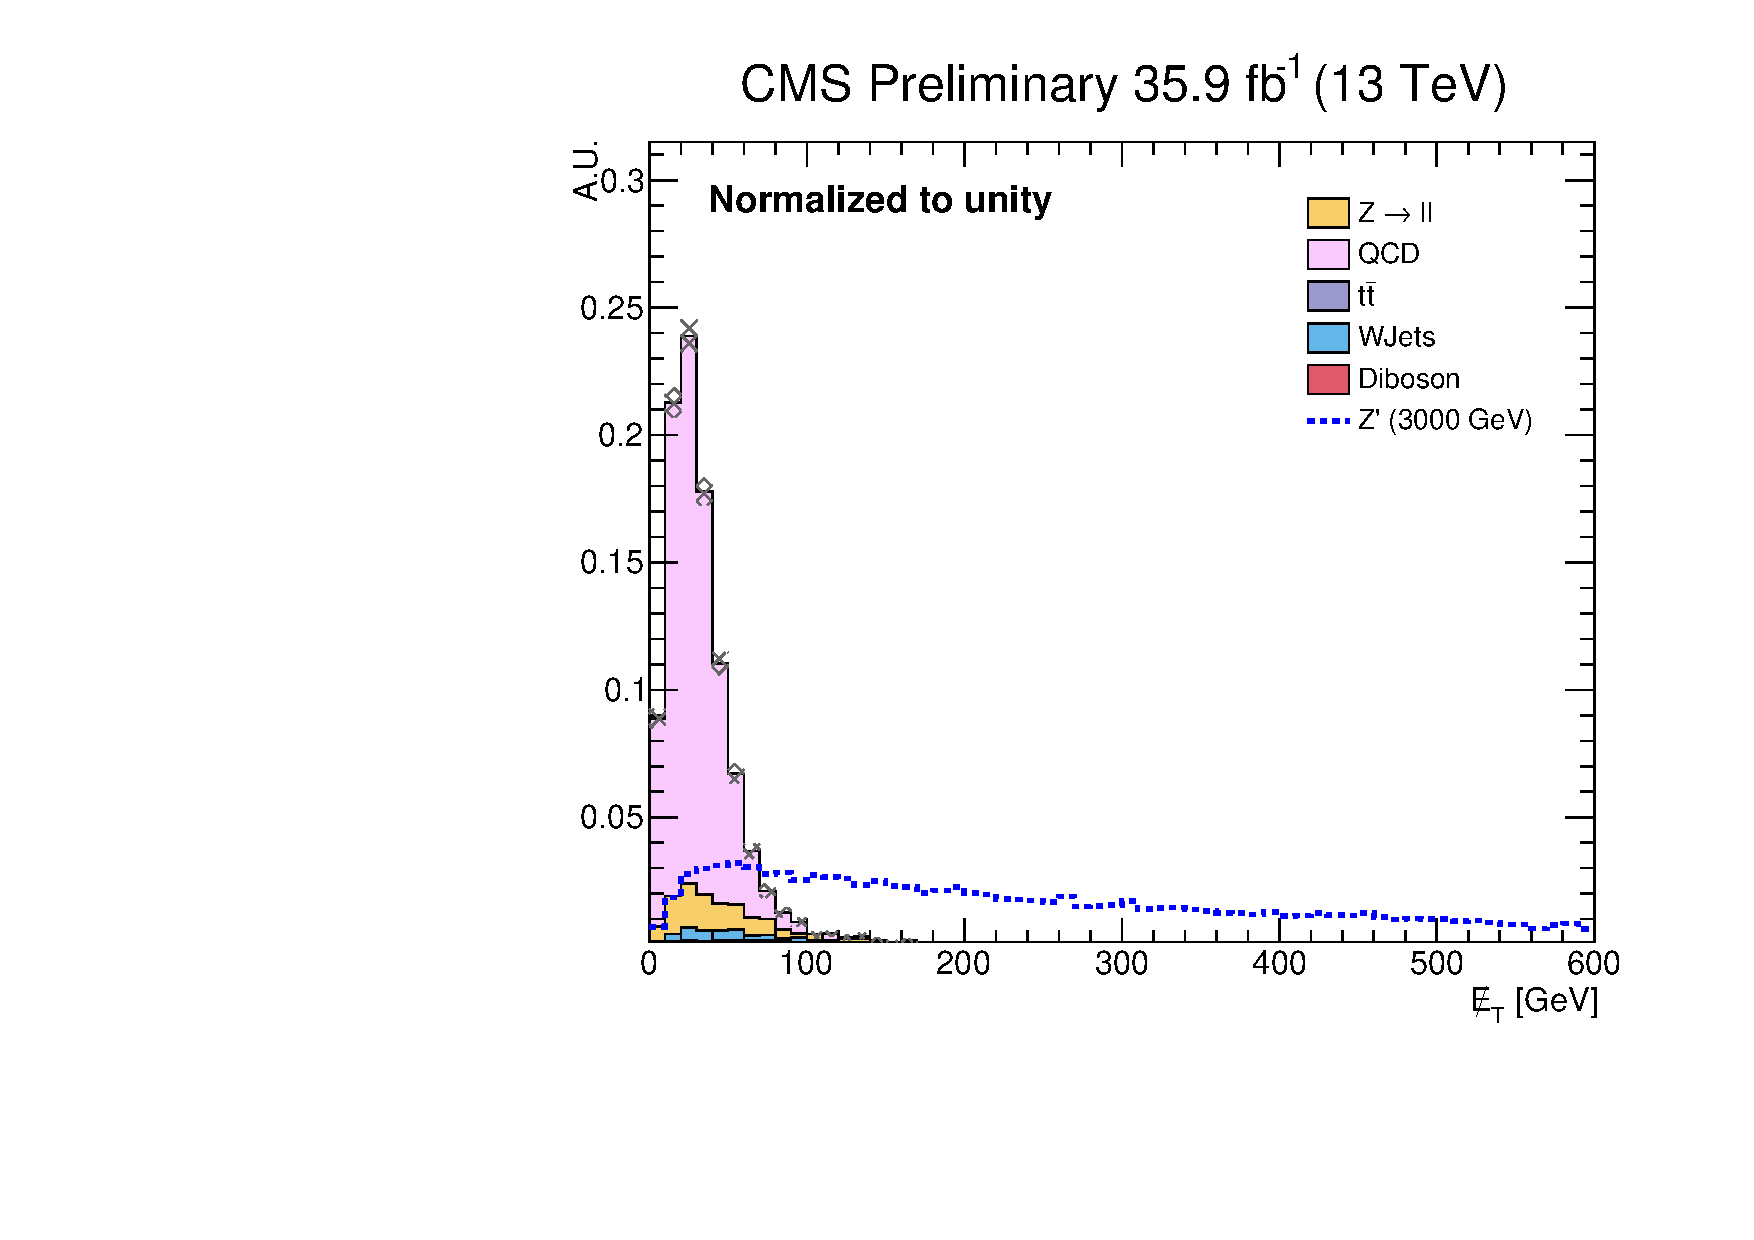
\includegraphics[clip,width=0.43\textwidth]{figuras/Chapter5/TauID_Plots/MET.pdf}
 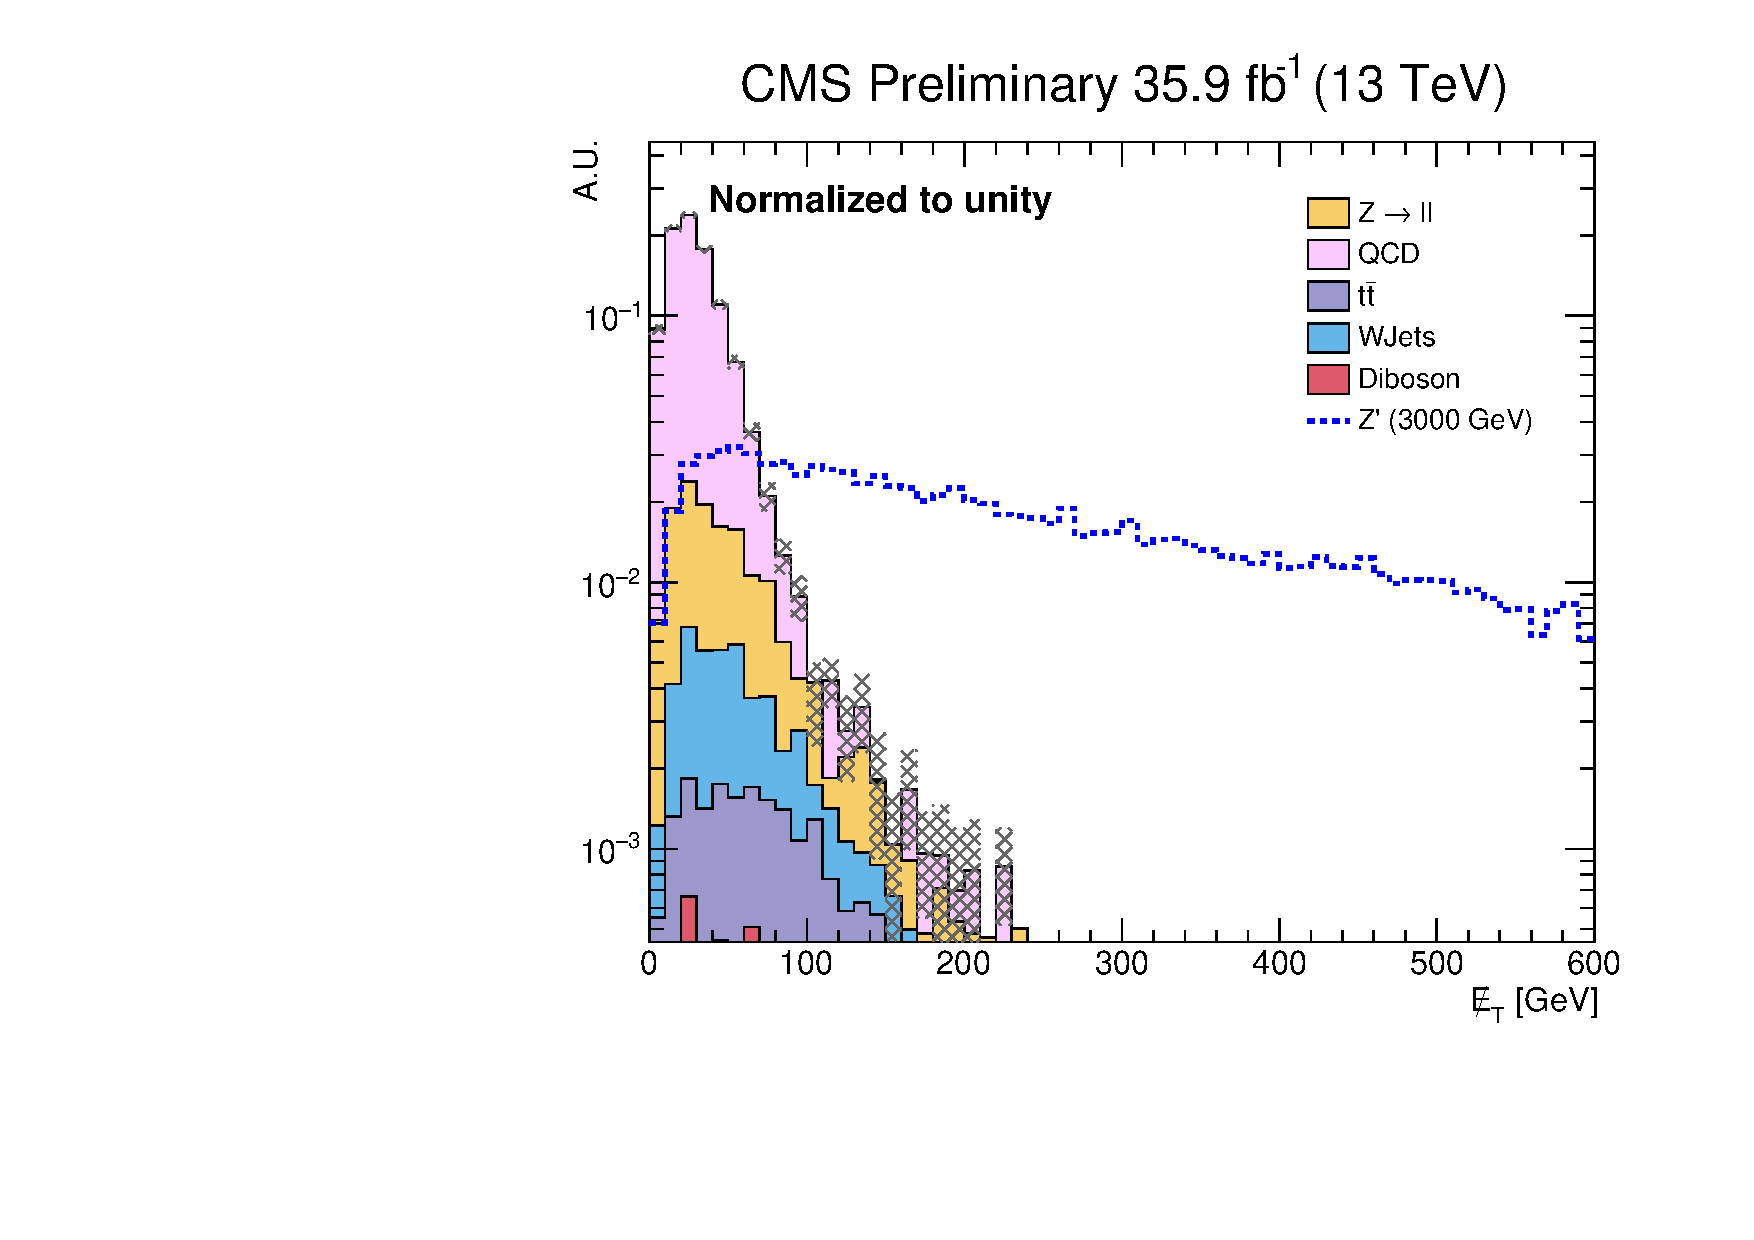
\includegraphics[clip,width=0.43\textwidth]{figuras/Chapter5/TauID_Plots/MET_log.pdf}
 \end{center}
 \caption{\MET~distribution, normalized to unity, in linear (left) and log (right) scale after all tau identification requirements. QCD was estimated 
 via data-driven method (see Section \ref{subsec:QCD}).}
 \label{MET}
 \end{figure}

\noindent The b-jet signature can fake the one produced by a high-\pt~tau and, in consequence,
a b-jet veto is applied on the events. The veto is applied to any jet
tagged as b-jet using the \textit{loose} WP of the CSVv2 algorithm, which provides 
a reconstruction efficiency of 83$\%$ (See Section \ref{sec:bJet}). This veto allows to reduce 
the $t\bar{t}$ background since, as mentioned in Section \ref{sec:Bkg}, 
the top quark most of the times decays into a bottom quark. The b-jet veto
reduces by 74$\%$ the $t\bar{t}$ background, while the signal efficiency 
is kept at 90$\%$. Figure \ref{bjet} shows the distribution of the number of b-jets 
after requiring the tau identification criteria and the \MET~cut.\\

  \begin{figure}[H]
 \begin{center}
 \captionsetup[subfloat]{farskip=0pt,captionskip=0.0cm,labelformat=empty}
 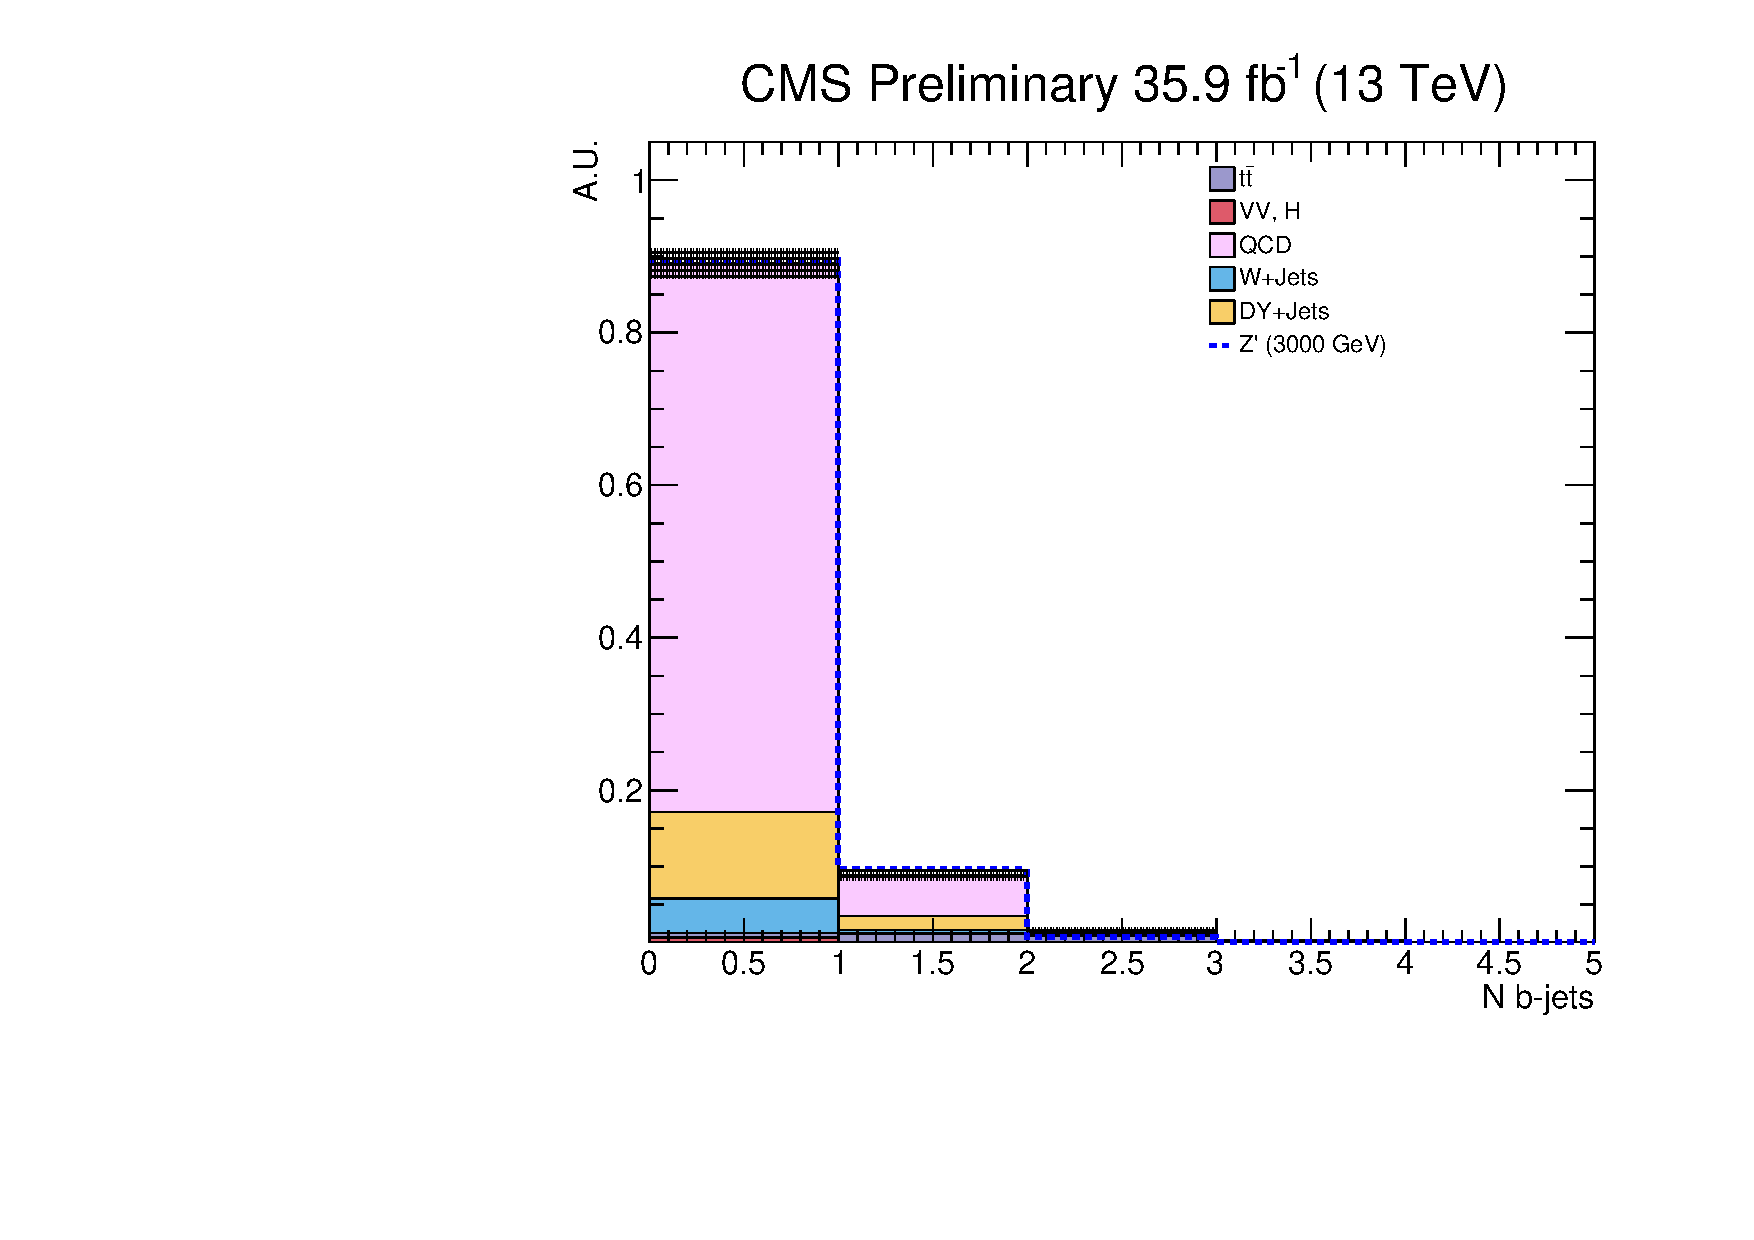
\includegraphics[clip,width=0.43\textwidth]{figuras/Chapter5/TauID_Plots/NBJets.pdf}
 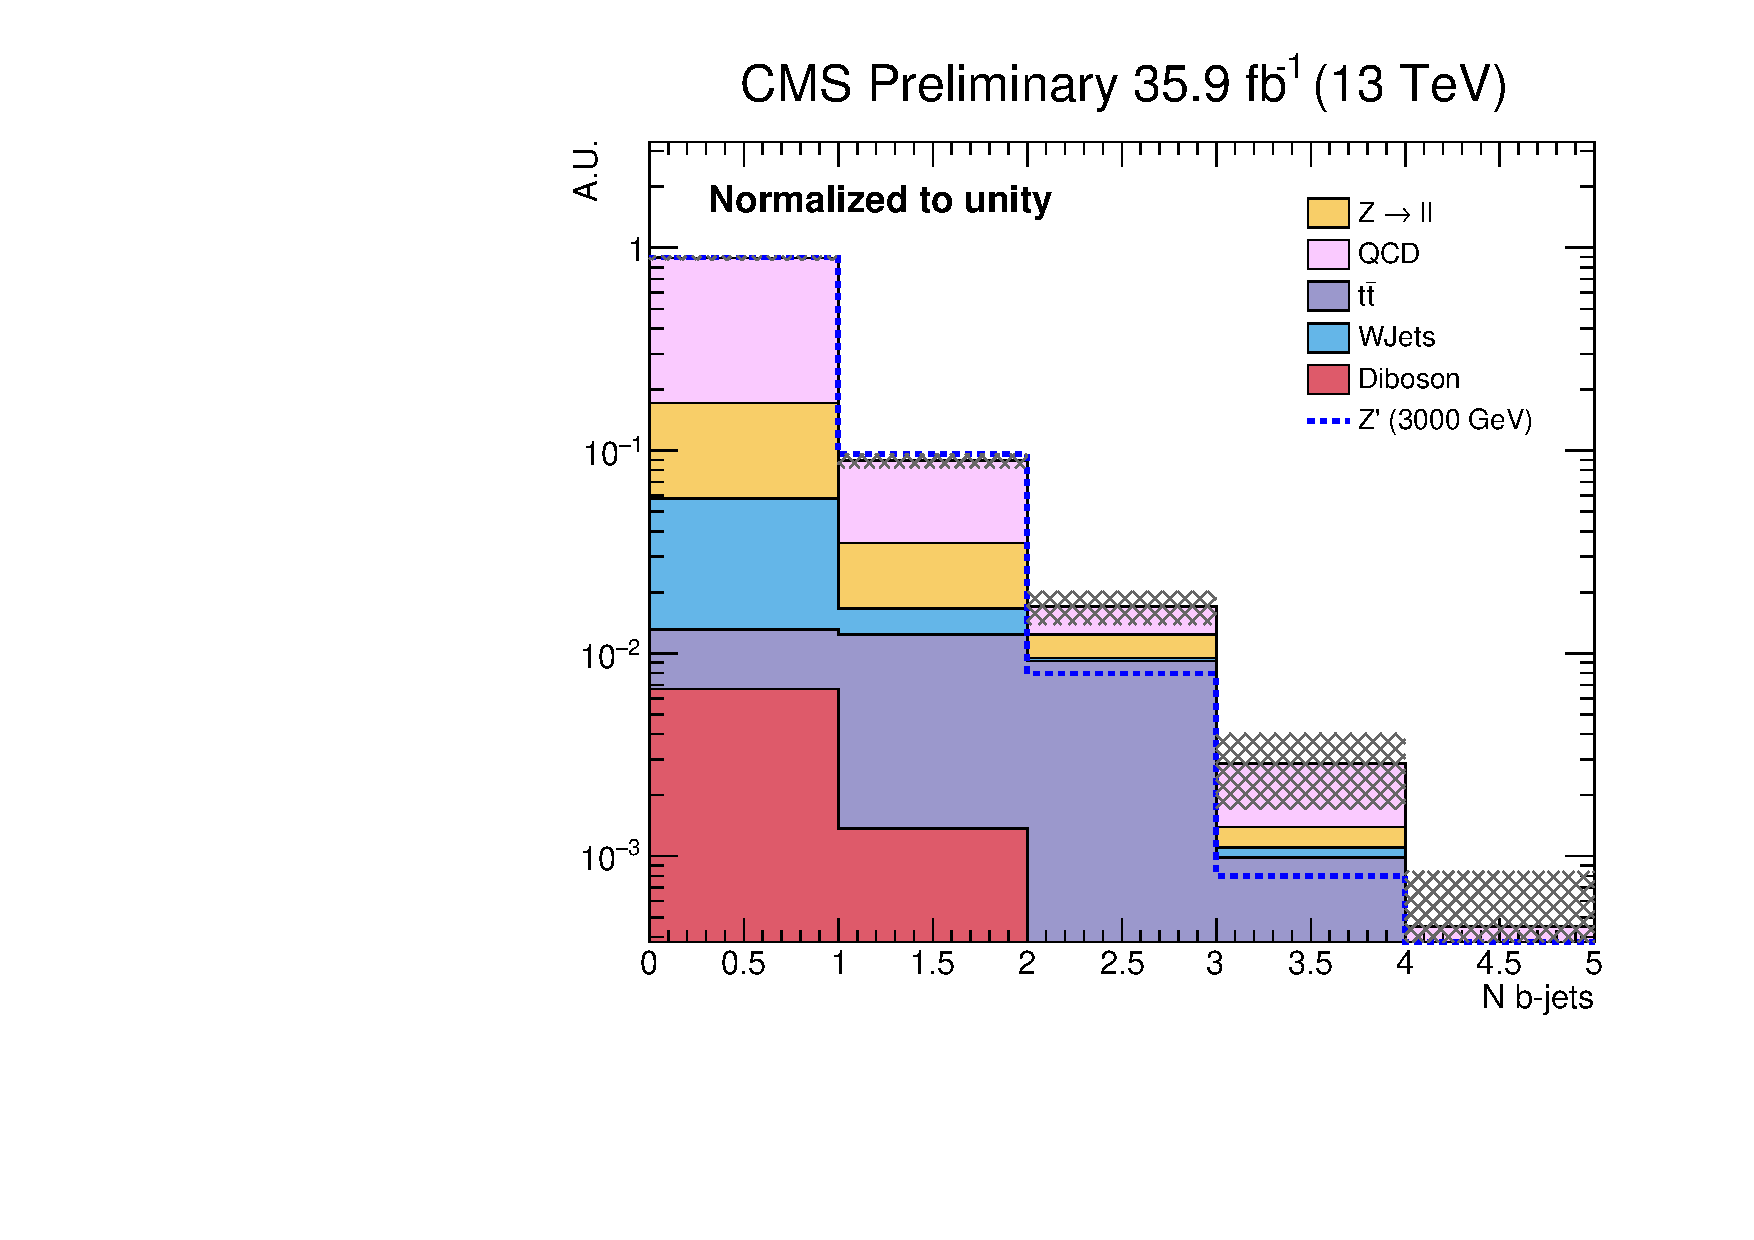
\includegraphics[clip,width=0.43\textwidth]{figuras/Chapter5/TauID_Plots/NBJets_log.pdf}
 \end{center}
 \caption{Distribution of number of jets tagged as b-jets, normalized to unity, in linear (left) and log (right) scale, after 
 the tau identification and \MET~requirements. QCD was estimated  via data-driven method (see Section \ref{subsec:QCD}).}
 \label{bjet}
 \end{figure}

 \noindent Since both taus coming from the \Zprime~decay are expected to be back-to-back
 in the transverse plane, the $\cos\Delta \phi (\tau_{1},\tau_{2}) < -0.95$ cut is required in 
 the events. Figure \ref{cosDphi} shows the $\cos\Delta \phi (\tau_{1},\tau_{2})$ distribution after applying
 the tau identification, the \MET, and the b-jet veto cuts. Since the production of the 
 two taus is uncorrelated for the QCD and W+Jets backgrounds, this requirement
 reduces those backgrounds by 58$\%$ and 24$\%$, respectively, while 
 81$\%$ of the signal events are kept. \\
 
%  the  move back-to-back by random they are reduced, respectively, 58$\%$ and 24$\%$ by this cut, 
%  , while the QCD and W+Jets background, where the two taus are moving back-to-back by random, are reduced 58$\%$ and 24$\%$,
%  respectively. \\
 
  \begin{figure}[H]
 \begin{center}
 \captionsetup[subfloat]{farskip=0pt,captionskip=0.0cm,labelformat=empty}
 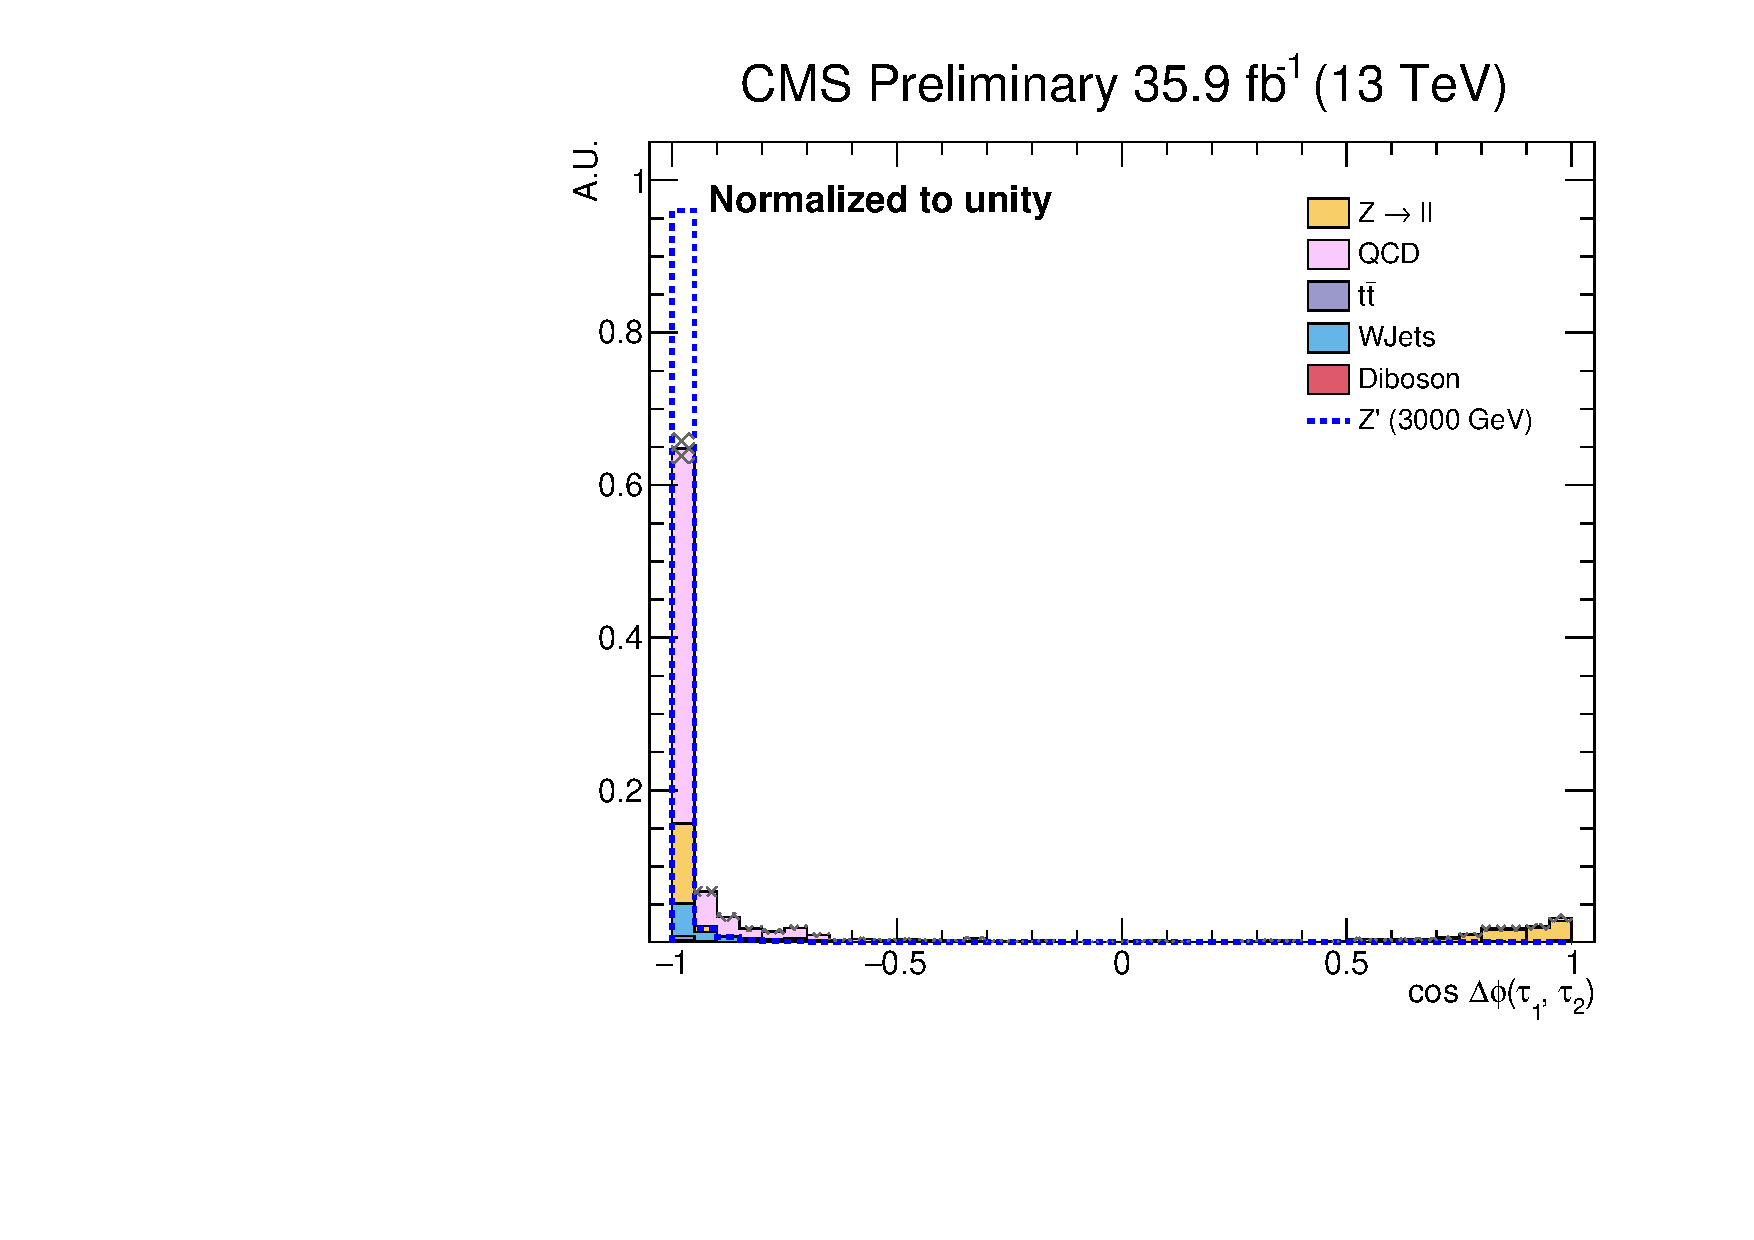
\includegraphics[clip,width=0.43\textwidth]{figuras/Chapter5/TauID_Plots/EventSelection_cosDphi.pdf}
 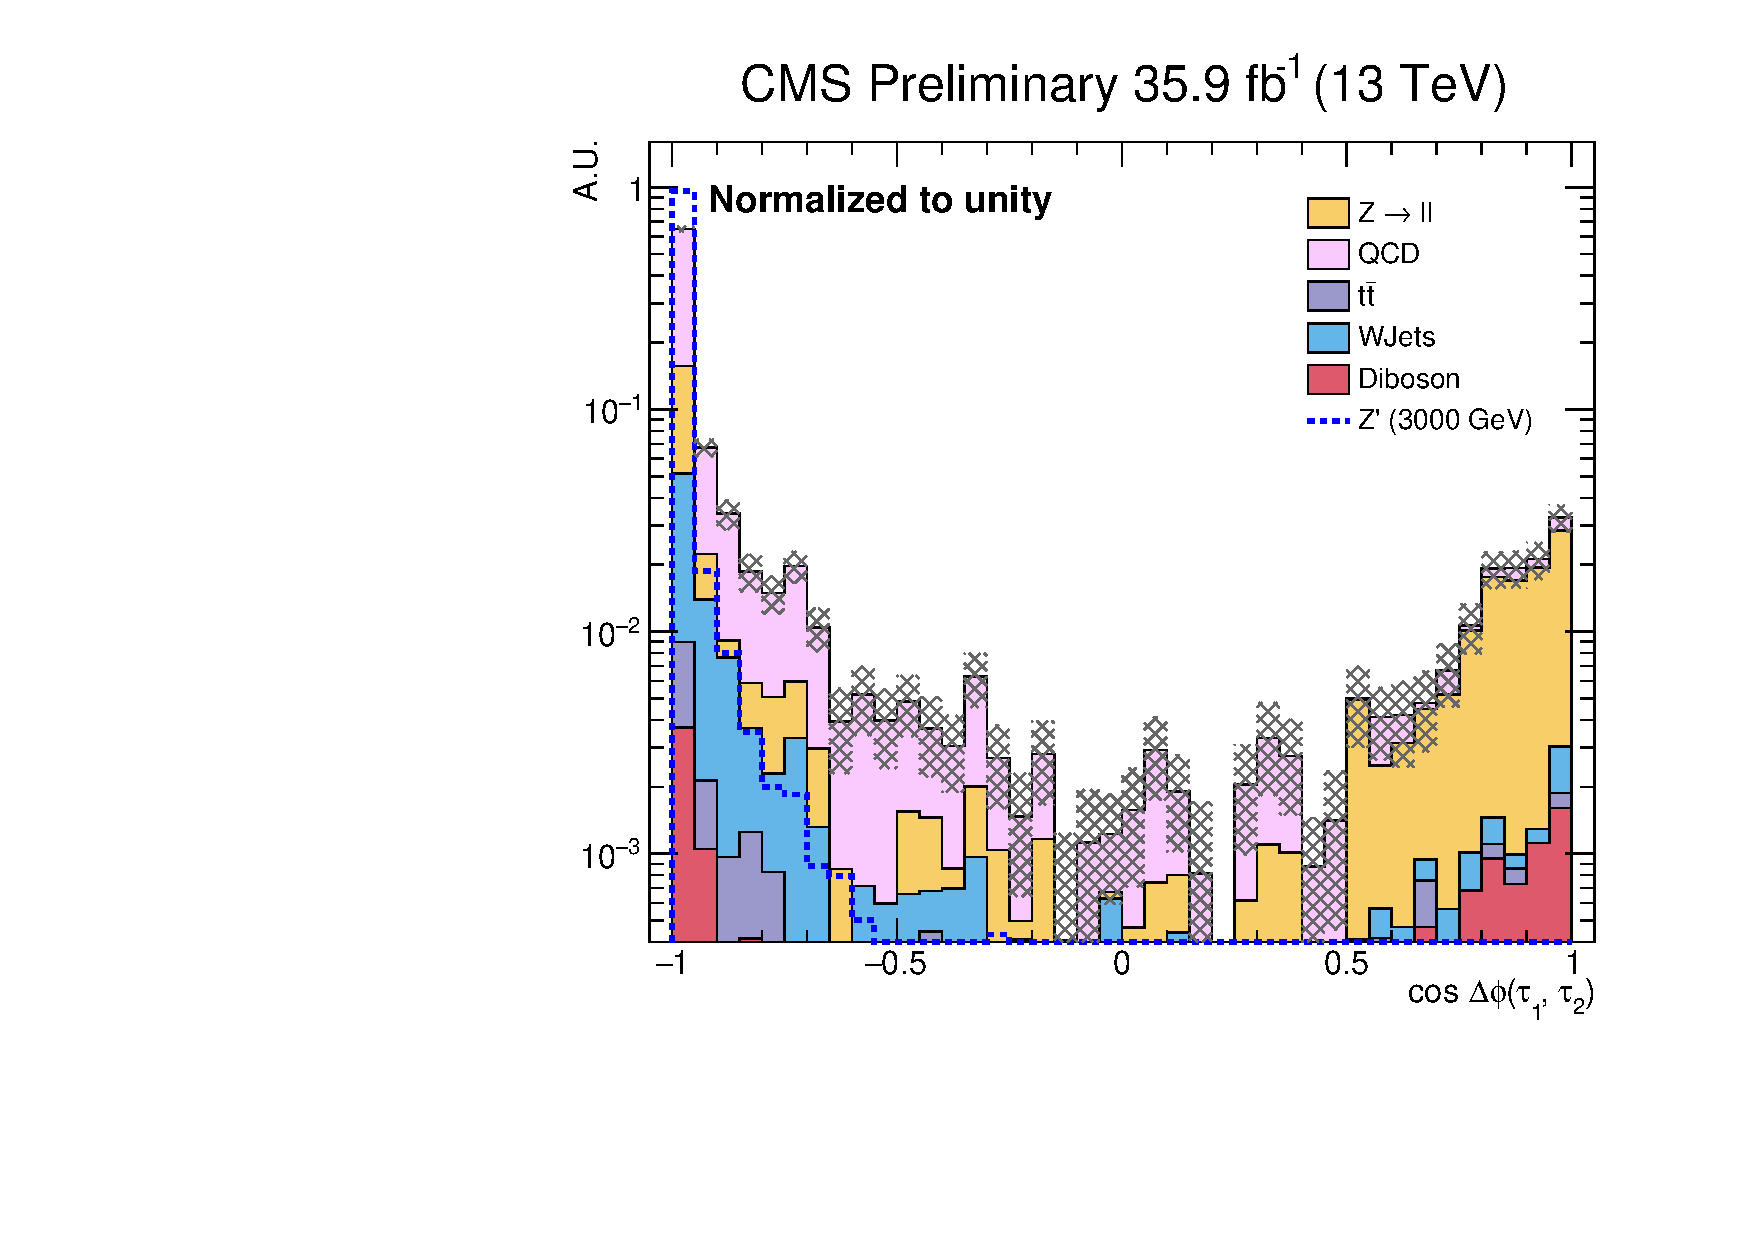
\includegraphics[clip,width=0.43\textwidth]{figuras/Chapter5/TauID_Plots/EventSelection_cosDphi_log.pdf}
 \end{center}
 \caption{$\cos\Delta \phi (\tau_{1},\tau_{2})$ distribution, normalized to unity, in linear (left) and log (right) scale, after requiring
 the tau identification, \MET, and b-jet veto criteria. QCD was estimated via data-driven method (see Section \ref{subsec:QCD}).}
 \label{cosDphi}
 \end{figure}

 \noindent The \METv~of the signal events is expected to be collinear with 
 the direction of the taus. Most of the times, the sum of the transverse momenta of the tau pair 
 will be aligned with the leading tau and, therefore, the \METv~would
 point towards the less energetic tau. As a result, for the signal events, 
 there is a strong correlation between the \METv~and the direction of the visible 
 decay products of the tau; in the case of the QCD and W+jets backgrounds, there is 
 not such correlation, since the jet faking the tau signature is produced 
 in a random direction. Consequently, the $\cos\Delta \phi (\tau_{lead},\not\!\!E_T) <$ -0.9 cut is 
 required in order to reduce the background contamination of processes such as 
 QCD and W+Jets (67$\%$ and 59$\%$, respectively), while keeping 86$\%$ of the 
 signal events. Figure \ref{cosDphiTauMET} shows the $\cos\Delta \phi (\tau_{lead},\not\!\!E_T)$
 distribution after applying the requirements mentioned above (tau identification, \MET, b-jet veto
 and $\cos\Delta \phi (\tau_{1},\tau_{2})$ cuts). In previous analyses, other cuts have 
 been applied, in order to consider the strong correlation for the signal events between the \METv~and the 
 direction of the visible decay products of the tau, such as the so-called 
 p$_{\zeta}$-cut, which was used for the previous version of this analysis
 using 2015 data \cite{CMSZprimetotautau2015}. For the 2016 data, the highest sensitivity
 is reached with the $\cos\Delta \phi (\tau_{lead},\not\!\!E_T) <$ -0.9 requirement. The 
 study of the sensitivity reached for different cuts is described in Appendix \ref{chap:EventSelection}.
    
%   that the $\cos\Delta \phi (\tau_{lead},\not\!\!E_T) <$ -0.9 cut
%  is the most sensitive one compared with 
%  
%  
%  However, there is not such correlation  since the jet production is not correlated 
%  with the tau decay products coming from the W boson.
 
 \begin{figure}[H]
 \begin{center}
 \captionsetup[subfloat]{farskip=0pt,captionskip=0.0cm,labelformat=empty}
 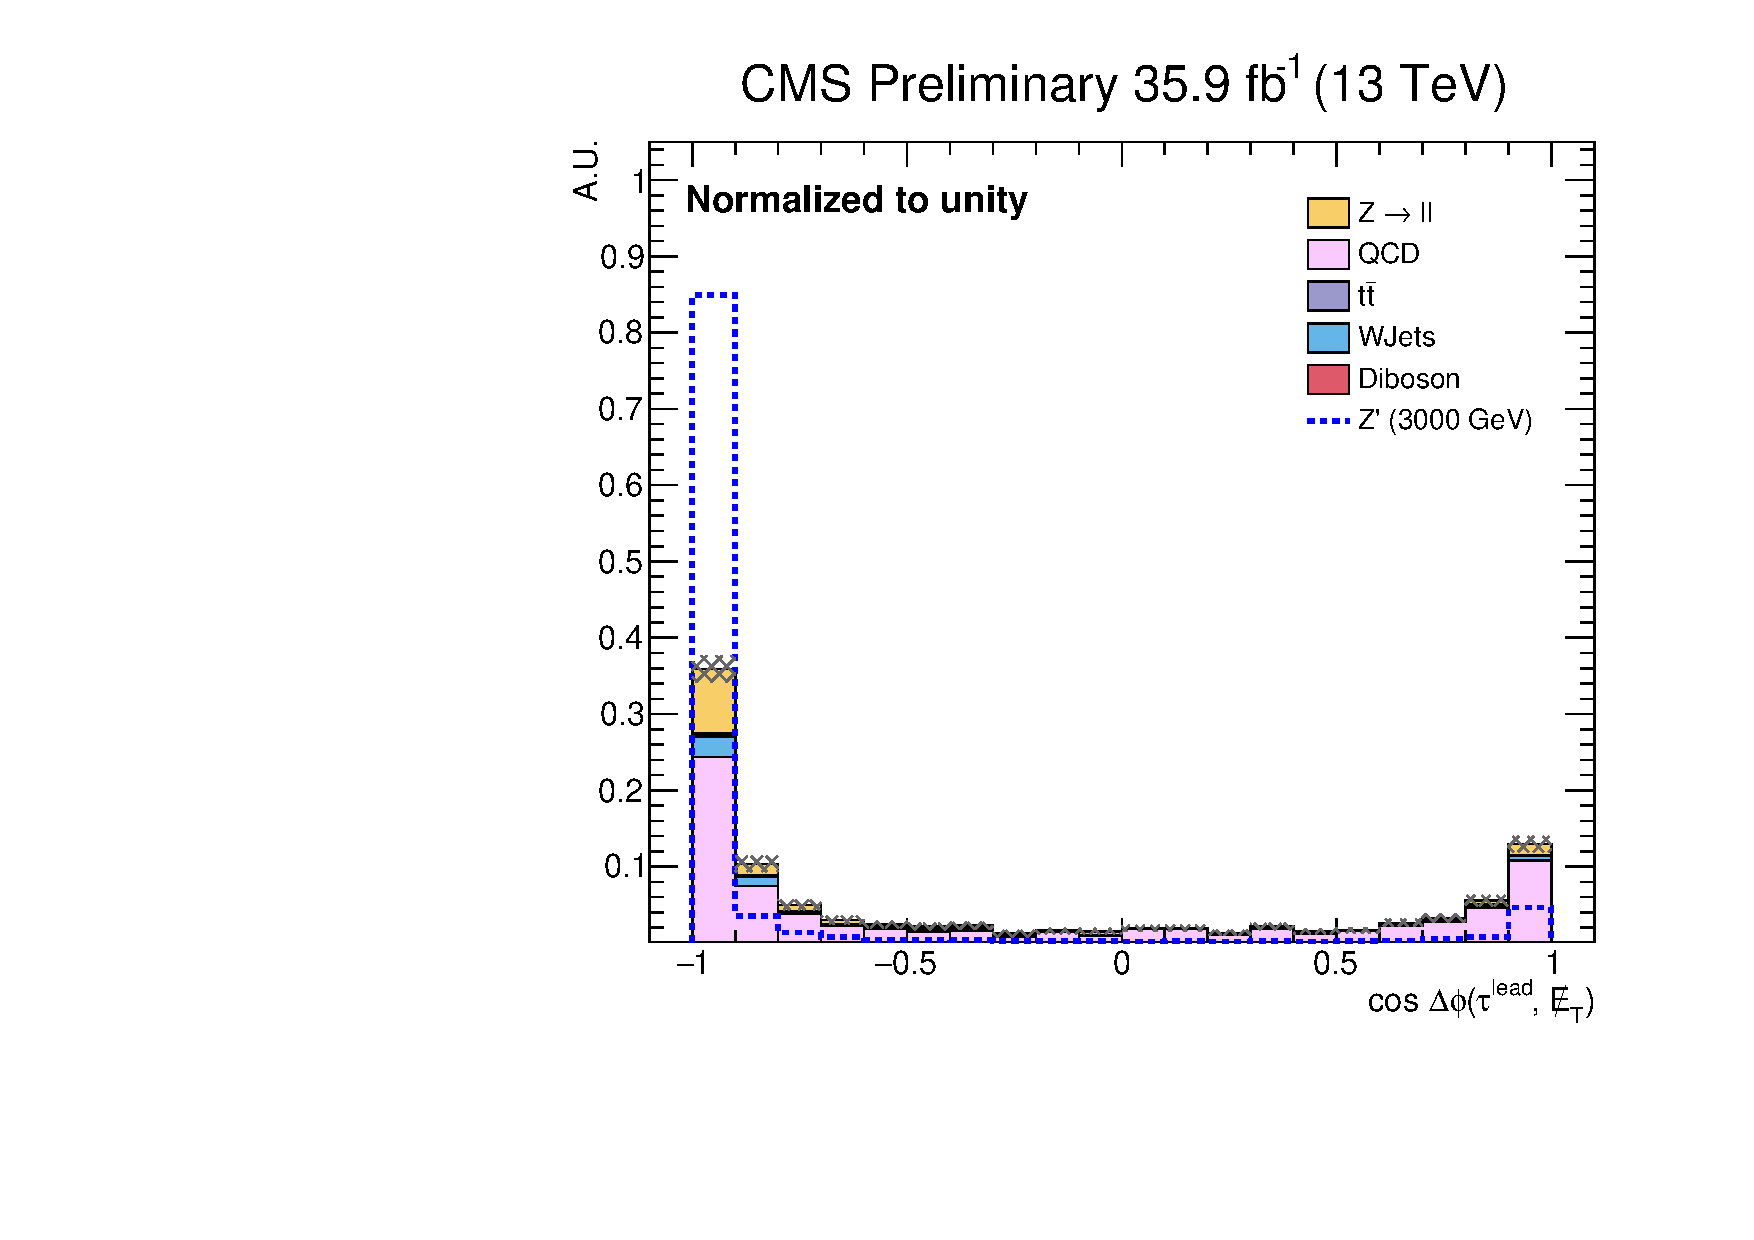
\includegraphics[clip,width=0.43\textwidth]{figuras/Chapter5/TauID_Plots/EventSelection_cosDphiTauMET.pdf}
 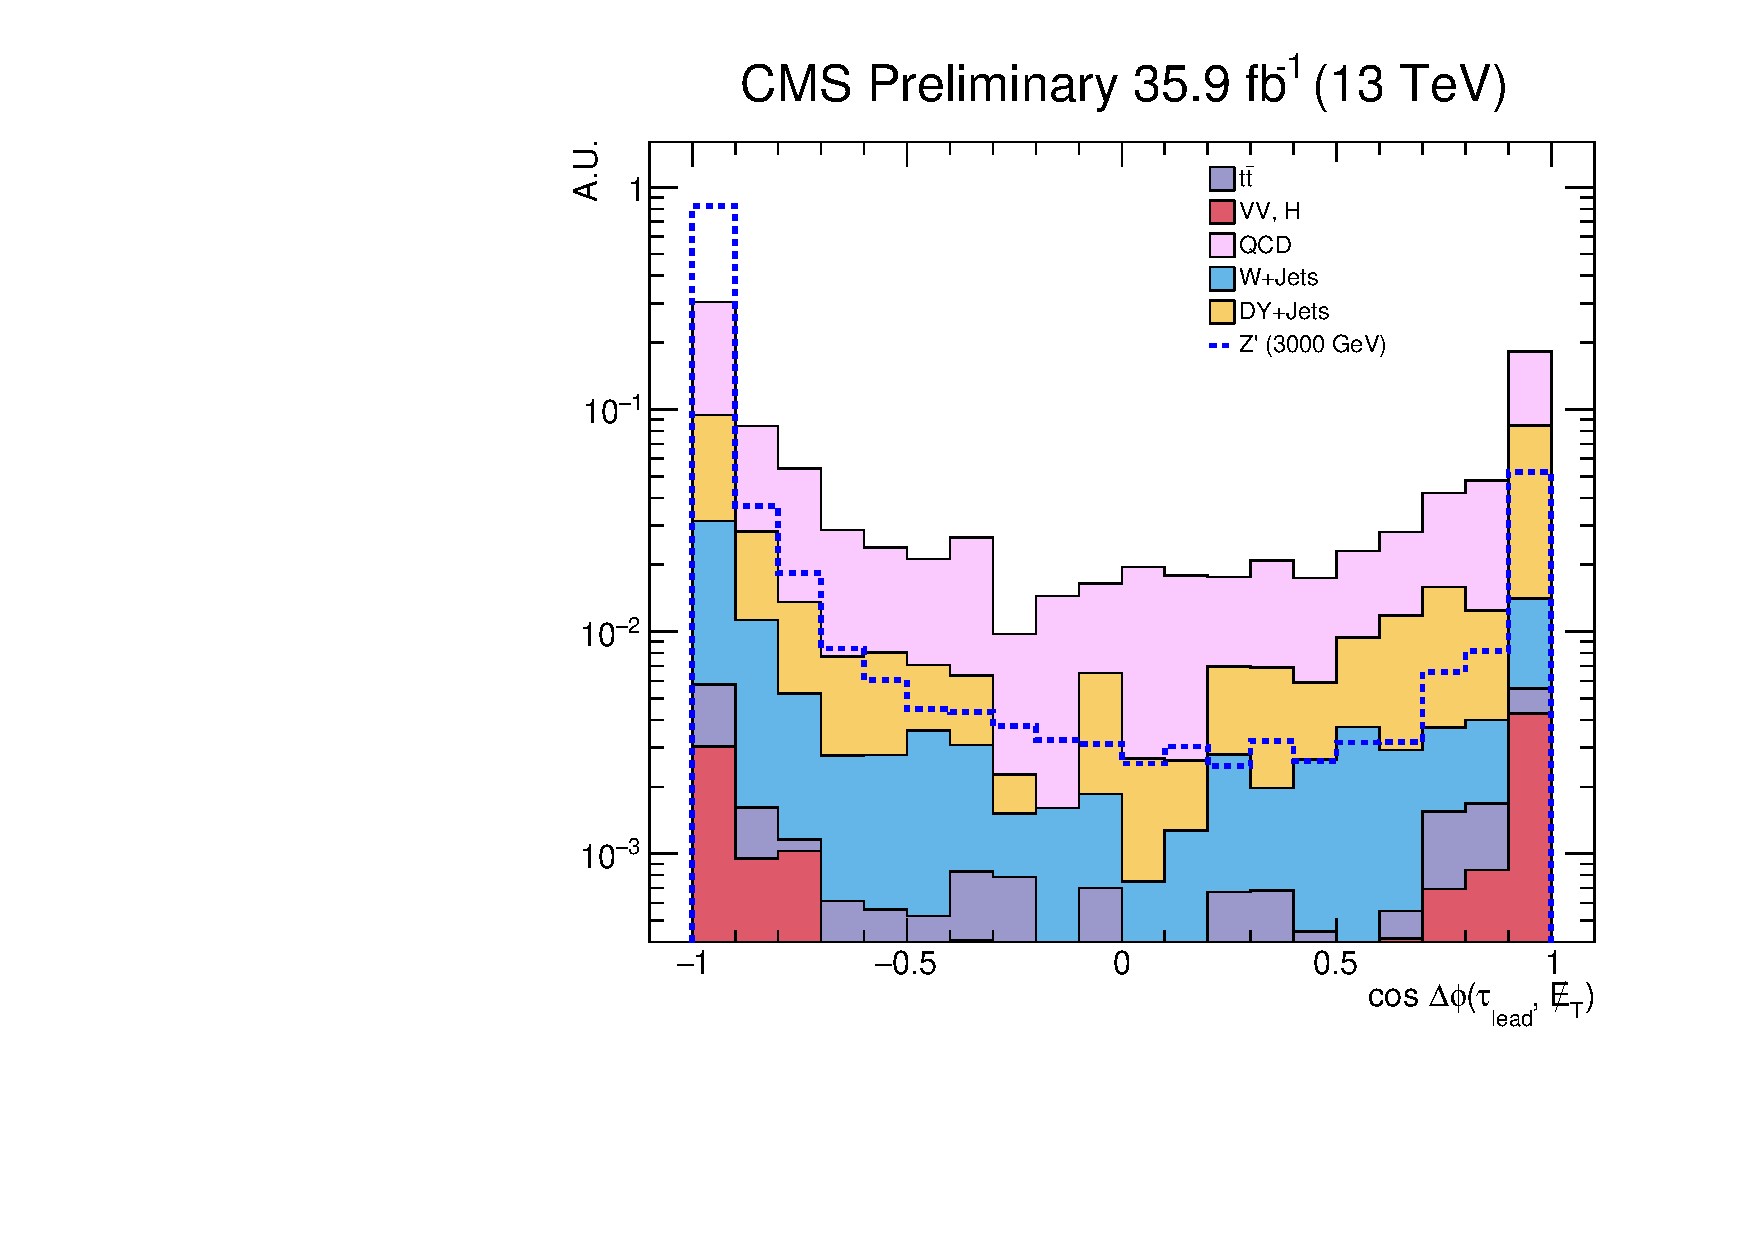
\includegraphics[clip,width=0.43\textwidth]{figuras/Chapter5/TauID_Plots/EventSelection_cosDphiTauMET_log.pdf}
 \end{center}
 \caption{$\cos\Delta \phi (\tau_{lead},\not\!\!E_T)$ distribution, normalized to unity, in linear (left) and log (right) scale, after requiring
 the tau identification, \MET, and b-jet veto criteria. QCD was estimated via data-driven method (see Section \ref{subsec:QCD}).}
 \label{cosDphiTauMET}
 \end{figure}
 
%  that could randomly give rise to two back-to-back hadronic taus.


\subsection{Summary}
\label{subsec:SignalRegion}

\noindent The tau identification criteria and the topological requirements described 
in the previous sections allow to maintain a high selection efficiency 
for signal events, providing a strong background suppression, while 
keeping a reduced influence of systematic effects. The final selection 
criteria used in this analysis, known as signal region, is presented in 
Table \ref{tab:signalRegion}.\\

\noindent The relative efficiency, as well as the cumulative efficiency
of each topological cut, for the signal and the backgrounds,
are presented in Table \ref{tab:signalRegionEff}. As can be seen, 
these topological cuts reduce the contamination of backgrounds mainly from
$t\bar{t}$, W+Jets and DiBoson processes to negligible levels.\\

\begin{table}[H]
    \centering{
 \begin{tabular}{l|l} \hline \hline 
 \pt                          &  $>$  70 \GeV \\
 $|\eta|$                     &  $<$ 2.1 \\
 Tau Decay                     & \textit{1or3-prongs} \\
                              & \textit{newDMF} \\
 Isolation Disc.              & \textit{byTightIsolationMVArun2v1DBnewDMwLT} \\
 Anti-electron Disc.          & \textit{againstElectronMVALooseMVA6} \\
 Anti-muon Disc.              & \textit{againstMuonTight3} \\ \hline \hline 
 \MET                         & $>$ 30 \GeV \\
 $\#$ b-jets (CSVv2 Loose WP) & $= 0$ \\
 $Ch_{\tau_{1}} \times Ch_{\tau_{2}} $ & $<$ 0 \\
 \DRt                         & $>$ 0.3  \\
 $\cos\Delta \phi (\tau_{1},\tau_{2})$ & $<$ -0.95  \\
 $\cos\Delta \phi (\tau_{lead},\not\!\!E_T)$ & $<$ -0.90 \\ \hline \hline 
  \end{tabular}
  \caption{Signal Region} \label{tab:signalRegion}
  }
  
\end{table}

\begin{table}[H]
\resizebox{\textwidth}{!}{
%     \centering{
 \begin{tabular}{|l|c|c|c|c|c|c|c|c|c|c|c|c|} \hline \hline 
Cut             &      \multicolumn{2}{|c|}{QCD}       &        \multicolumn{2}{|c|}{DY}      &    \multicolumn{2}{|c|}{W+Jets}     &  \multicolumn{2}{|c|}{$t\bar{t}$}    &     \multicolumn{2}{|c|}{DiBoson}   &  \multicolumn{2}{|c|}{\Zprime~[3 \TeV]}   \\ \hline \hline
%                 &  $\epsilon$ [$\%$] & Cumulative $\epsilon$ [$\%$] &  $\epsilon$ [$\%$] & Cumulative $\epsilon$ [$\%$] & $\epsilon$ [$\%$] & Cumulative $\epsilon$ [$\%$] &  $\epsilon$ [$\%$] & Cumulative $\epsilon$ [$\%$] & $\epsilon$ [$\%$] & Cumulative $\epsilon$ [$\%$] &  $\epsilon$ [$\%$]  & Cumulative $\epsilon$ [$\%$]  \\ \hline
                &  $\epsilon$ [$\%$] & Cum $\epsilon$ [$\%$] &  $\epsilon$ [$\%$] & Cum $\epsilon$ [$\%$] & $\epsilon$ [$\%$] & Cum $\epsilon$ [$\%$] &  $\epsilon$ [$\%$] & Cum $\epsilon$ [$\%$] & $\epsilon$ [$\%$] & Cum $\epsilon$ [$\%$] &  $\epsilon$ [$\%$]  & Cum $\epsilon$ [$\%$]  \\ \hline
%  NRecoVertex												
Trigger         & 56.0       &  56.0285	                &   100.00  &	100.00            &   100.00  &	100.00        &   100.00   &      100.00       &  100.00   &	100.00       & 100.0   &   100.0   \\
TauID 1         &  0.9       &	 0.5029                 &     0.03  &	0.03046           &	0.03  &	0.02526       &     0.40   &	    0.40367    &    0.30   &	  0.2971     &	43.0   &    43.0   \\
TauID 2         &  0.5       &   0.0023                 &     0.73  &	0.00022           &	0.07  &	0.000017      &	    0.18   &	    0.00071    &    0.69   &      0.0021     &	14.5   &     6.3   \\
\MET~cut        & 47.3       &	 0.0011                 &    61.79  &	0.00014           &    72.79  &	0.000012      &    83.66   &	    0.00059    &   75.76   &	  0.0016     &	93.8   &     5.9   \\
b-jet veto      & 88.0       &   0.0009                 &    83.78  &   0.00011	          &    90.57  &	0.000011      &    23.27   &        0.00014    &   78.07   &      0.0012     &  90.0   &     5.3   \\
$\cos\Delta \phi(\tau_{1},\tau_{2})$    & 24.7 & 0.0002 &    38.92  &	0.00004	          &    40.41  &	0.000004      &	   34.88   &	    0.00005    &   23.20   &      0.0003     &	81.5   &     4.3   \\
$\cos\Delta \phi(\tau_{lead},\not\!\!E_T)$ & 33.1 & 0.0001 &    51.73  &	0.00002           &    40.56  &	0.000002      &	   34.38   &	    0.00002    &   41.11   & 	  0.0001     &	86.4   &     3.7   \\ \hline \hline
 
 \end{tabular}
%
%   }
  }
     \caption{Efficiency ($\epsilon$) and cumulative efficiency (Cum $\epsilon$) for each selection of the signal region.}
  \label{tab:signalRegionEff}
\end{table}

\subsection{Validation Plots for Signal Selections}
\label{subsec:ValidationSignalSelections}

The performance of the signal selections is validated using \textit{(N-1) distributions}.
An (N-1) distribution corresponds to the case when all the signal region cuts
are applied with exception of one of them; this allows to enhance 
the background contribution relevant to the dropped selection in order
to probe the level of accuracy between the MC samples and the data. For instance, the 
validation of the \MET~selection is performed checking the 
data and MC samples agreement for the \MET~distribution, after applying 
all the signal selection criteria with exception of this cut. Figure \ref{nminusone_MC} shows 
some (N-1) plots for the signal region using the MC samples described in 
Table \ref{tab:mc_samples}. As can be seen in the figure, QCD MC samples 
have limited statistics with considerable uncertainties, which 
motivates a data-driven estimation of this background. Figure \ref{nminusone} presents
the (N-1) plots using a data-driven method for the QCD 
estimation (see section \ref{subsec:QCD}). As expected, the (N-1) 
distributions are dominated by the QCD background; the good agreement 
between the background and data validates the QCD data-driven estimation, as well
as the MC samples used.


\begin{figure}[H]
  %
\begin{center}
 \captionsetup[subfloat]{farskip=0pt,captionskip=0.0cm,labelformat=empty}
\resizebox{\textwidth}{8.8cm}{ 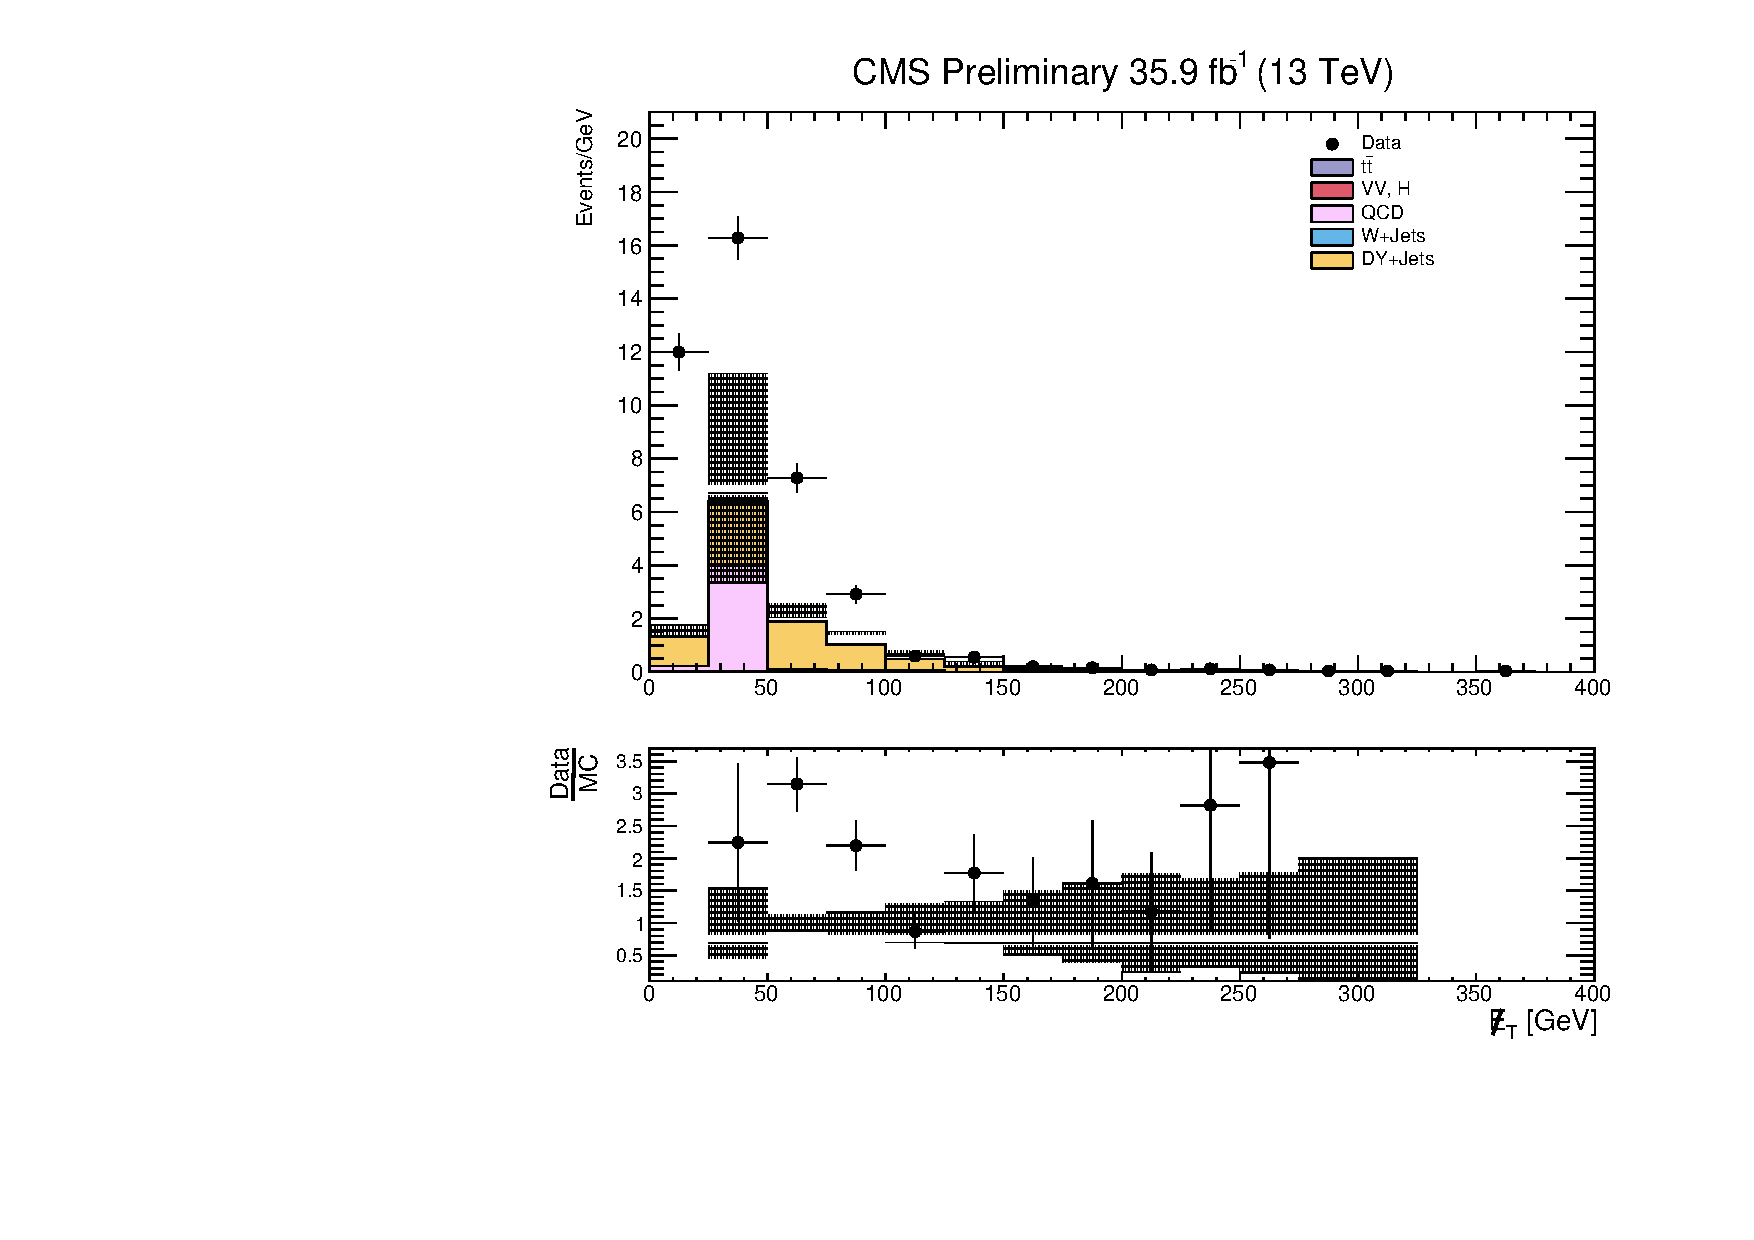
\includegraphics[clip,width=0.46\textwidth]{figuras/Chapter5/NminusOne_QCD_MC/noMET_QCD_MC.pdf}
 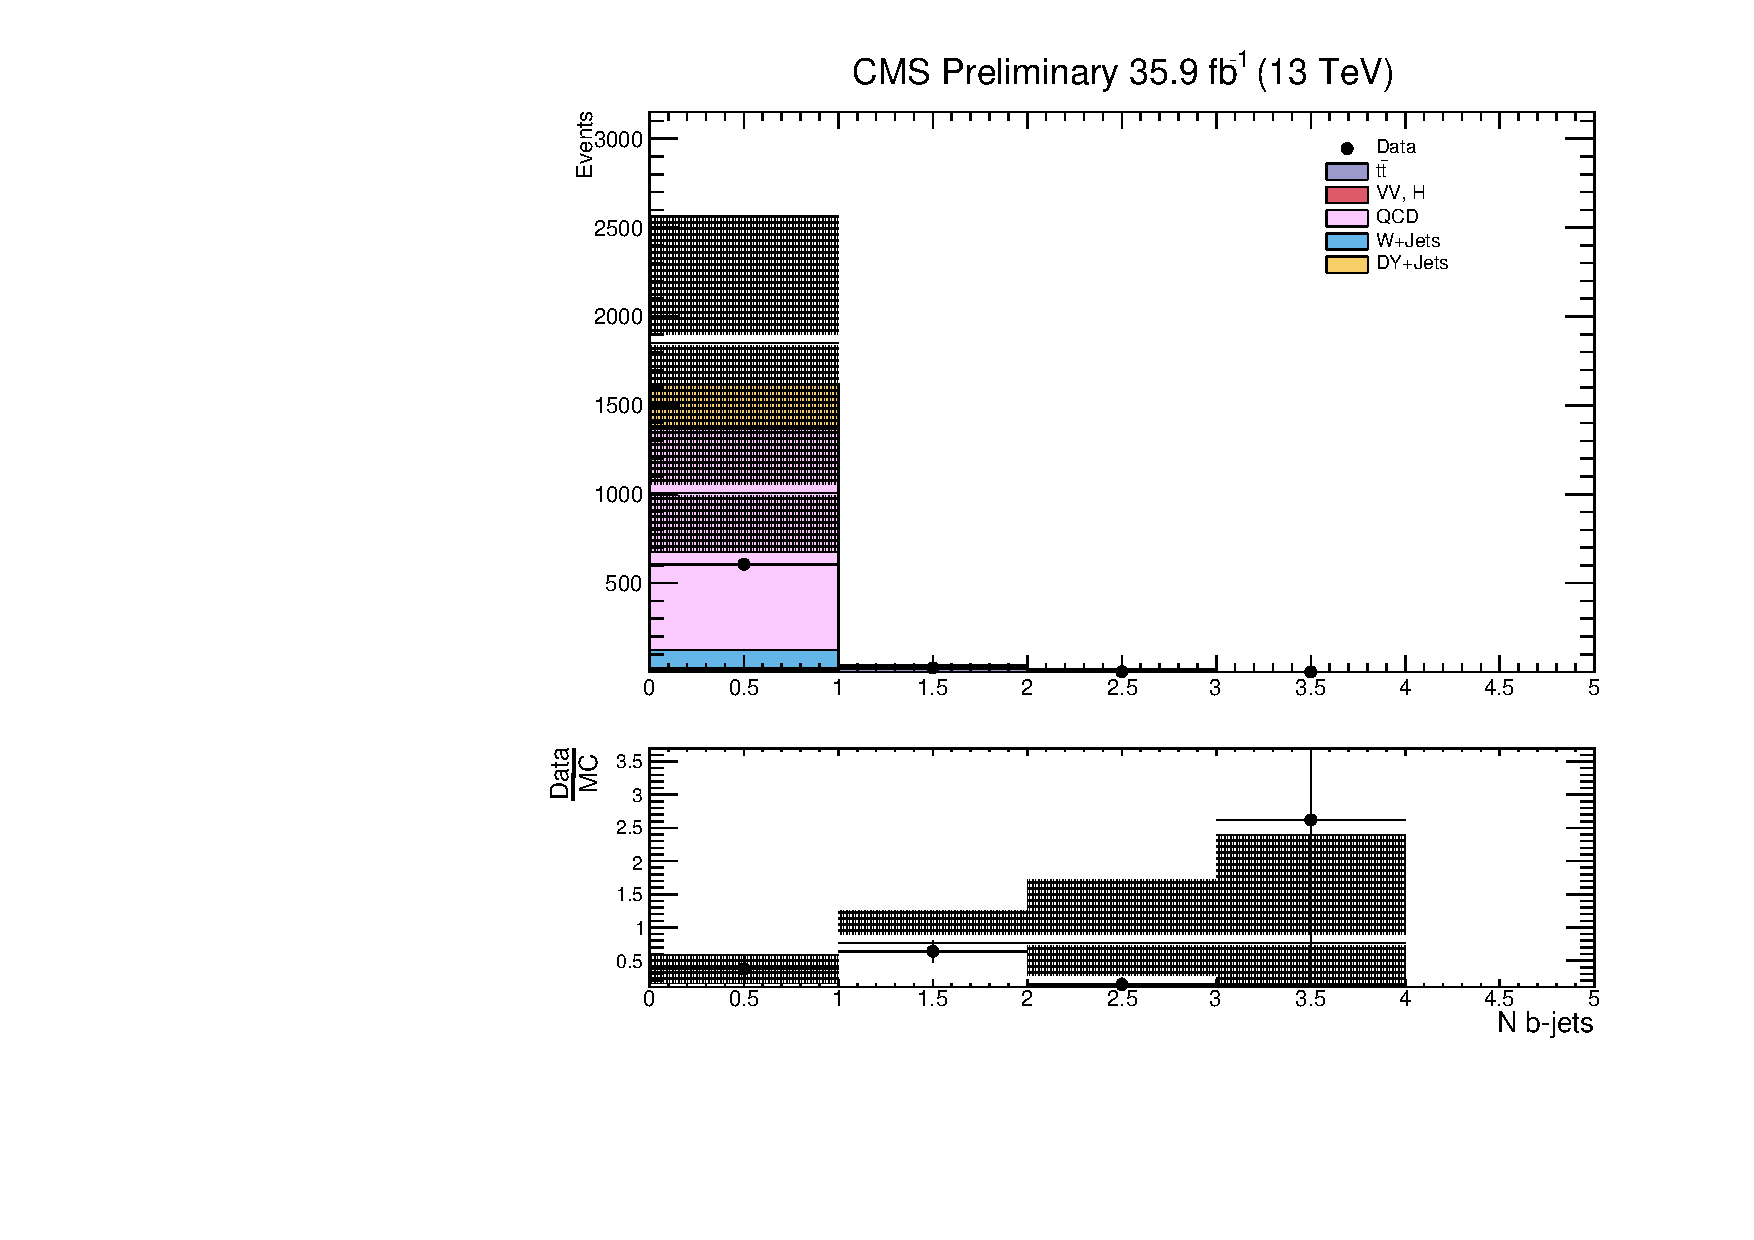
\includegraphics[clip,width=0.46\textwidth]{figuras/Chapter5/NminusOne_QCD_MC/noBjet_QCD_MC.pdf}}
 \resizebox{\textwidth}{8.8cm}{
 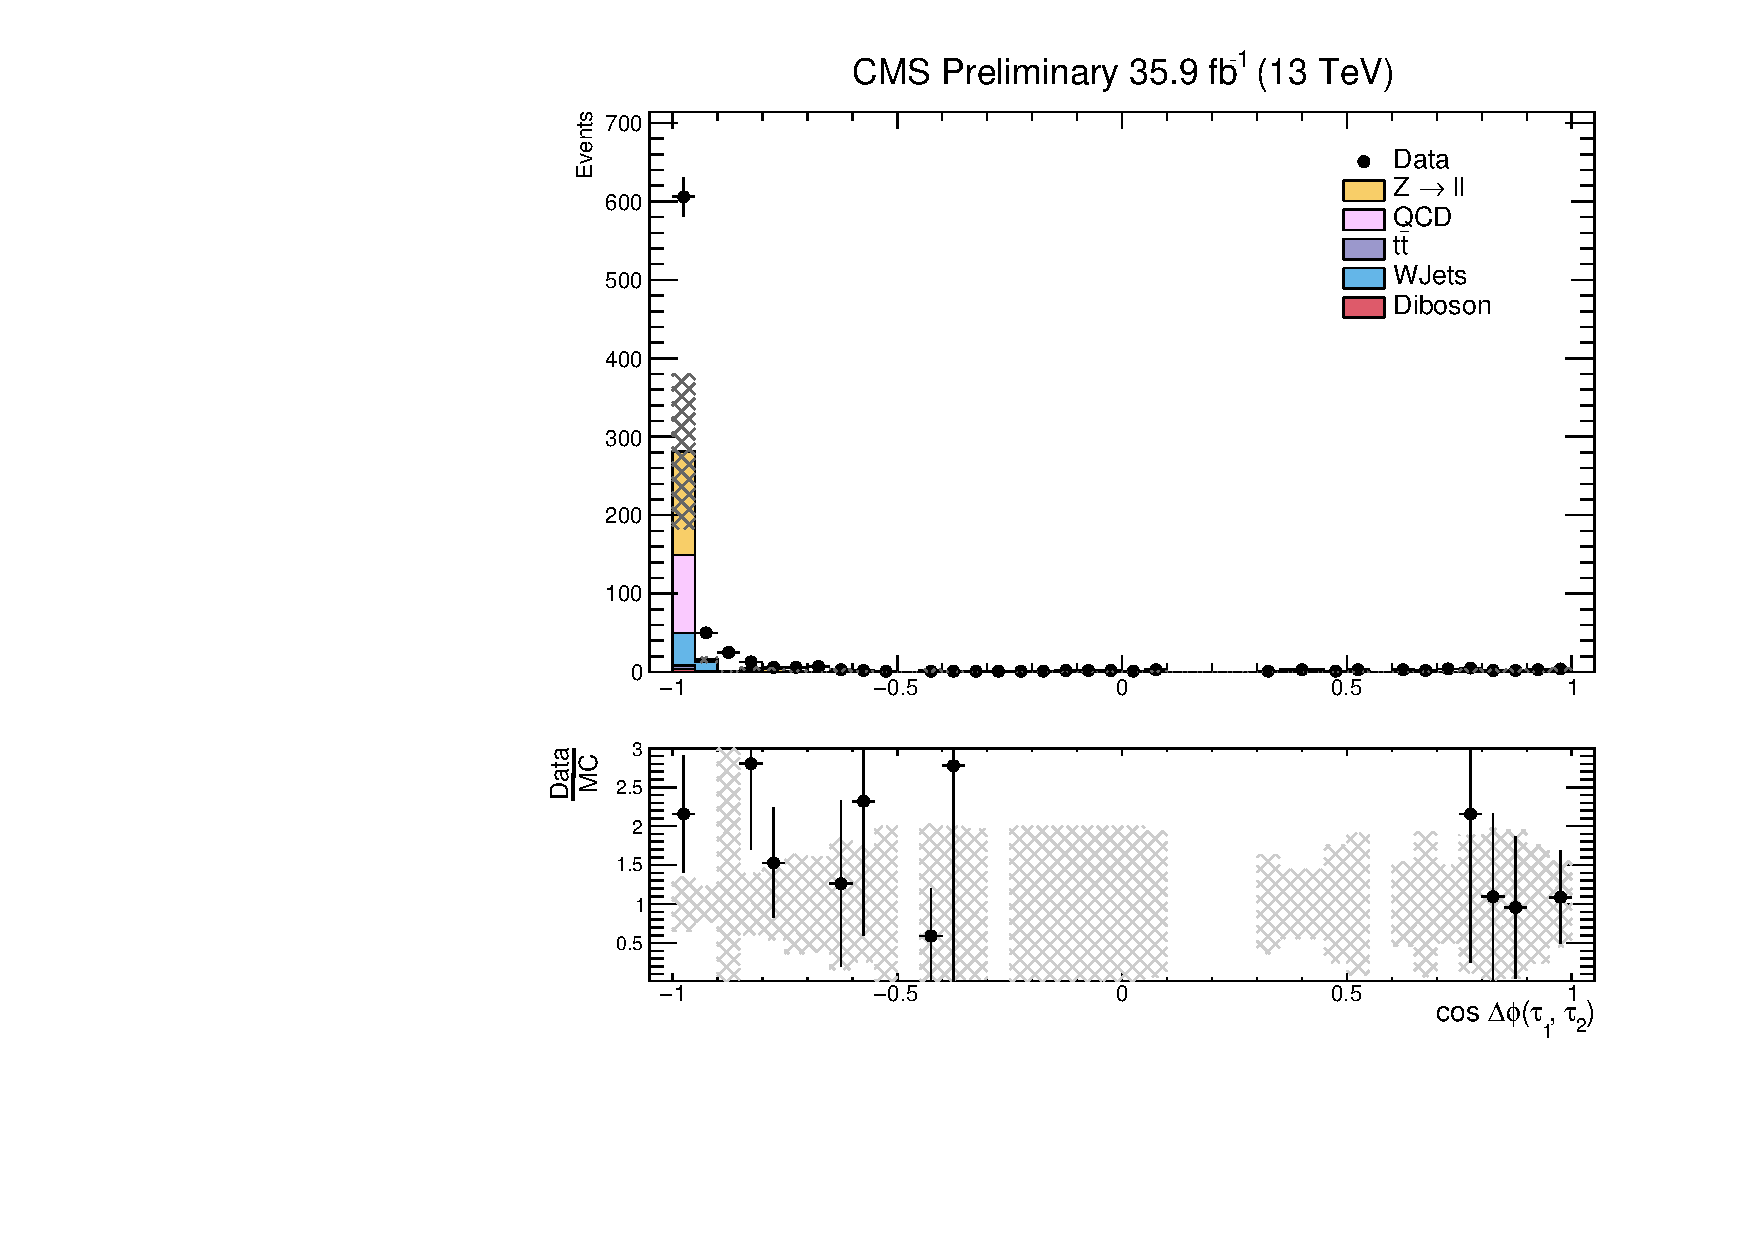
\includegraphics[clip,width=0.46\textwidth]{figuras/Chapter5/NminusOne_QCD_MC/noCosDphi_QCD_MC.pdf}
 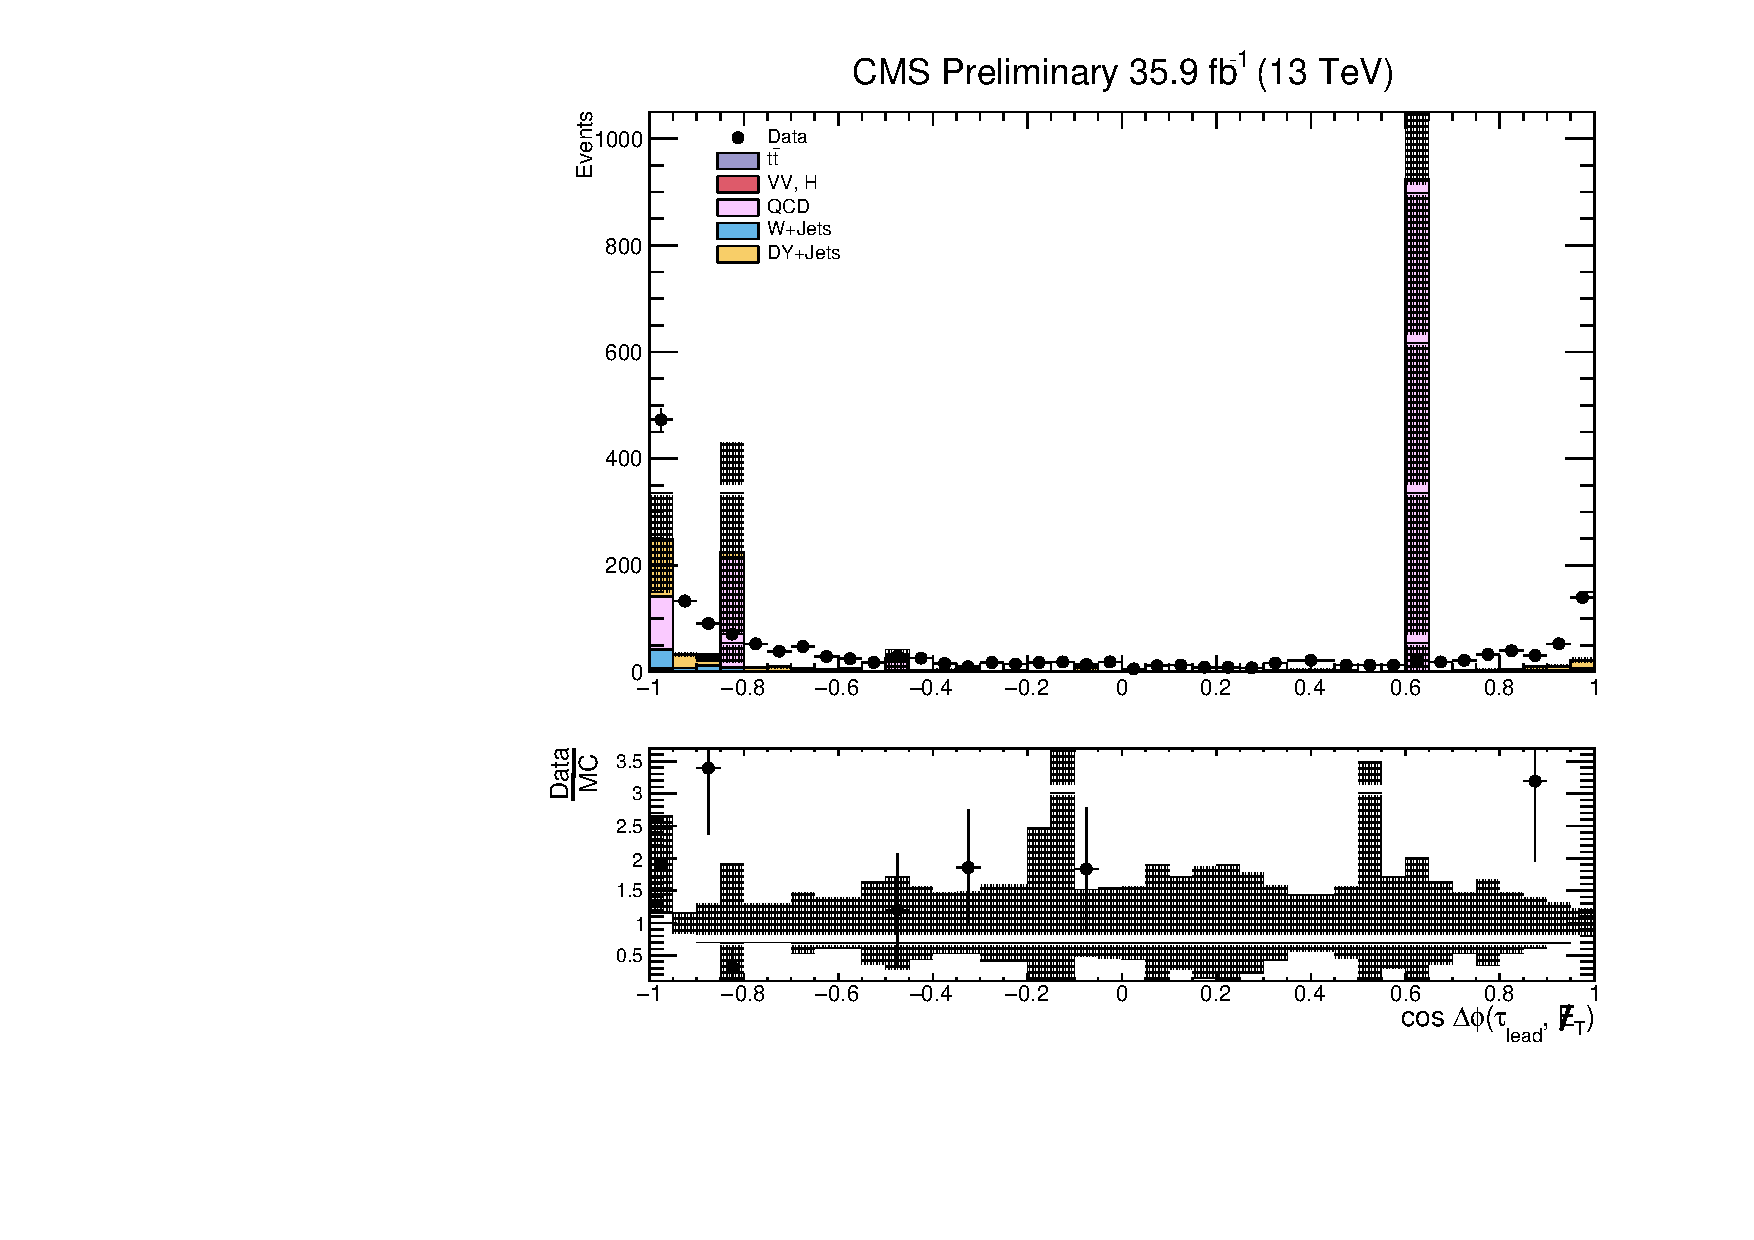
\includegraphics[clip,width=0.46\textwidth]{figuras/Chapter5/NminusOne_QCD_MC/noCosDphiTauMET_QCD_MC.pdf}}
 \end{center}
 \caption{Distribution of variables after all requirements for the signal region, with the exception of the
one plotted: \MET~(top left), number of b-jets (top right), $\cos\Delta \phi (\tau_{1},\tau_{2})$ (bottom left), 
$\cos\Delta \phi (\tau_{lead}, \not\!\!E_T)$ (bottom right). The QCD estimation was performed using the MC samples listed in Table \ref{tab:mc_samples}.}
\label{nminusone_MC} 
 \end{figure}
 
 \begin{figure}[H]
 \begin{center}
 \captionsetup[subfloat]{farskip=0pt,captionskip=0.0cm,labelformat=empty}
 \resizebox{\textwidth}{8.8cm}{
 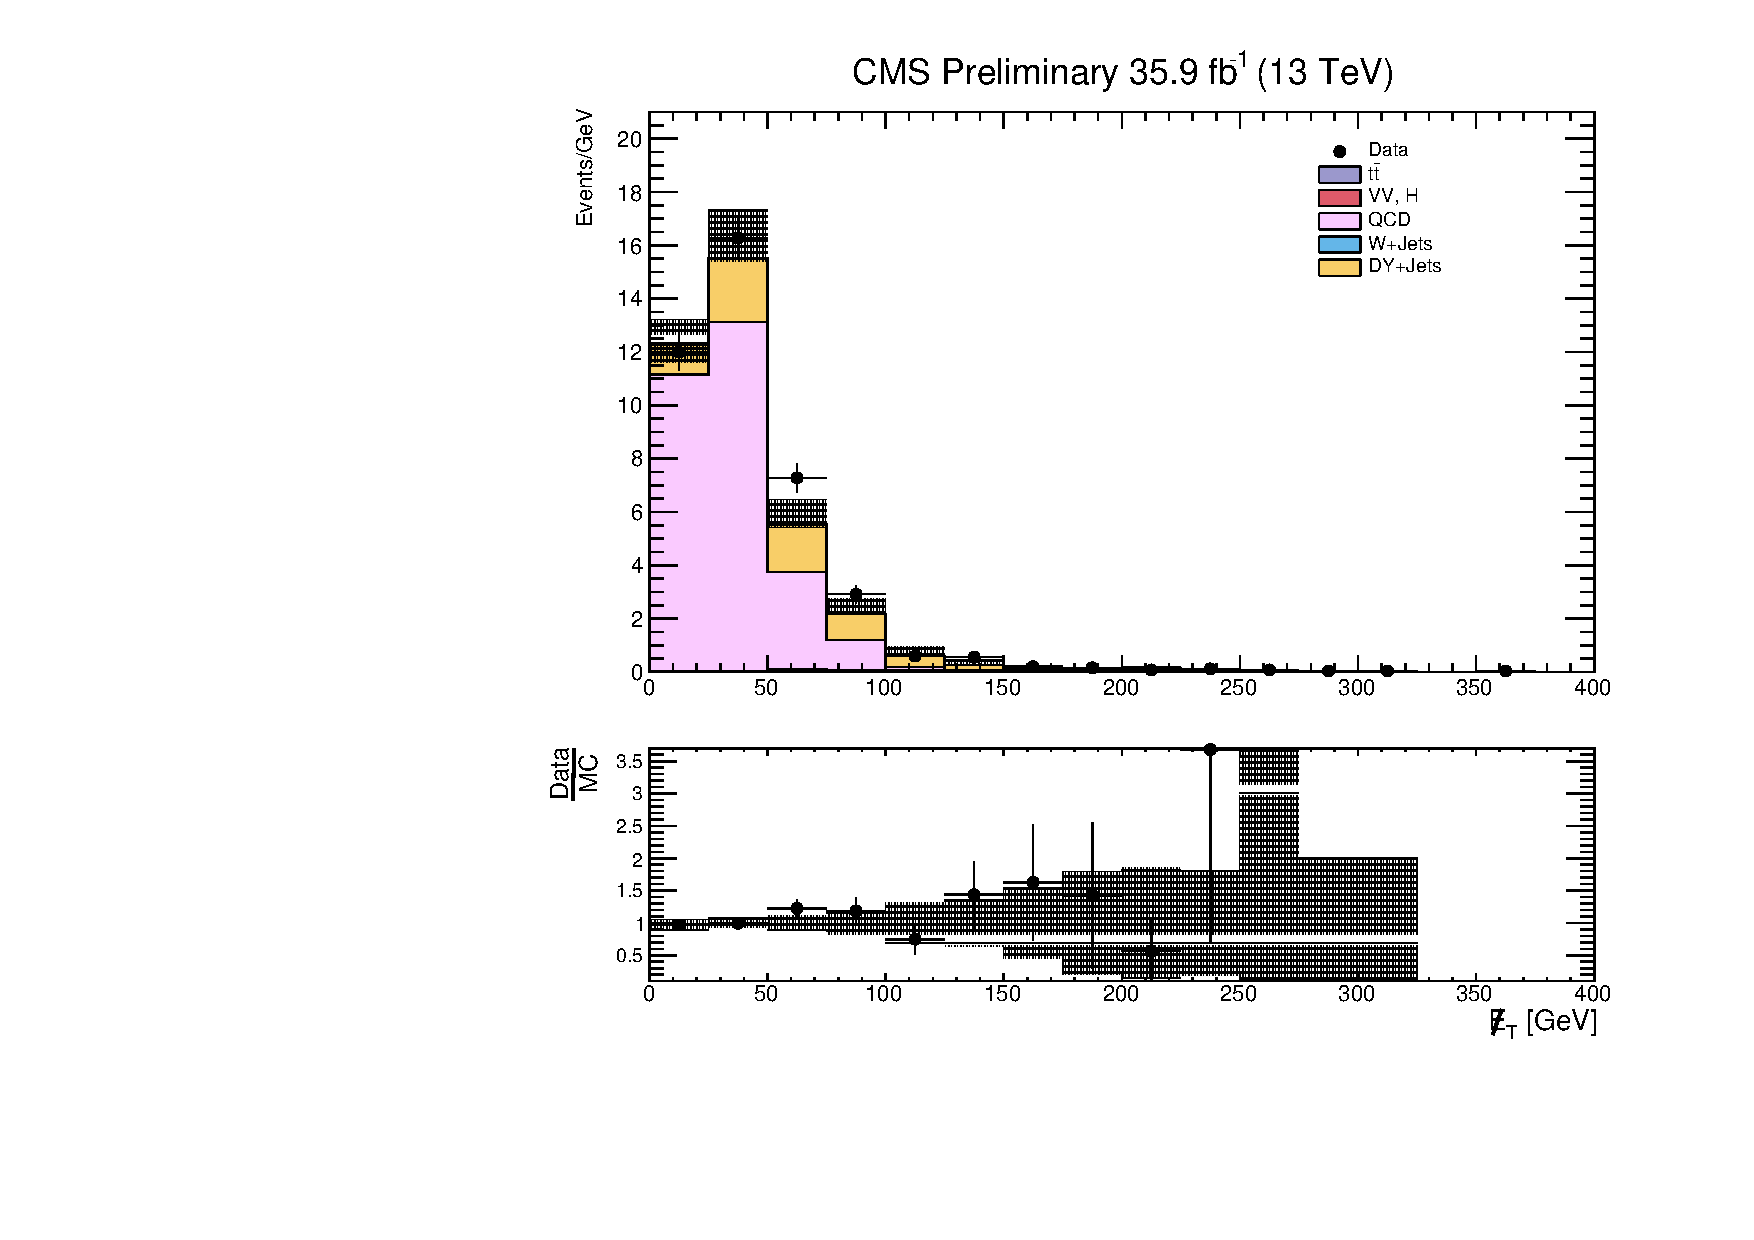
\includegraphics[clip,width=0.46\textwidth]{figuras/Chapter5/NminusOne/noMET.pdf}
 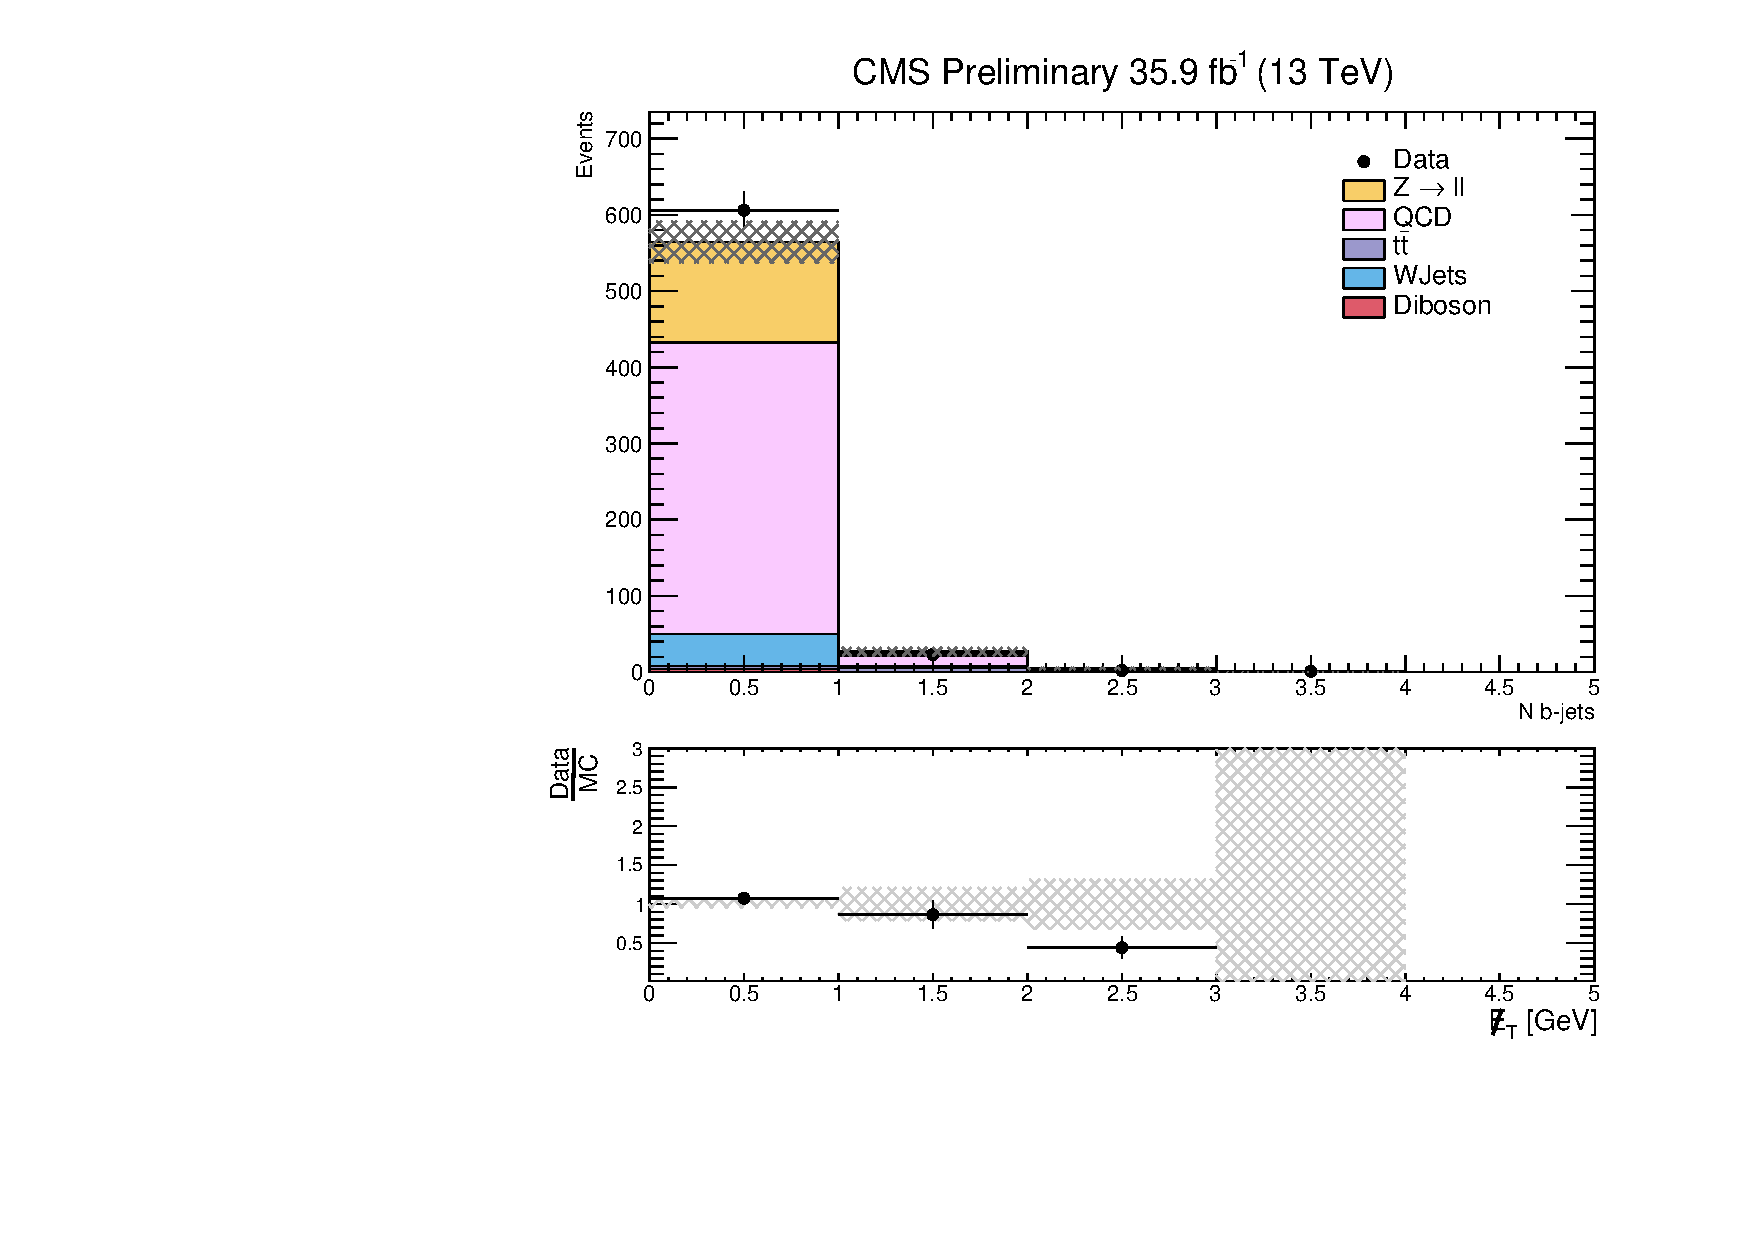
\includegraphics[clip,width=0.46\textwidth]{figuras/Chapter5/NminusOne/noBjet.pdf}}
 \resizebox{\textwidth}{8.8cm}{
 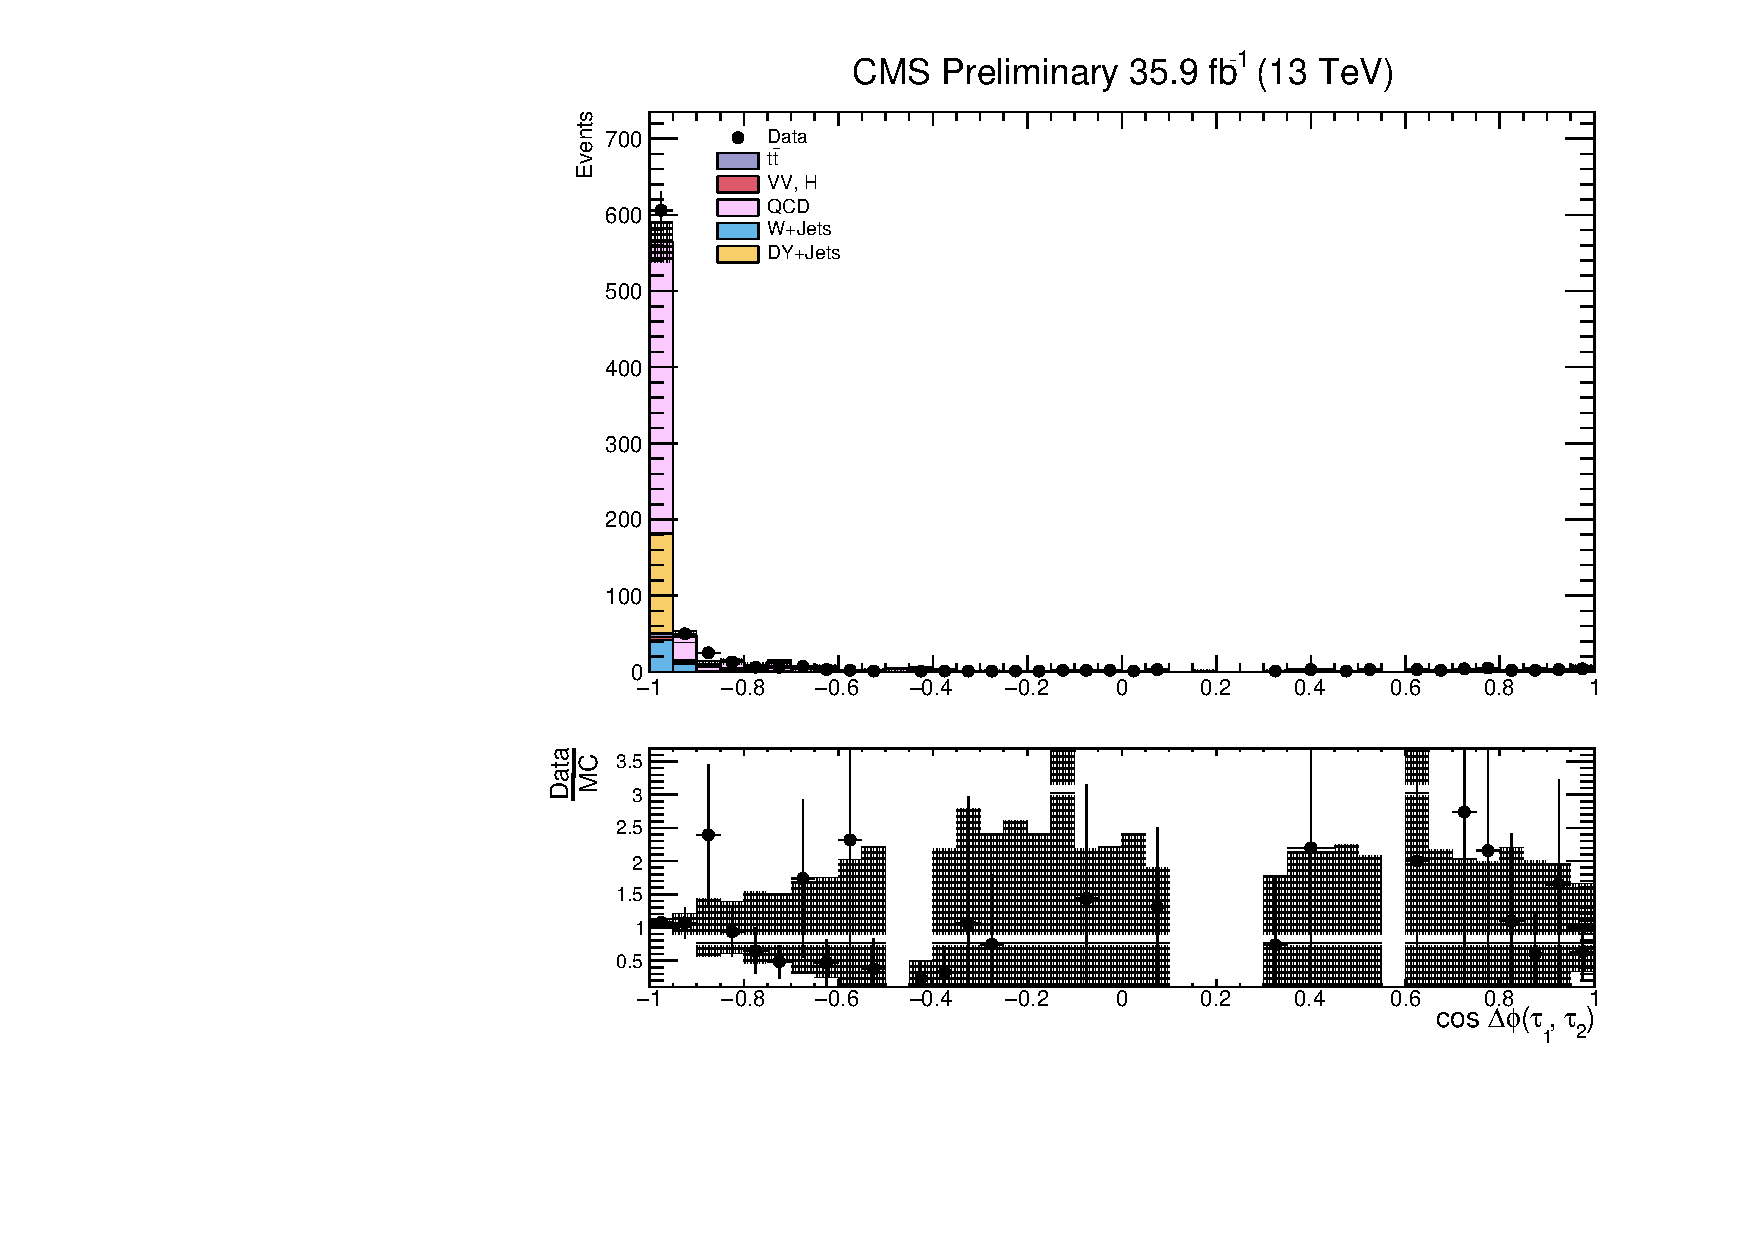
\includegraphics[clip,width=0.46\textwidth]{figuras/Chapter5/NminusOne/noCosDphi.pdf}
 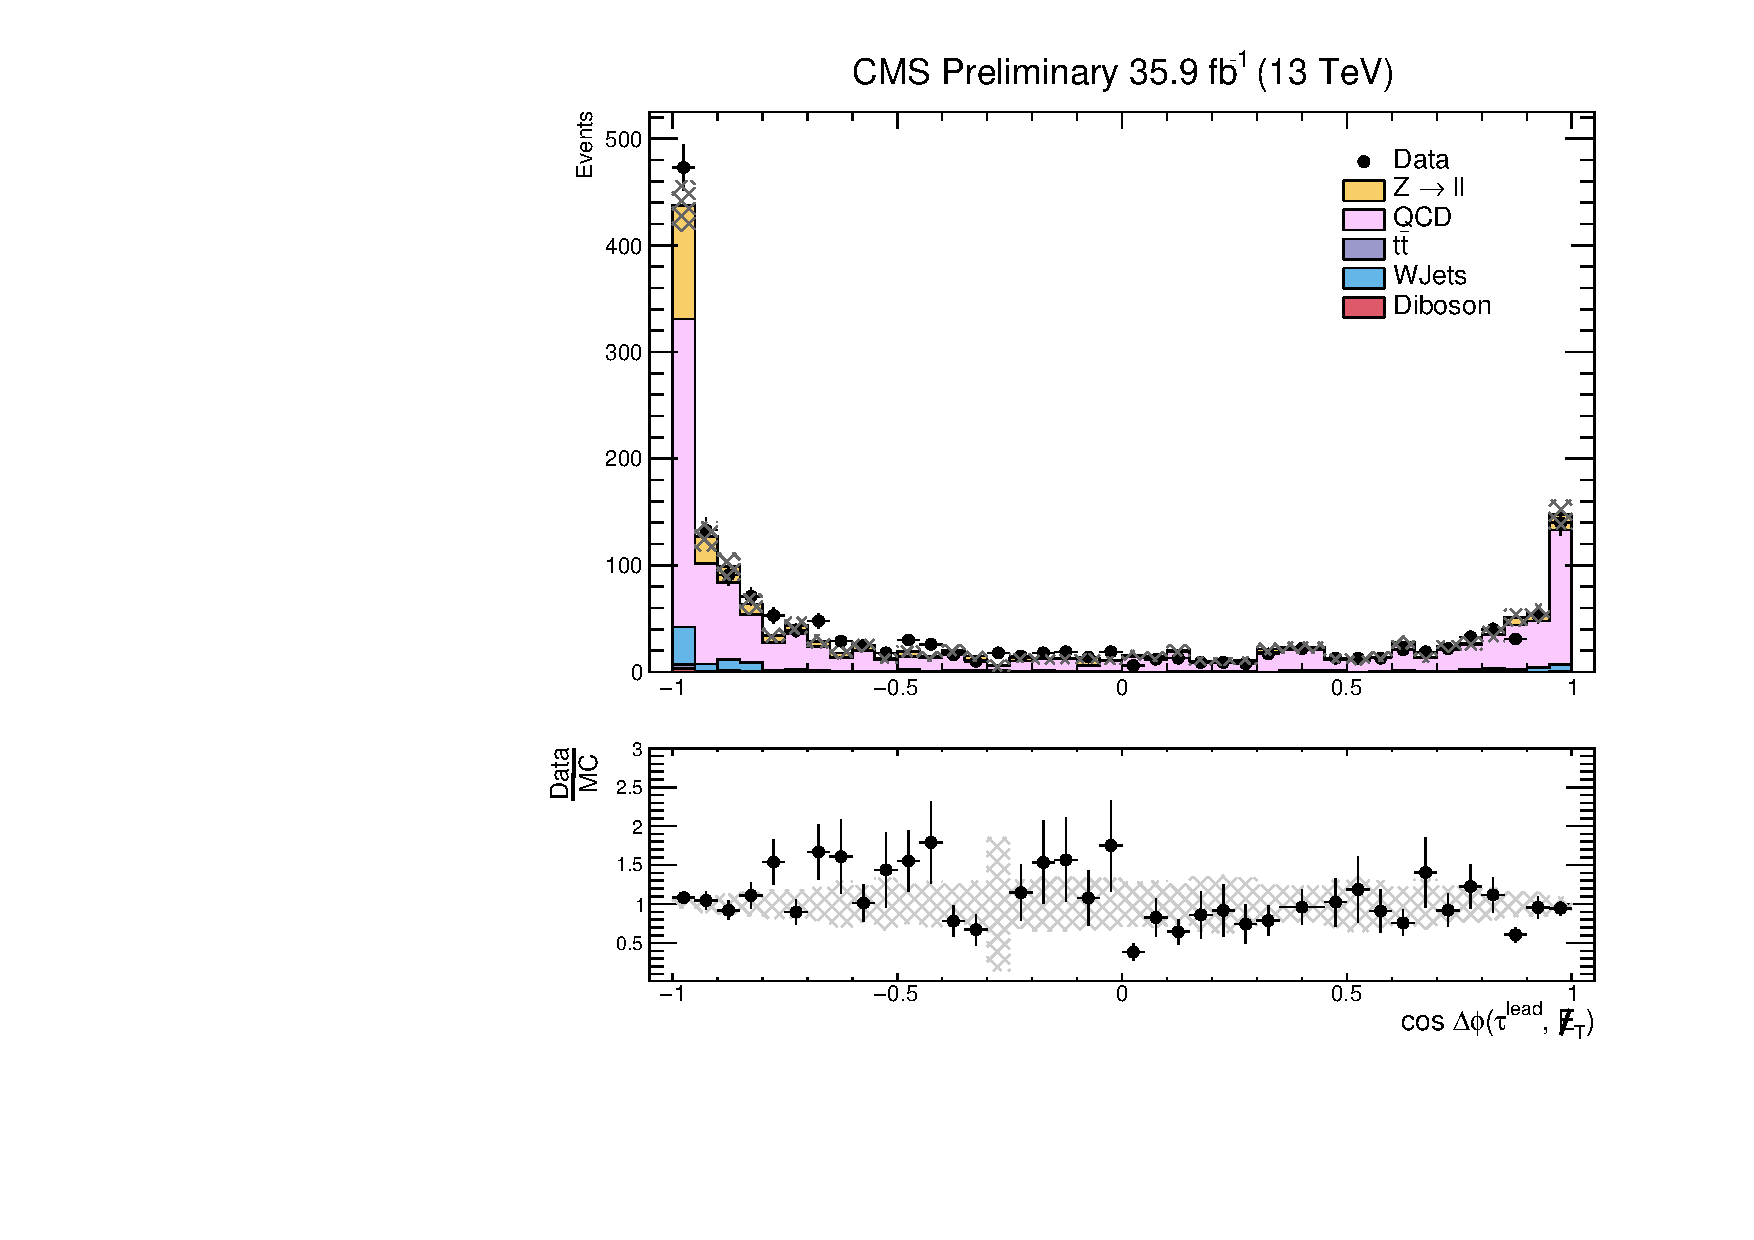
\includegraphics[clip,width=0.46\textwidth]{figuras/Chapter5/NminusOne/noCosDphiTauMET.pdf}
 }
 \end{center}
 \caption{Distribution of variables after all requirements for the signal region, with the exception of the
one plotted: \MET~(top left), number of b-jets (top right), $\cos\Delta \phi (\tau_{1},\tau_{2})$ (bottom left), 
$\cos\Delta \phi (\tau_{lead}, \not\!\!E_T)$ (bottom right). The QCD background has been estimated with 
the data-driven method described in section \ref{subsec:QCD}.}
\label{nminusone} 
 \end{figure}

%  \begin{figure}[H]
%  \begin{center}
%  \captionsetup[subfloat]{farskip=0pt,captionskip=0.0cm,labelformat=empty}
%  \resizebox{\textwidth}{8.8cm}{
%  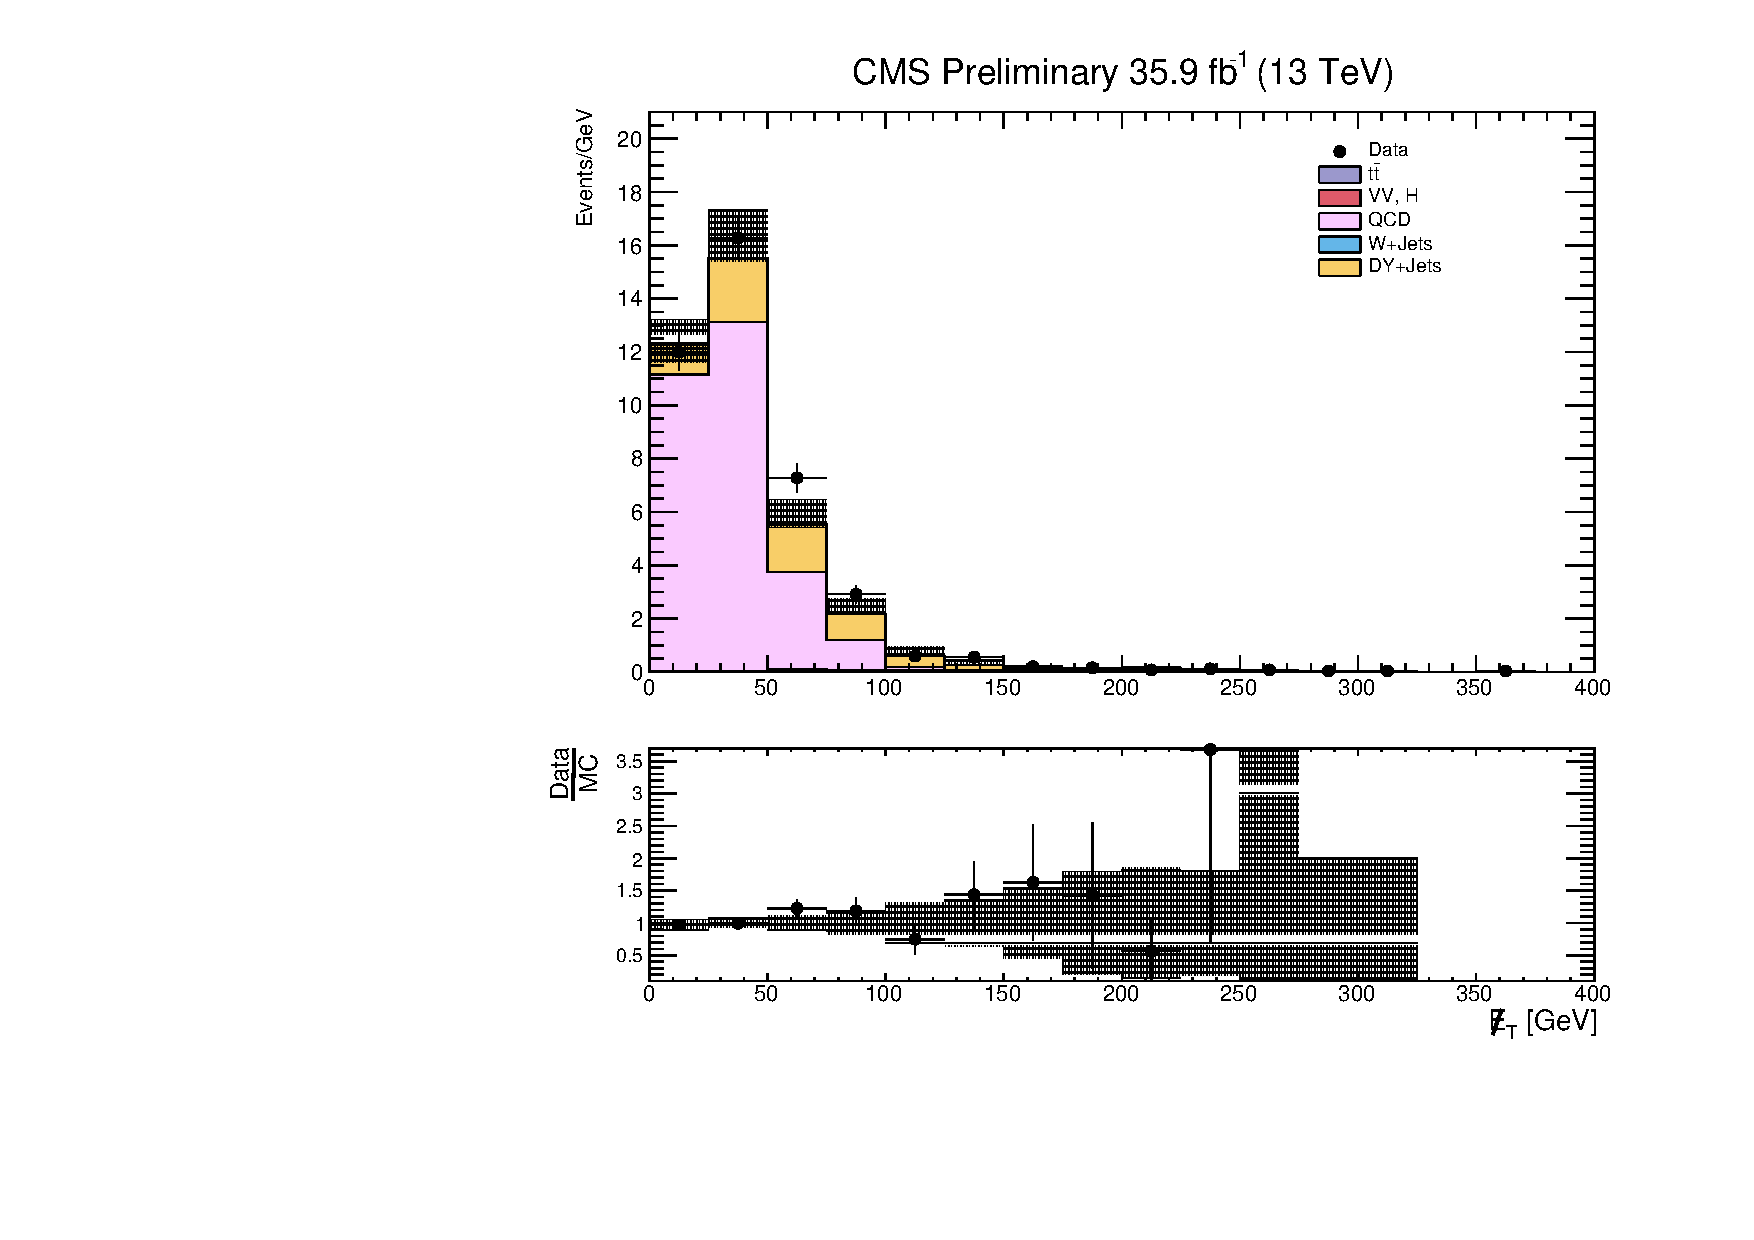
\includegraphics[clip,width=0.46\textwidth]{figuras/Chapter5/NminusOne/noMET.pdf}
%  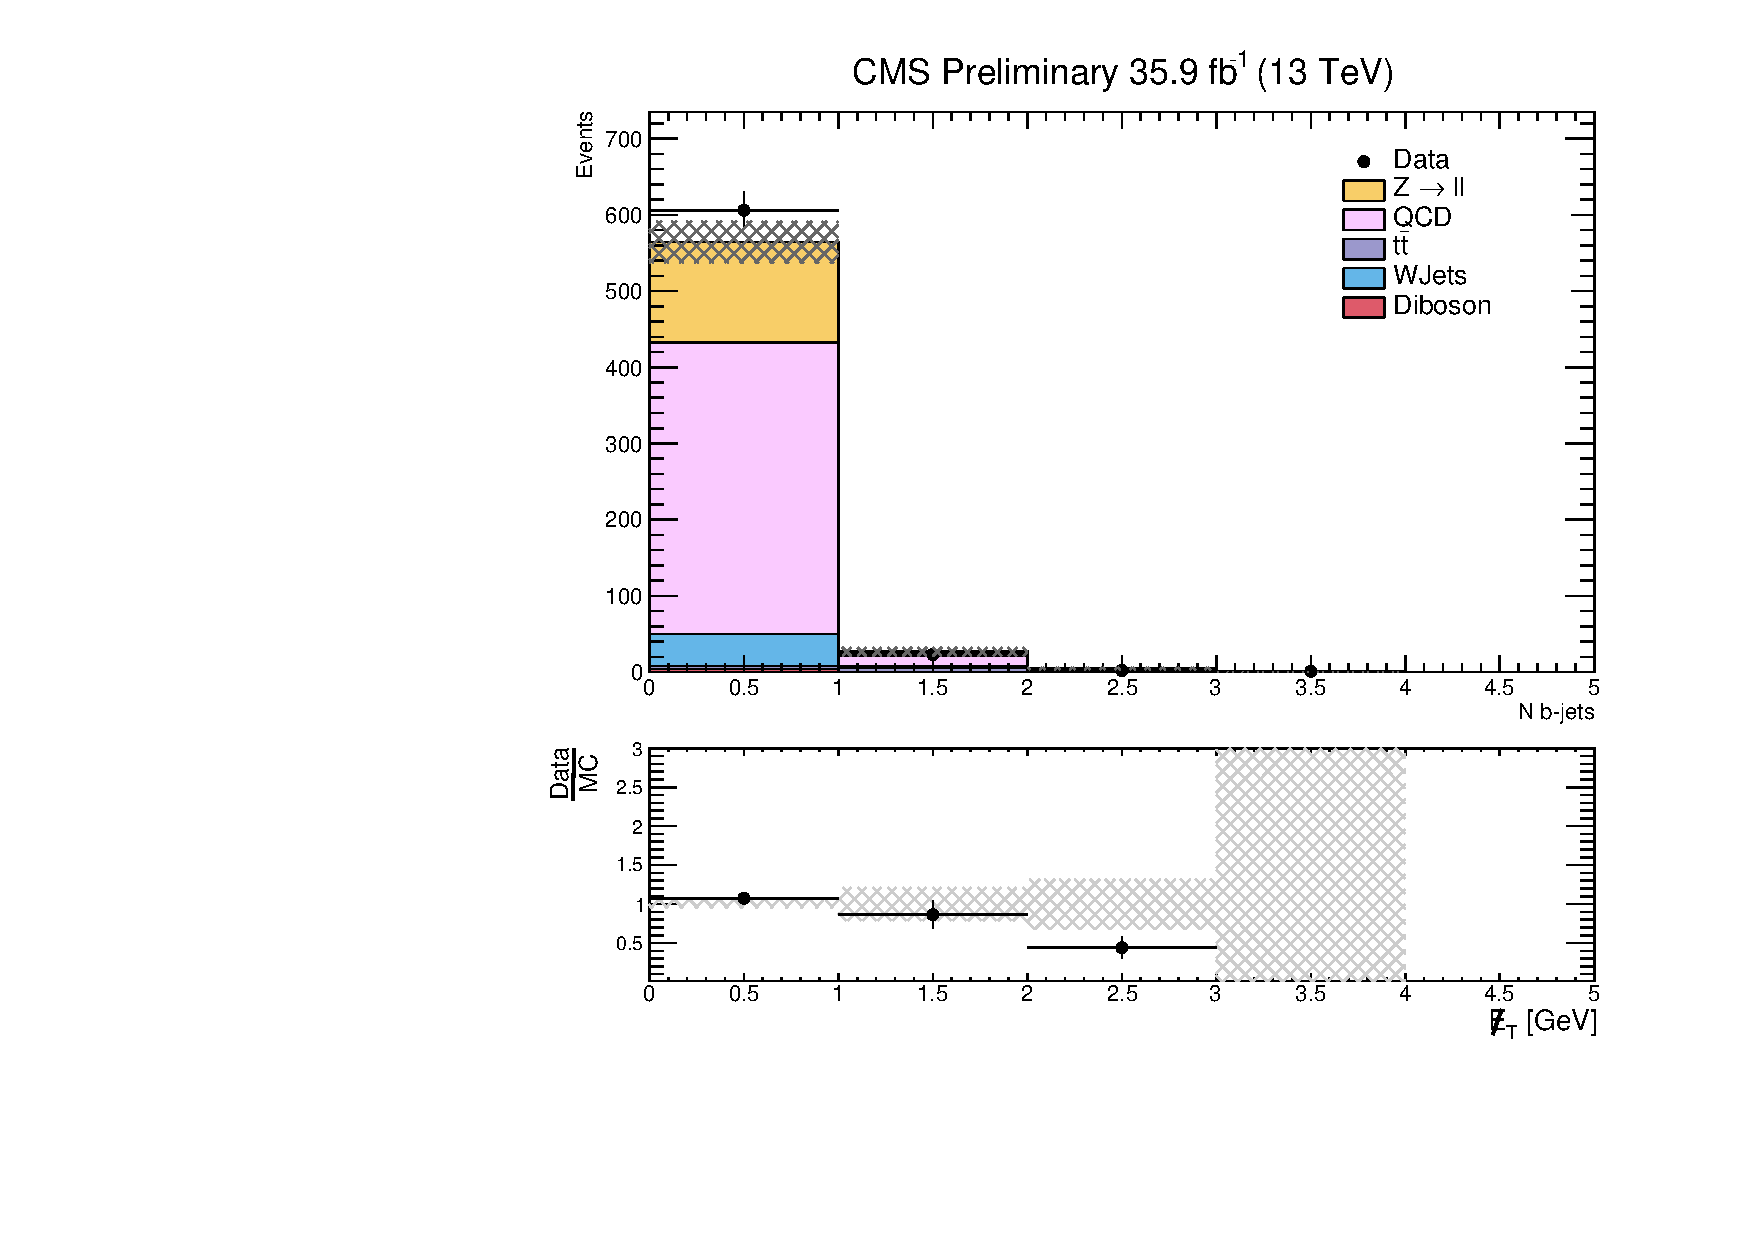
\includegraphics[clip,width=0.46\textwidth]{figuras/Chapter5/NminusOne/noBjet.pdf} }
%  \resizebox{\textwidth}{8.8cm}{
%  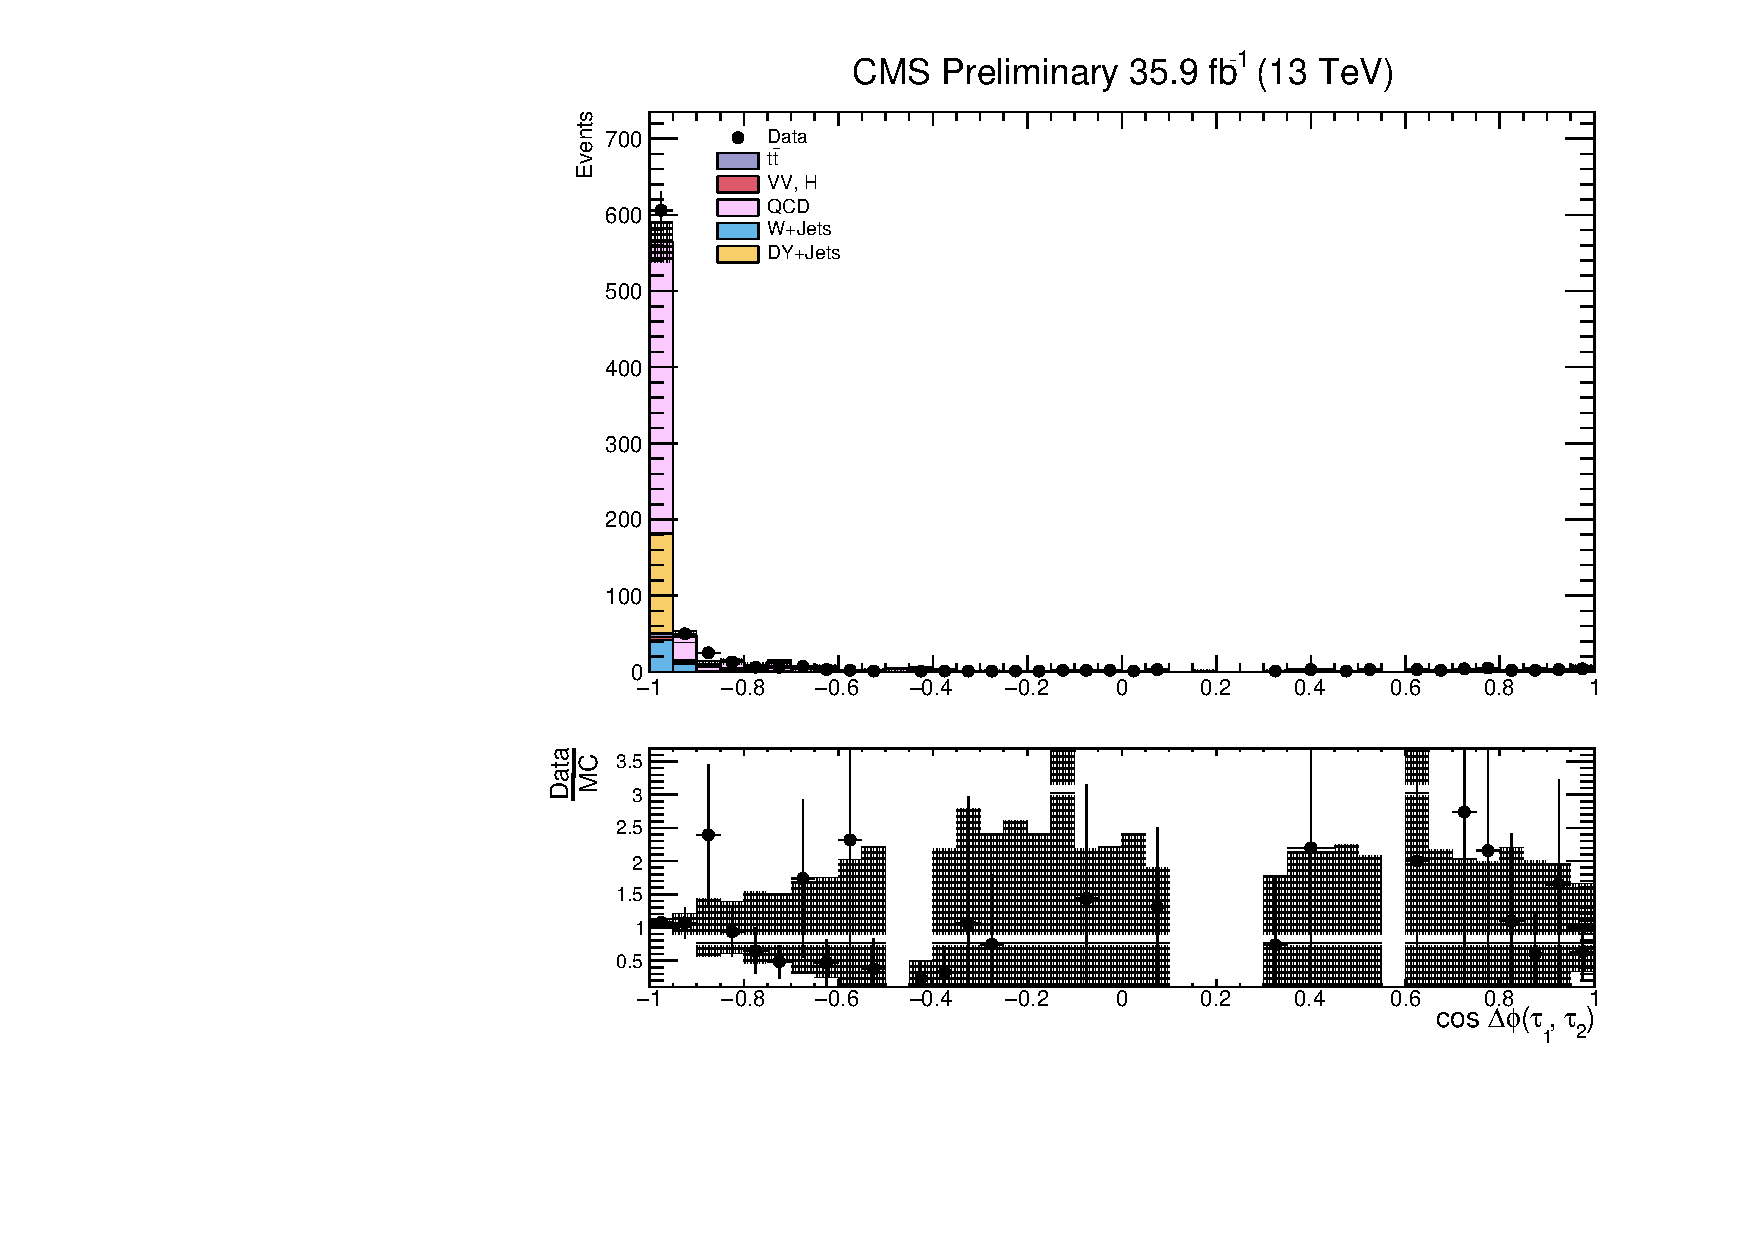
\includegraphics[clip,width=0.46\textwidth]{figuras/Chapter5/NminusOne/noCosDphi.pdf}
%  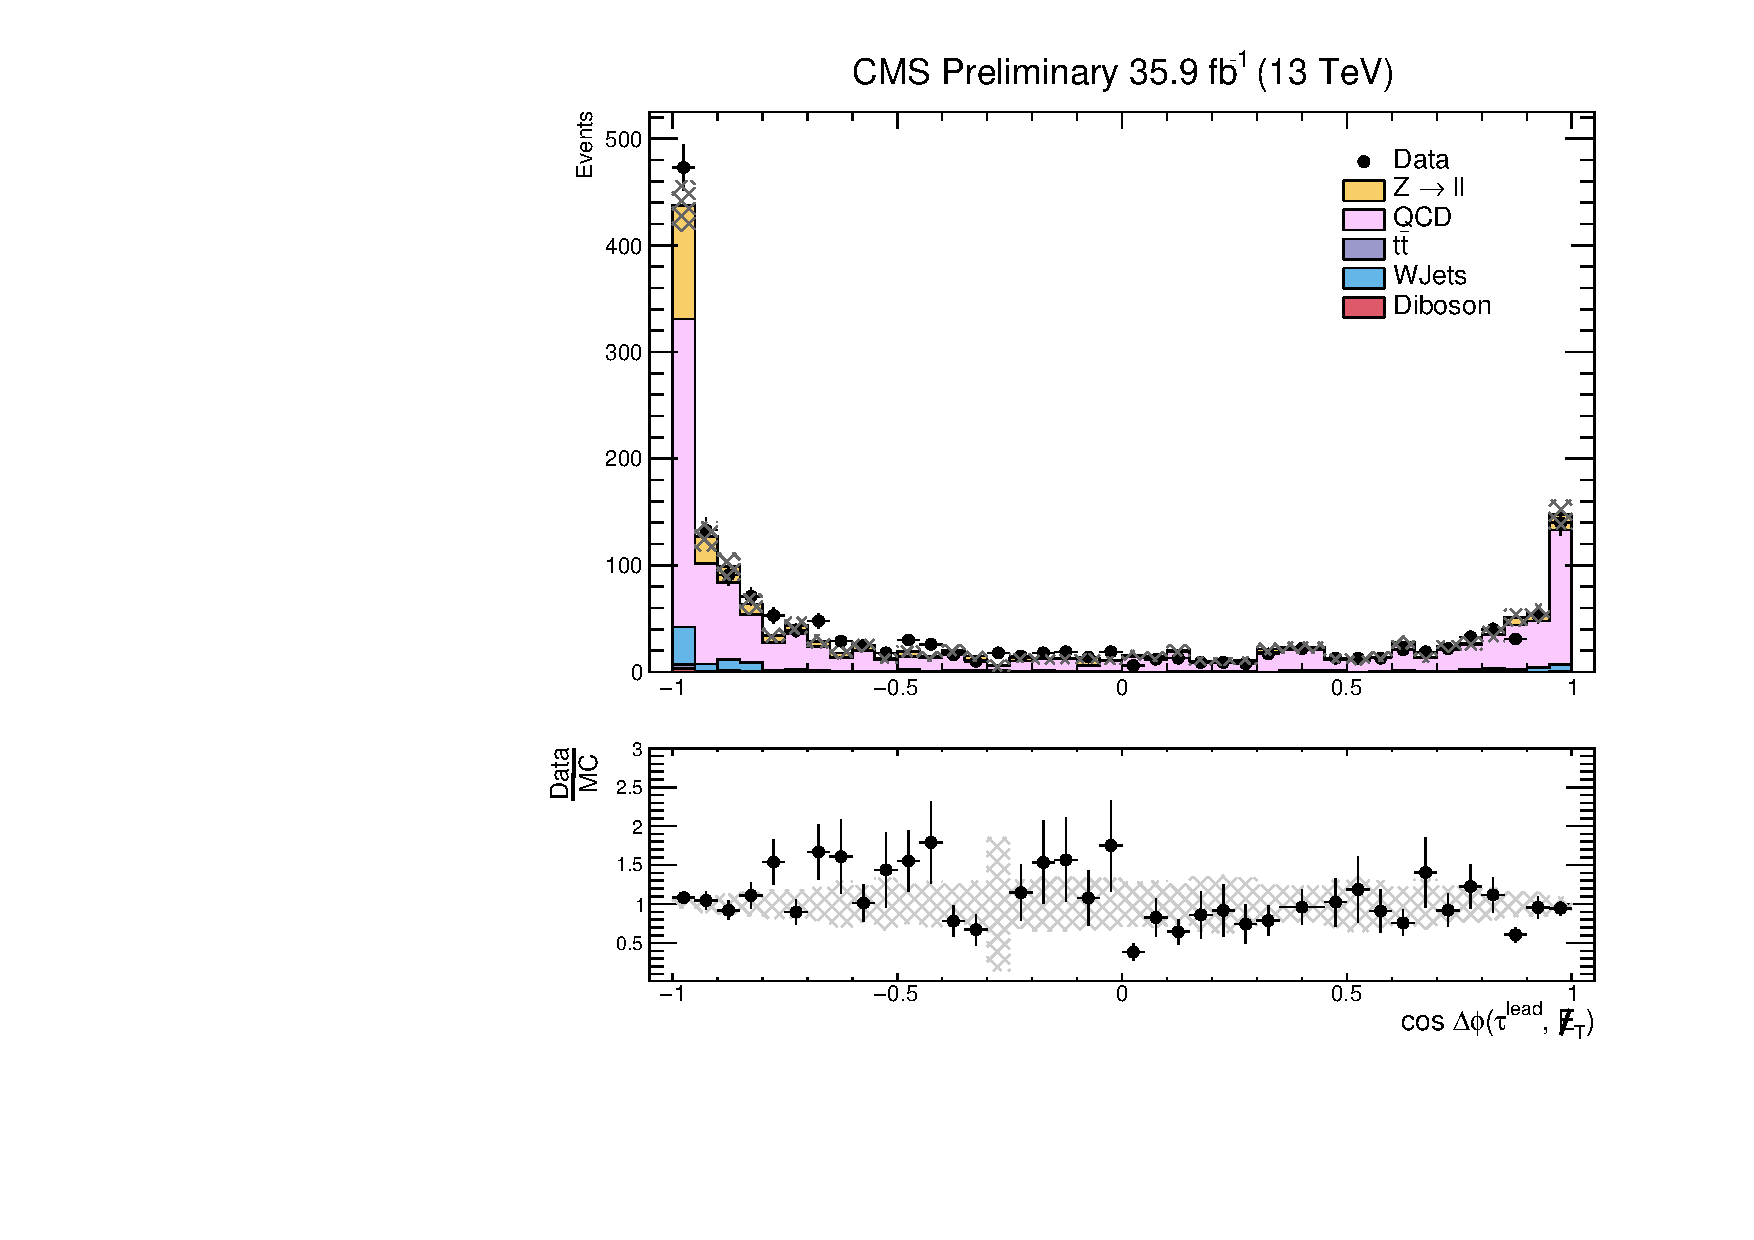
\includegraphics[clip,width=0.46\textwidth]{figuras/Chapter5/NminusOne/noCosDphiTauMET.pdf}}
%  \end{center}
%  \caption{Distribution of variables after all requirements for the signal region with exception of
% one plotted. \MET~(top left), number of b-jets (top right), $\cos\Delta \phi (\tau_{1},\tau_{2})$ (bottom left), $\Delta \phi (\tau_{lead}, \not\!\!E_T)$ (bottom right). 
% QCD background has been estimated with a data-driven method.}
% \label{nminusone} 
%  \end{figure}

 
% \begin{table}
%   \resizebox{\textwidth}{!}{
% 
% \begin{tabular}{ | l | c | c | c | c | c | c | }
% \hline
% Process            & DY+Jets              & QCD                 & VV                & W+Jets                & t#bar{t}             & Zprime3000\\ \hline
% NRecoVertex     & 569341103.9 $\pm$ 76915.2 & -3383777796.0 $\pm$ 3219134020.2 & 3194374.4 $\pm$ 3.2 & 2331078505.0 $\pm$ 0.0 & 26586590.3 $\pm$ 0.0 & 51.2 $\pm$ 0.0 \\ \hline
% NRecoTriggers1  & 569341103.9 $\pm$ 76915.2 & -3622407071.7 $\pm$ 3219134020.2 & 3194374.4 $\pm$ 3.2 & 2331078505.0 $\pm$ 0.0 & 26586590.3 $\pm$ 0.0 & 51.2 $\pm$ 0.0 \\ \hline
% NRecoTau1          & 173397.8 $\pm$ 794.5 & 1550855.7 $\pm$ 0.0 & 9490.2 $\pm$ 46.6 & 588928.9 $\pm$ 1604.2 & 107322.2 $\pm$ 192.5 & 22.0 $\pm$ 0.0 \\ \hline
% NRecoTau2          &   1262.8 $\pm$  40.8 &    9784.1 $\pm$ 0.0 &   65.6 $\pm$  3.4 &    387.7 $\pm$   21.2 &    188.5 $\pm$   8.1 &  3.2 $\pm$ 0.0 \\ \hline
% METCut             &    780.3 $\pm$  32.2 &    4126.0 $\pm$ 0.0 &   49.7 $\pm$  2.9 &    282.2 $\pm$   16.5 &    157.7 $\pm$   7.4 &  3.0 $\pm$ 0.0 \\ \hline
% NRecoBJet          &    653.7 $\pm$  28.9 &    3808.0 $\pm$ 0.0 &   38.8 $\pm$  2.7 &    255.6 $\pm$   16.1 &     36.7 $\pm$   3.6 &  2.7 $\pm$ 0.0 \\ \hline
% % OS + DeltaR        &    564.1 $\pm$  26.5 &    1605.8 $\pm$ 0.0 &   32.8 $\pm$  2.5 &    190.0 $\pm$   13.5 &     27.9 $\pm$   3.1 &  2.3 $\pm$ 0.0 \\ \hline
% CosDphi            &    254.4 $\pm$  13.6 &    1191.7 $\pm$ 0.0 &    9.0 $\pm$  1.7 &    103.3 $\pm$   10.0 &     12.8 $\pm$   2.1 &  2.2 $\pm$ 0.0 \\ \hline
% cosDphiTauMET      &    131.6 $\pm$   8.6 &     382.7 $\pm$ 0.0 &    3.7 $\pm$  1.1 &     41.9 $\pm$    5.2 &      4.4 $\pm$   1.2 &  1.9 $\pm$ 0.0 \\ \hline
% \end{tabular}
% }
%  
% \end{table}
% 



\section{Background Estimation}
\label{sec:BackgroundEstimation}

The main source of background for the di-hadronic tau final state is 
dominated by the probability of misidentifying QCD-jets as taus, where 
di-jets can fake the \Zprimetotauh~signature; this source accounts 
for 70$\%$ of the total background. As can be noted 
in Figure \ref{nminusone_MC}, the QCD MC-samples do
not have enough statistics in order to estimate properly 
the expected SM contamination due to these processes. Additionally, the large uncertainties in 
treating the processes of fragmentation and hadronization that involved in the modeling of QCD-jet 
production, as well as the uncertainties of the pile-up effects and the interaction of the jet products with
the detector material, make QCD MC simulation not reliable. Therefore, the
QCD background contribution must be determined using data-driven methods, based on 
the creation of enriched control samples obtained by modifying the signal selection
criteria. \\

\noindent Another important source of background comes 
from Drell-Yan processes, approximately 23$\%$, 
which have the same topology than the signal. Since these SM 
processes have been extensively studied, two high-quality 
hadronic taus are expected to be well modeled by simulation and, therefore, 
an MC based approach is employed to estimate their contribution 
to the signal region, instead of a data-driven method. In order to 
determine the level of accuracy of the MC backgrounds, 
an enriched \Ztotauh~control sample is defined, where no
considerable fluctuations between data and MC are expected. This control 
sample also allows to validate the tau identification 
criteria used in this analysis.

\subsection{Background Estimation for QCD}
\label{subsec:QCD}

\noindent The QCD contamination expected in the signal region is estimated 
using the so-called ``ABCD method'', where the QCD yield ($N_{SR}^{QCD}$),
as well as the shape and the normalization in the final 
distributions, are obtained from data. The basic idea is to
estimate $N_{SR}^{QCD}$ from a control sample dominated by QCD events; in this case, 
the sample is obtained requiring the same signal 
criteria but selecting \tauh \tauh~pairs with like-sign (LS) electric charge. Assuming 
that the electric charges of both QCD jets are not correlated, the yield of the like-sign 
QCD di-jet events ($N_{LS}^{QCD}$) should be the same 
as the one of oppositely-charged QCD di-jet (OS) events. However,
this assumption cannot be true for events where the charges of the quarks, 
which give rise to the QCD di-jets, are correlated. The quark charge can be 
correlated with the charge of the leading track of the jet; this correlation
is especially strong for jets with low multiplicity of high-momentum tracks, 
which most likely can fake the tau signature. In consequence, if the two quarks
are kinematically correlated, for instance through $q\bar{q}$ production, that can 
result in an oppositely-charged QCD di-jet event, that could fake a $\tau^{+}\tau^{-}$
event. This leads to an asymmetry between $N_{SR}^{QCD}$ 
and $N_{LS}^{QCD}$ and, therefore, a normalization factor must be included in the $N_{SR}^{QCD}$ estimation. 
Thus, the QCD yield in the signal region is given by:

\begin{equation}
 N_{SR}^{QCD} = R_{OSLS} \times N_{LS}^{QCD}\; ,
\end{equation}

\noindent where $R_{OSLS}$ is the normalization factor, which represents
the $N_{OS}^{QCD} / N_{LS}^{QCD}$ asymmetry.\\

\noindent In order to estimate the $OS/LS$ ratio, other enriched QCD control regions 
are defined. As was mentioned in the previous section (see Figure \ref{MET}), the 
\MET~$<$ 30 \GeV~region is highly contaminated by QCD events and, therefore,
it can be used to measure the $OS/LS$ ratio; with this purpose, the \MET~$<$ 30 \GeV~sideband
is split into two control regions: one composed by oppositely-charged di-jet
events and, the other one, by like-sign di-jet events. Figure \ref{fig:QCD_Strategy} shows the 
overview of the data-driven ``ABCD method'' used to estimate the 
QCD contribution in the signal region.\\

\noindent In summary, the shape of the \mass~distribution in the 
signal region is obtained from the control region C, which consists
in like-sign di-jet events and \MET~$>$ 30 \GeV. The distribution
is normalized to the contribution of oppositely-charged QCD di-jet,
using the $OS/LS$ ratio. The ratio is measured using control regions B 
and D (\MET~$<$ 30 \GeV~sideband) as follows:
 
 \begin{equation} \label{eq:ratio}
  R_{OSLS} = \frac{N_{B}^{QCD}}{N_{D}^{QCD}} \; .
 \end{equation}

\begin{figure}[H]
 \begin{center}
 \captionsetup[subfloat]{farskip=0pt,captionskip=0.0cm,labelformat=empty}
 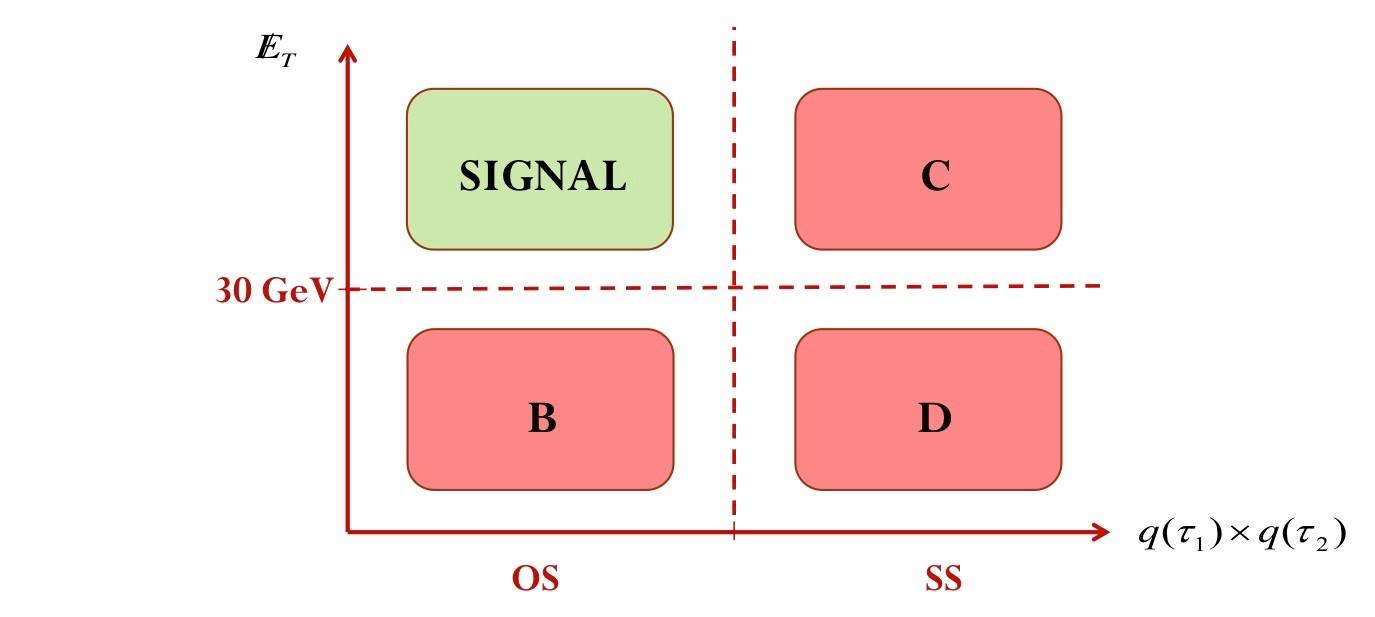
\includegraphics[clip,width=0.7\textwidth]{figuras/Chapter5/QCD_Estimation/QCD_Strategy}
  \end{center}
 \caption{Overview of the data-driven method to estimate the QCD background.}
\label{fig:QCD_Strategy} 
 \end{figure}

%  Note that three 
% control regions dominated by QCD (B, C, and D) were defined

\noindent As was mentioned, control regions B, C and D are dominated by QCD
and simulated samples cannot be used to predict this background. Then, 
any disagreement between data and the other expected SM processes
in these control regions is assigned to QCD events. This means that
the QCD estimation is obtained from data by subtracting any 
contribution coming from non-QCD processes, such as DY, W+Jets, DiBoson and $t\bar{t}$. In consequence:

\begin{equation} \label{eq:QCD}
\begin{split}
 N_{B}^{QCD} &= N_{B}^{Data} - N_{B}^{nonQCD}\; , \\
 N_{C}^{QCD} &= N_{C}^{Data} - N_{C}^{nonQCD}\; , \\
 N_{D}^{QCD} &= N_{D}^{Data} - N_{D}^{nonQCD}\; . \\
\end{split}
\end{equation}

\noindent Thus, in order to measure the $OS/LS$ ratio using the equation \ref{eq:ratio},
the QCD estimation was performed in control regions B and D,
considering the equations \ref{eq:QCD}. Table \ref{tab:ratio} shows the data 
and MC yields in these controls regions. Note that the QCD estimation  presented 
in the table corresponds to $Data-nonQCD$. The purity of the QCD samples obtained
in the control regions B and D, defined as $(Data-nonQCD)/Data$, 
is 85$\%$ and 99$\%$, respectively. On the other hand, the contamination
from signal in these control regions is less than 0.01$\%$ since any \Zprime~boson events
are expected to have \MET~greater than 30 \GeV. Since a high QCD purity and low 
signal contamination is obtained, these control regions are appropriated
to estimate the $OS/LS$ ratio. The $OS/LS$ ratio resulted from this procedure 
was 1.34 $\pm$ 0.12. Figure \ref{fig:ratio} shows that the measured $OS/LS$ ratio 
can be considered as a constant in the effective mass spectrum.\\

\begin{tiny} 
 \begin{table}[ht] 
 \centering{ 
 \begin{tabular}{ | l | r | r |} \hline \hline 
   &  \textbf{CR B Yields}   & \textbf{CR D Yields} \\ \hline \hline 
 \textbf{Data}         & \textbf{405.00  $\pm$  20.12}    & \textbf{261.00  $\pm$  16.16} \\ \hline 
 DY         & 46.88   $\pm$   6.82  & 0.13   $\pm$   0.07 \\ \hline 
 WJets      & 10.75   $\pm$   6.29  & 1.32   $\pm$   0.93 \\ \hline 
 DiBoson    & 0.62   $\pm$   0.40  & 0.15   $\pm$   0.09 \\ \hline 
 \ttbar     & 0.56   $\pm$   0.44  & 0.34   $\pm$   0.34 \\ \hline 
 \textbf{nonQCD BKG} & \textbf{ 58.82   $\pm$  9.30}  & \textbf{ 261.00  $\pm$ 16.22} \\ \hline 
 Data - nonQCD & 346.18   $\pm$   22.17  & 259.06   $\pm$   16.19 \\ \hline  \hline
 TOTAL BKG & 405.00   $\pm$   24.04  & 261.00   $\pm$   16.22 \\ \hline  \hline
 \textcolor{blue}{$R_{OSLS}$} & \multicolumn{2}{|c|}{\textcolor{blue}{1.34     $\pm$   0.12}} \\ \hline  \hline
 \end{tabular} 
 } 
   \caption{Yields in the controls region B and D used for calculation of $R_{OSLS}$ ratio.}
  \label{tab:ratio}
 \end{table} 
 \end{tiny}

 \begin{figure}[ht]
 \begin{center}
 \captionsetup[subfloat]{farskip=0pt,captionskip=0.0cm,labelformat=empty}
 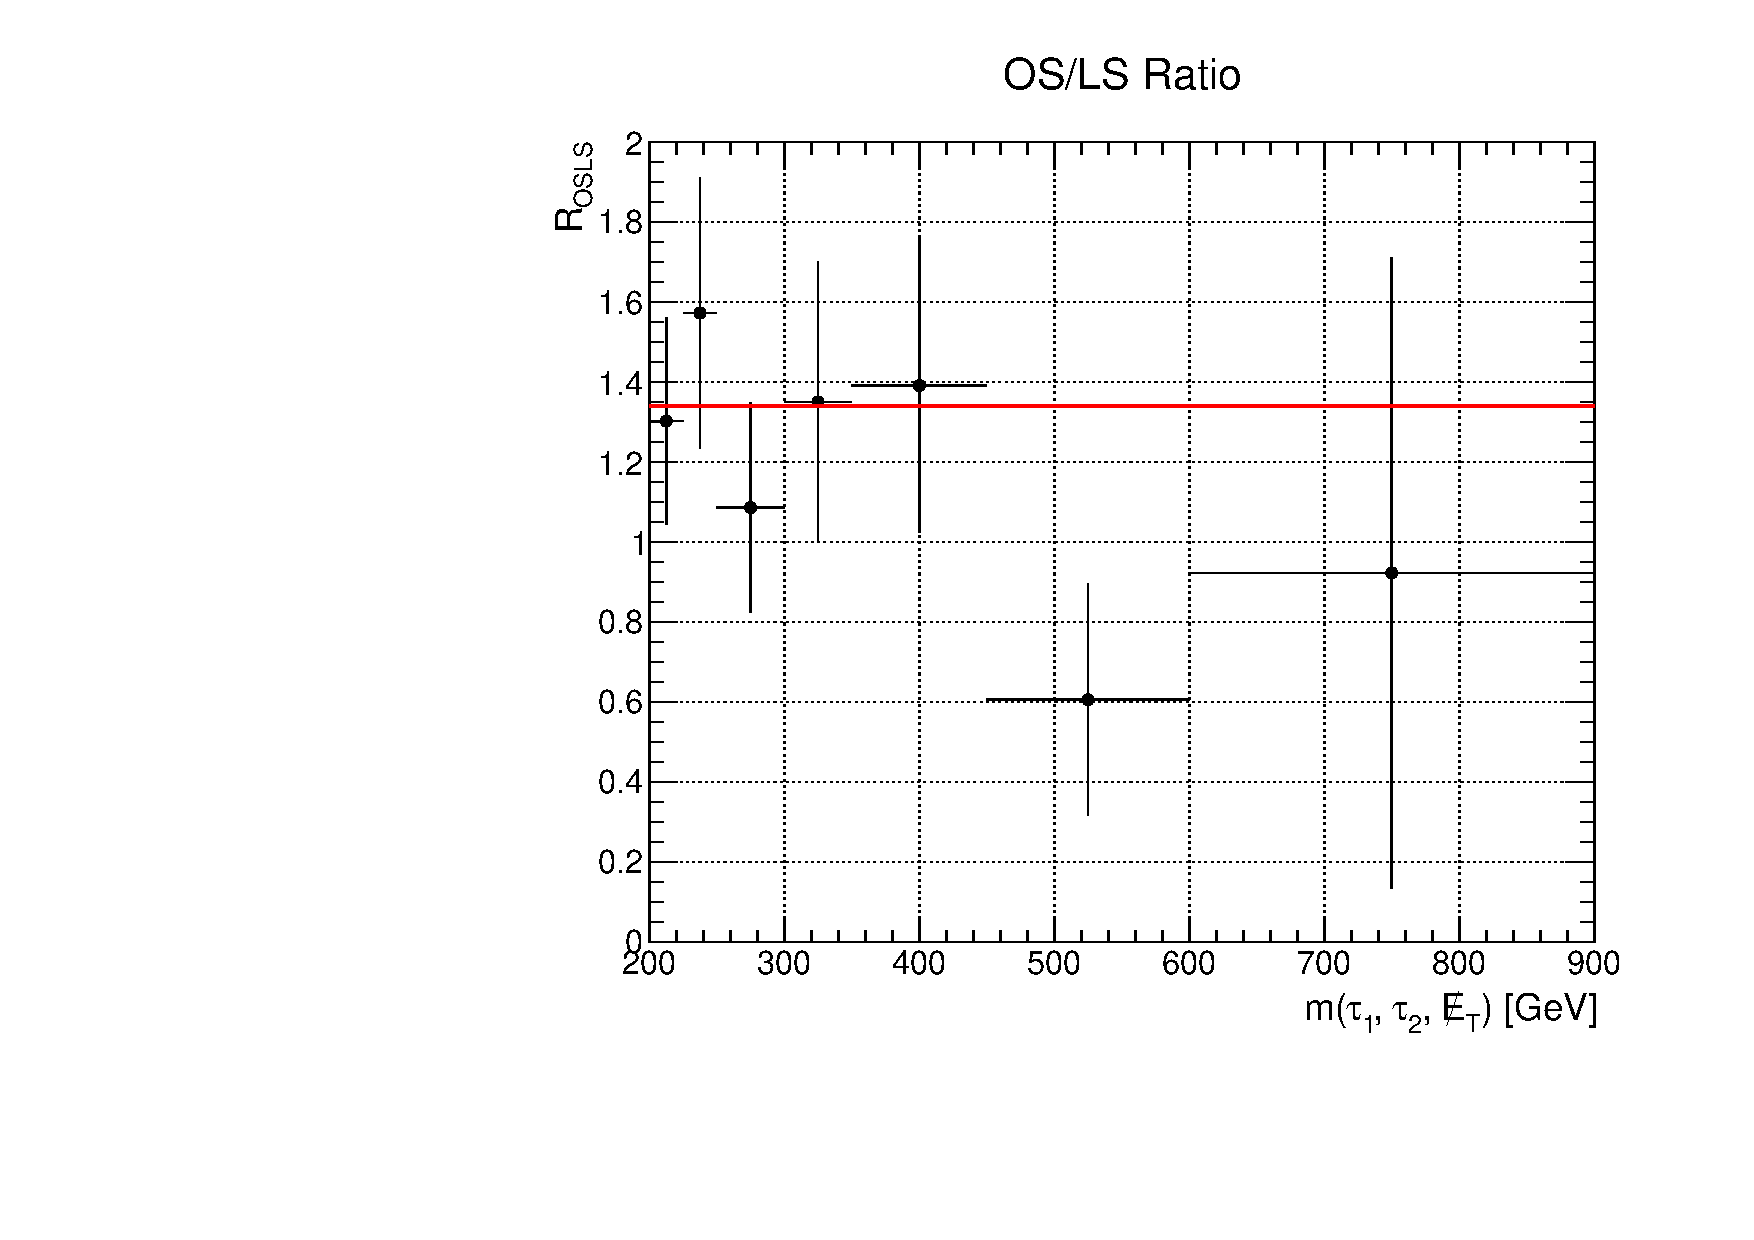
\includegraphics[clip,width=0.5\textwidth]{figuras/Chapter5/QCD_Estimation/OSLS_Ratio_1p34.pdf}
 \end{center}
 \caption{The measured $OS/LS$ ratio in function of the effective mass.}
  \label{fig:ratio}	
 \end{figure}
 
\noindent The normalization and the determination of the 
\mass~shape must be tested in order to validate 
the QCD estimation in the signal region. Nevertheless, since 
the QCD simulated samples do not have enough statistics,
the validation must be performed using real data. Then, a test 
is performed to check simultaneously the 
proper normalization (usually known as closure test) and 
to validate if the \mass~shape in the opposite-sign regions can be modeled 
correctly by like-sign di-hadronic taus events. In order 
to perform the shape closure/validation test, the QCD background 
is estimated in the control region B from the \mass~shape 
obtained in the control region D (like-sign region), and the correct 
normalization is obtained using the $OS/LS$ ratio. \\


\noindent The agreement between the data and the expected background in the effective
mass spectrum determines if the QCD \mass-shape in the oppositely-charged
taus region can be well modeled from the like-sign region. In case in which
there would be a disagreement, a systematic uncertainty on the shape could be included in 
the final results. As can be seen in Figure \ref{fig:CR_B}, there is a 
good data$/$background agreement and, therefore, no systematic uncertainties were 
applied due to the shape of the QCD estimation; additionally, this agreement 
implies that the same method can be used to estimate QCD background in the signal region.\\
 
 \begin{figure}[ht]
 \begin{center}
 \captionsetup[subfloat]{farskip=0pt,captionskip=0.0cm,labelformat=empty}
 \resizebox{\textwidth}{8.8cm}{
 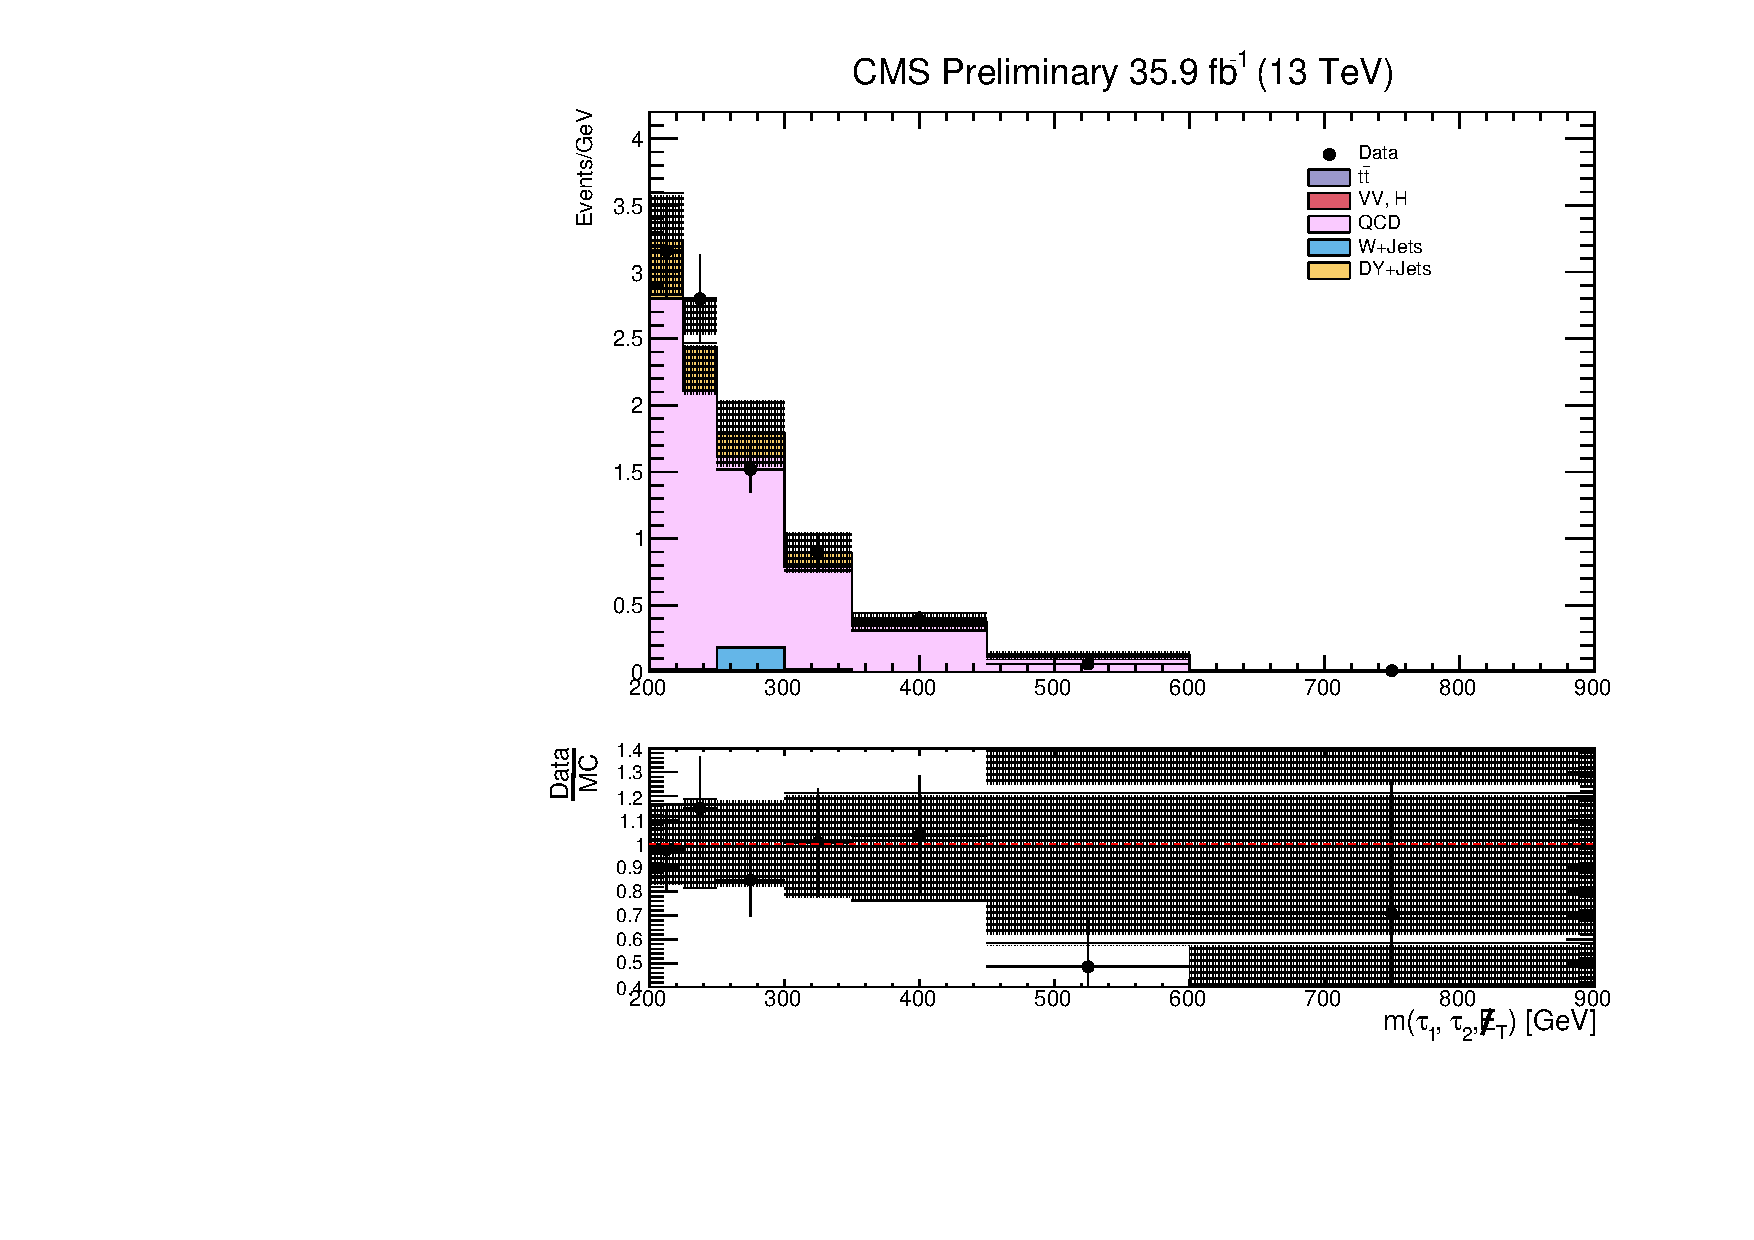
\includegraphics[clip,width=0.45\textwidth]{figuras/Chapter5/QCD_Estimation/CR_B.pdf}
 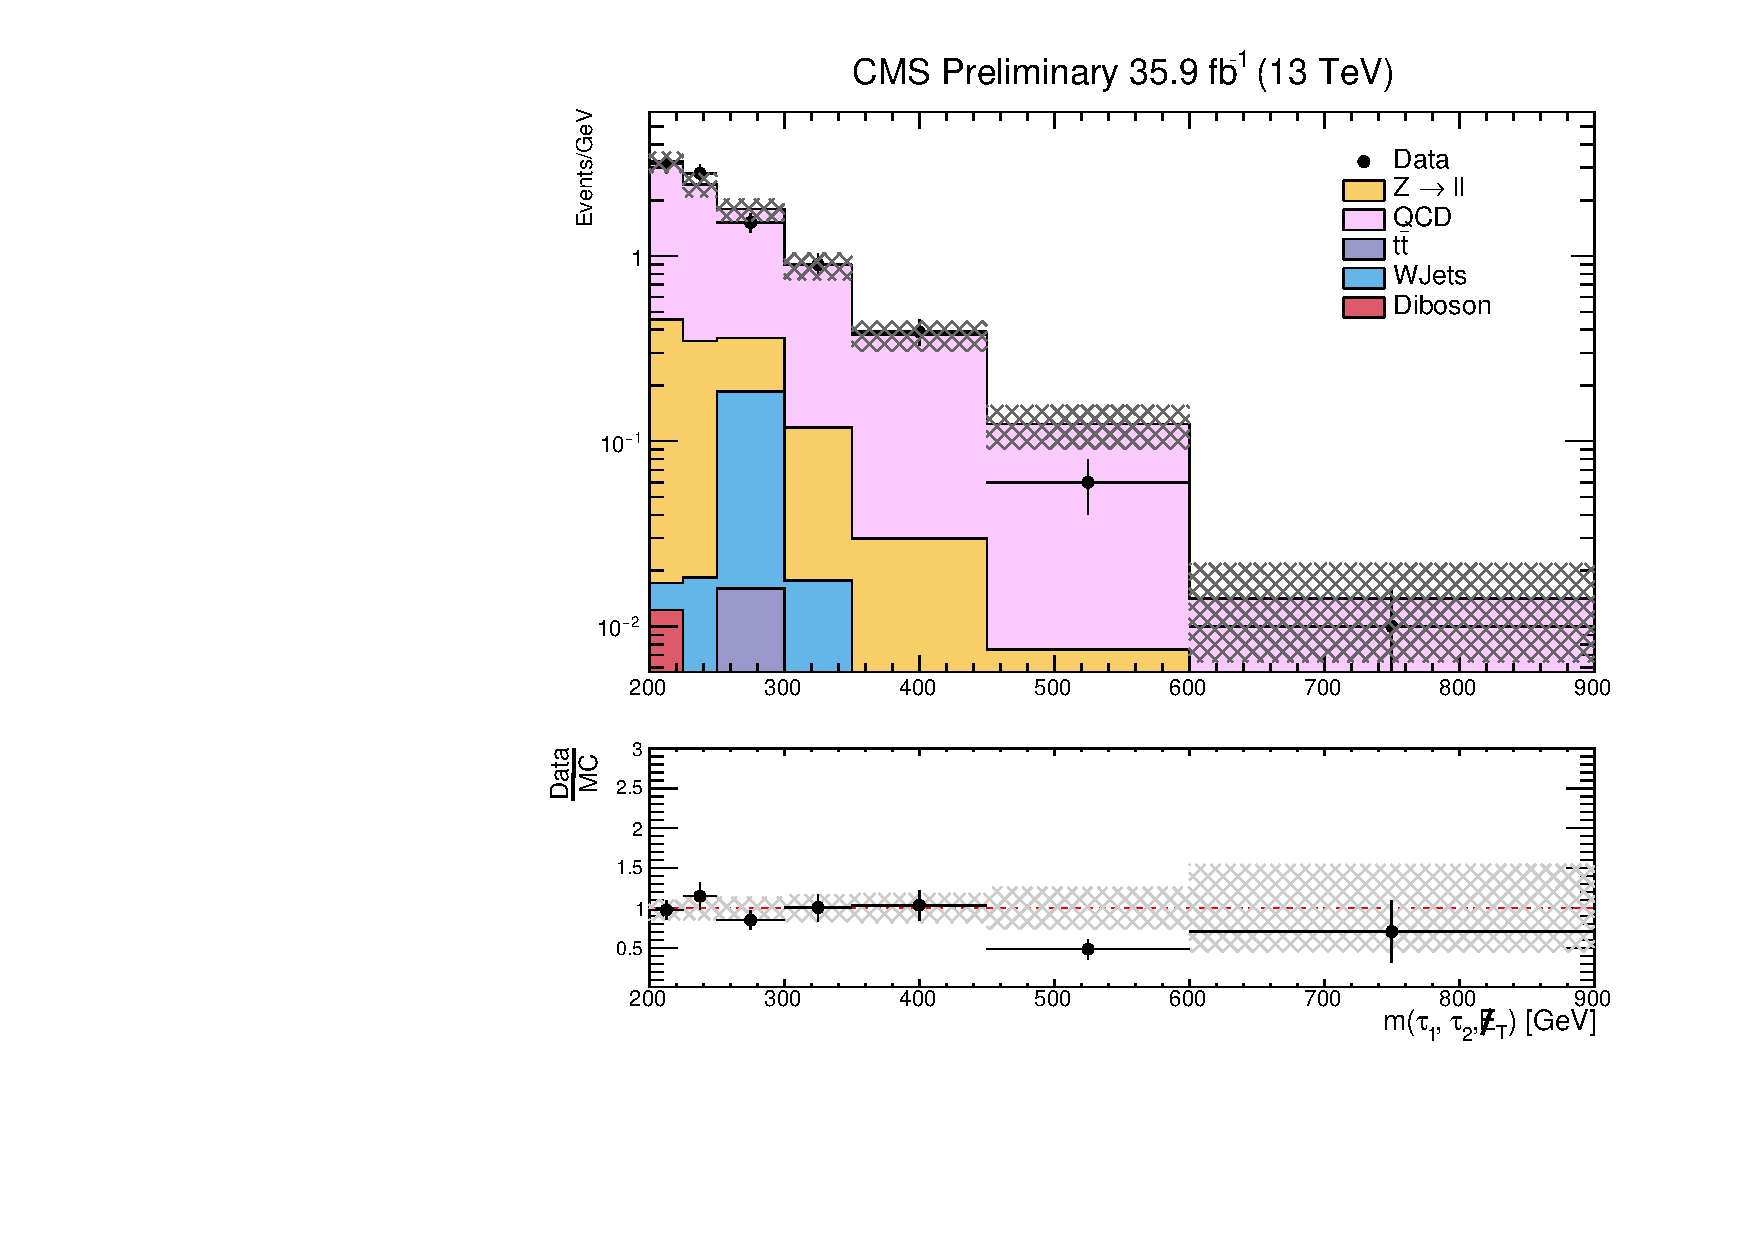
\includegraphics[clip,width=0.45\textwidth]{figuras/Chapter5/QCD_Estimation/CR_B_log.pdf}
 }
 \end{center}
 \caption{\mass~distribution in OS tau-pairs with low-\MET~(control region B): Normal scale (left),
 and log scale (right). QCD background was estimated from SS events in the 
 low-\MET~sideband (control region D), normalized to QCD estimation in control region B 
 using the $R_{OSLS}$ ratio. Only the statistical uncertainties have been included.}
  \label{fig:CR_B}
 \end{figure}
 
\noindent Table \ref{tab:signalregion} shows the amount of events coming from each
background contamination in the signal region, as well as the yield of 
data and background in the control region C. The QCD background in the signal 
region is estimated using the same method described above, which consists of taking the \mass~shape
from the like-signal di-hadronic tau events ($Data^{C} - nonQCD^{C}$) and normalizing
it using the $OS/LS$ ratio. The table also shows the expected signal events in the signal 
region, as well as the contamination due to the signal in the control region C (1.6$\%$). Table \ref{tab:QCDBGEstimationTable} shows 
the QCD yield estimated in each control region. The final prediction of this background in the signal region 
is 382.67 $\pm$ 24.84 (right-most column of the table), where the uncertainty
is fully statistical. The QCD purity in the signal region, 
defined as $(Data^{C}-nonQCD^{C})/Data^{C}$, is 85$\%$ for effective 
masses above 600 \GeV~(see Figure \ref{fig:QCDpurity}), where 
the signal is expected.\\

\noindent The other backgrounds in Table \ref{tab:signalregion} were estimated from 
simulated samples. As was mentioned before, the estimation of Drell-Yan processes, 
which represents around 23$\%$ of the total background in the signal region,
is validated using a $Z \rightarrow \tau\tau$ control region (see next section). 
The remaining processes (W+Jets, \ttbar~and DiBoson), which represent only  
8$\%$ of the background, are also estimated from simulated samples. \\

\noindent Figure \ref{fig:SR_Result} shows the \mass~distribution in the 
signal region. This distribution represents the most important plot for this analysis, since if a 
\Zprime~exists it would show up as a broad resonance in the high effective 
mass spectrum, as can be seen in the figure. Then, once the 
background estimation performed is validated (see Section \ref{subsec:Validation}), 
the signal selection criteria are applied on real data samples and
any excess in the \mass~distribution over the SM expectation 
could represent the existence of a \Zprime~boson. 
% \vspace{-0.1cm}

\begin{tiny}
  \begin{table}[H] 
 \centering{ 
 \begin{tabular}{ | l | r | r |} \hline \hline 
   &  \textbf{SR YIELDS}   & \textbf{CR C YIELDS} \\ \hline \hline 
 \textbf{Data}         & $---$    & \textbf{314.00  $\pm$  17.72} \\ \hline 
 DY           & 131.61   $\pm$   8.64  & 14.79   $\pm$   4.65 \\ \hline 
 WJets      & 41.91   $\pm$   5.17  & 11.65   $\pm$   2.73 \\ \hline 
 DiBoson    & 3.73   $\pm$   1.07  & 0.94   $\pm$   0.47 \\ \hline 
 \ttbar     & 4.39   $\pm$   1.23  & 1.04   $\pm$   0.60 \\ \hline 
%  \textbf{ nonQCD BKG } & \textbf{ 181.63   $\pm$  10.20}  & \textbf{ 28.42  $\pm$ 5.45} \\ \hline 
 QCD estimation & 382.67   $\pm$   24.84 & 285.58   $\pm$   18.54 \\ \hline  \hline
 TOTAL BKG & 564.30   $\pm$   10.20  & 314.00   $\pm$   19.32 \\ \hline  \hline
 
 Z$'$(1500 \GeV)  & 73.83   $\pm$   0.71 & 5.06   $\pm$   0.19 \\ \hline 
 Z$'$(2000 \GeV)  & 19.55   $\pm$   0.18 & 1.71   $\pm$   0.05 \\ \hline 
 Z$'$(2500 \GeV)  & 5.60    $\pm$   0.05 & 0.63   $\pm$   0.02 \\ \hline 
 Z$'$(3000 \GeV)  & 1.91    $\pm$   0.02 & 0.24   $\pm$   0.01 \\ \hline 
%  Z$'$(3500 \GeV)  & 0.68    $\pm$   0.01 & 0.10   $\pm$   0.00 \\ \hline \hline
%  \textcolor{blue}{$R_{OSLS}$} & \multicolumn{2}{|c|}{\textcolor{blue}{1.34     $\pm$   0.09}} \\ \hline 
 \end{tabular} 
 } 
    \caption{Signal and background yields in signal region and control region C.}
  \label{tab:signalregion}
 \end{table} 
\end{tiny}

 \begin{figure}[H]
 \begin{center}
 \captionsetup[subfloat]{farskip=0pt,captionskip=0.0cm,labelformat=empty}
 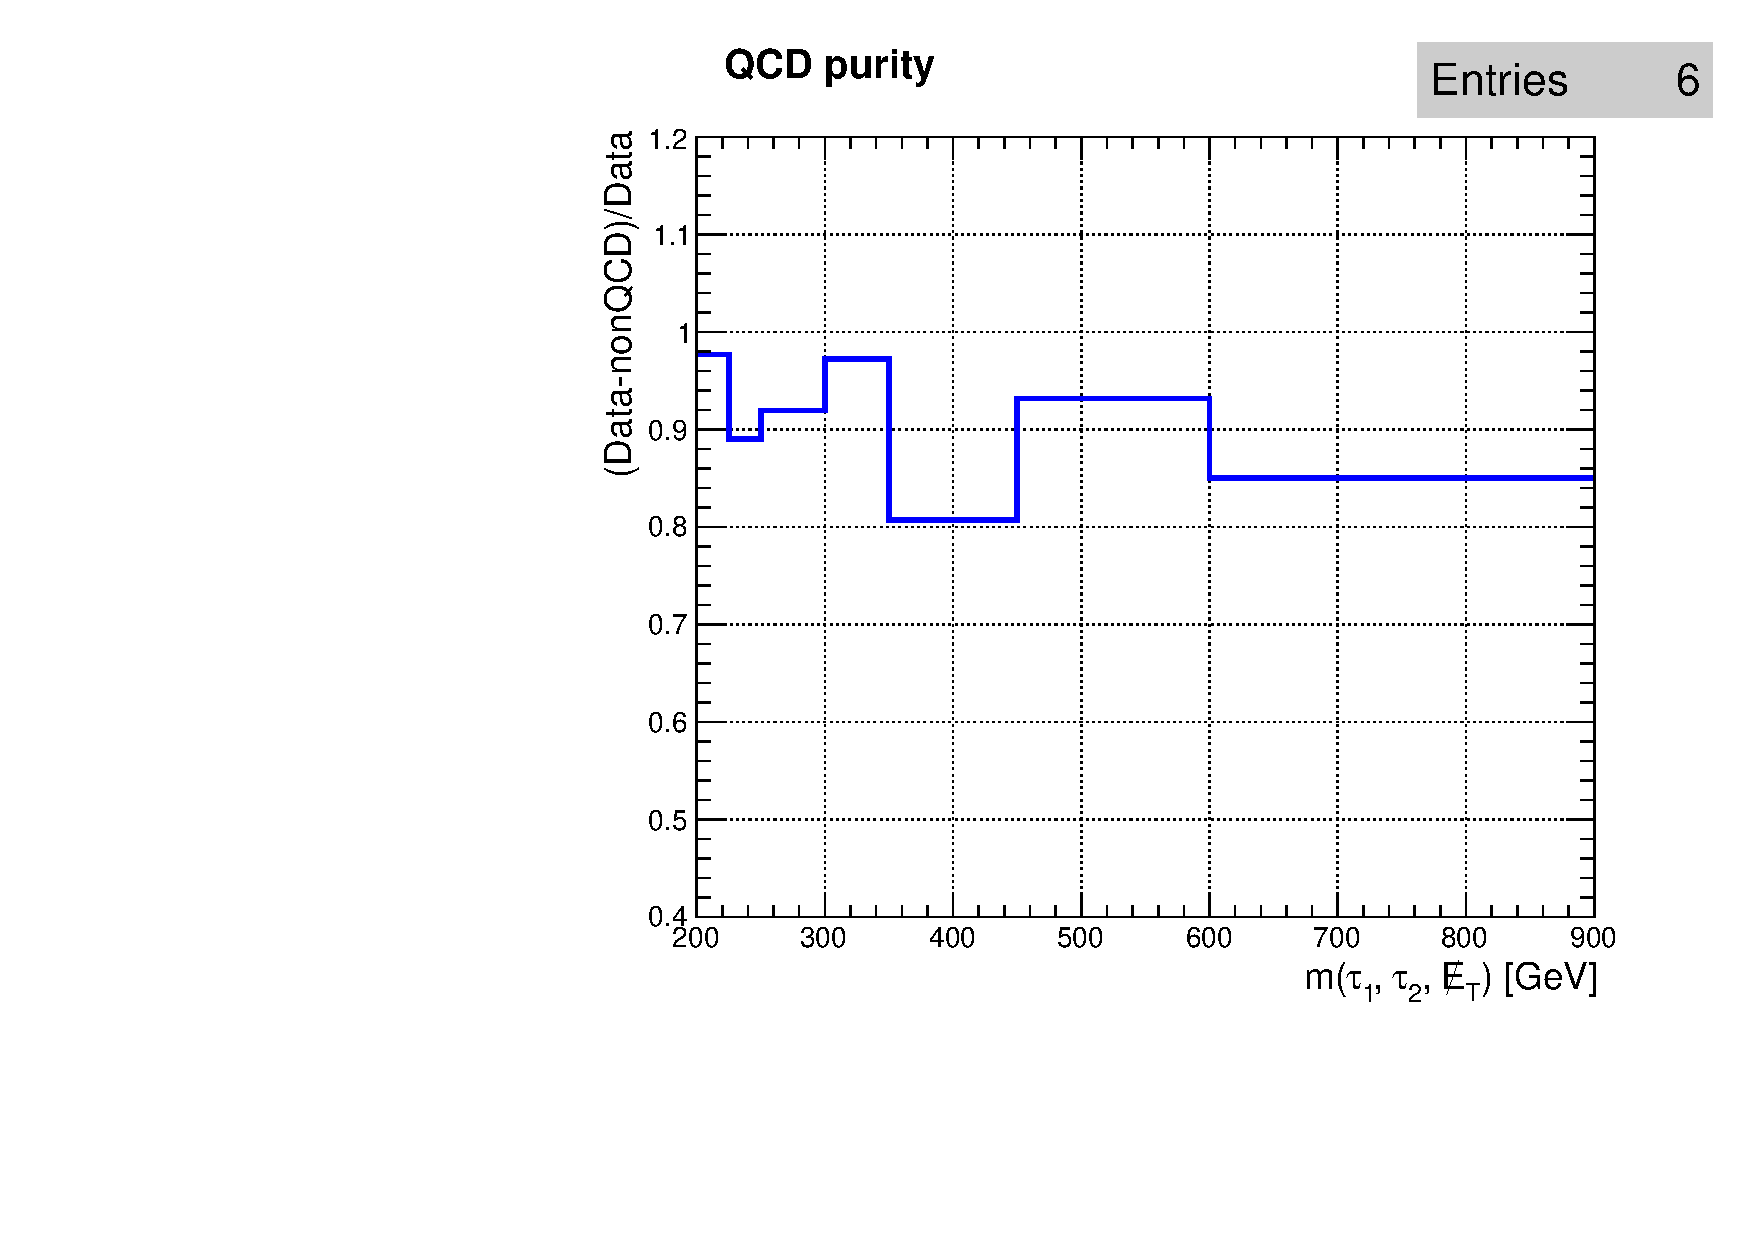
\includegraphics[clip,width=0.45\textwidth]{figuras/Chapter5/QCD_Estimation/QCD_purity.pdf}
 \end{center}
  \caption{QCD purity in the mass spectra of the signal region.}
  \label{fig:QCDpurity}	
 \end{figure}

\noindent Figure \ref{fig:SignalRegionPlots} shows other distributions obtained 
after applying the signal selection criteria (where the QCD background 
was estimated using the data-driven method).


\begin{table}[ht]
\begin{center}
\begin{tabular}{ | l | c | c | c | c | }
\hline \hline
\multirow{2}{*}{\shortstack[c]{Region}}              & \multicolumn{2}{|c|}{\MET~$<$ 30 \GeV~sideband} & \multicolumn{2}{|c|}{\MET~$>$ 30 \GeV~sideband} \\ \cline{2-5}
                                                     & LS $\tau_{h}\tau_{h}$  & OS $\tau_{h}\tau_{h}$  & LS $\tau_{h}\tau_{h}$   & OS $\tau_{h}\tau_{h}$  \\ \hline
QCD         & 259.06 $\pm$ 16.19 & 346.18 $\pm$ 22.17 & 285.58 $\pm$ 18.54 & 382.67 $\pm$ 24.84  \\ \hline \hline
Total BG    & 261.00 $\pm$ 16.22 & 405.00 $\pm$ 24.04 & 314.00 $\pm$ 19.32 & 564.30 $\pm$ 10.20  \\ \hline \hline
\end{tabular} 
\end{center}
  \caption{QCD yields in signal region and in control regions B, C, and D.}
  \label{tab:QCDBGEstimationTable}
\end{table}




% The results are shown 
% in Chapter \ref{chap:Conclusions}. \\

 \begin{figure}[H]
 \begin{center}
  \captionsetup[subfloat]{farskip=0pt,captionskip=0.0cm,labelformat=empty}
%  \resizebox{\textwidth}{!}{
 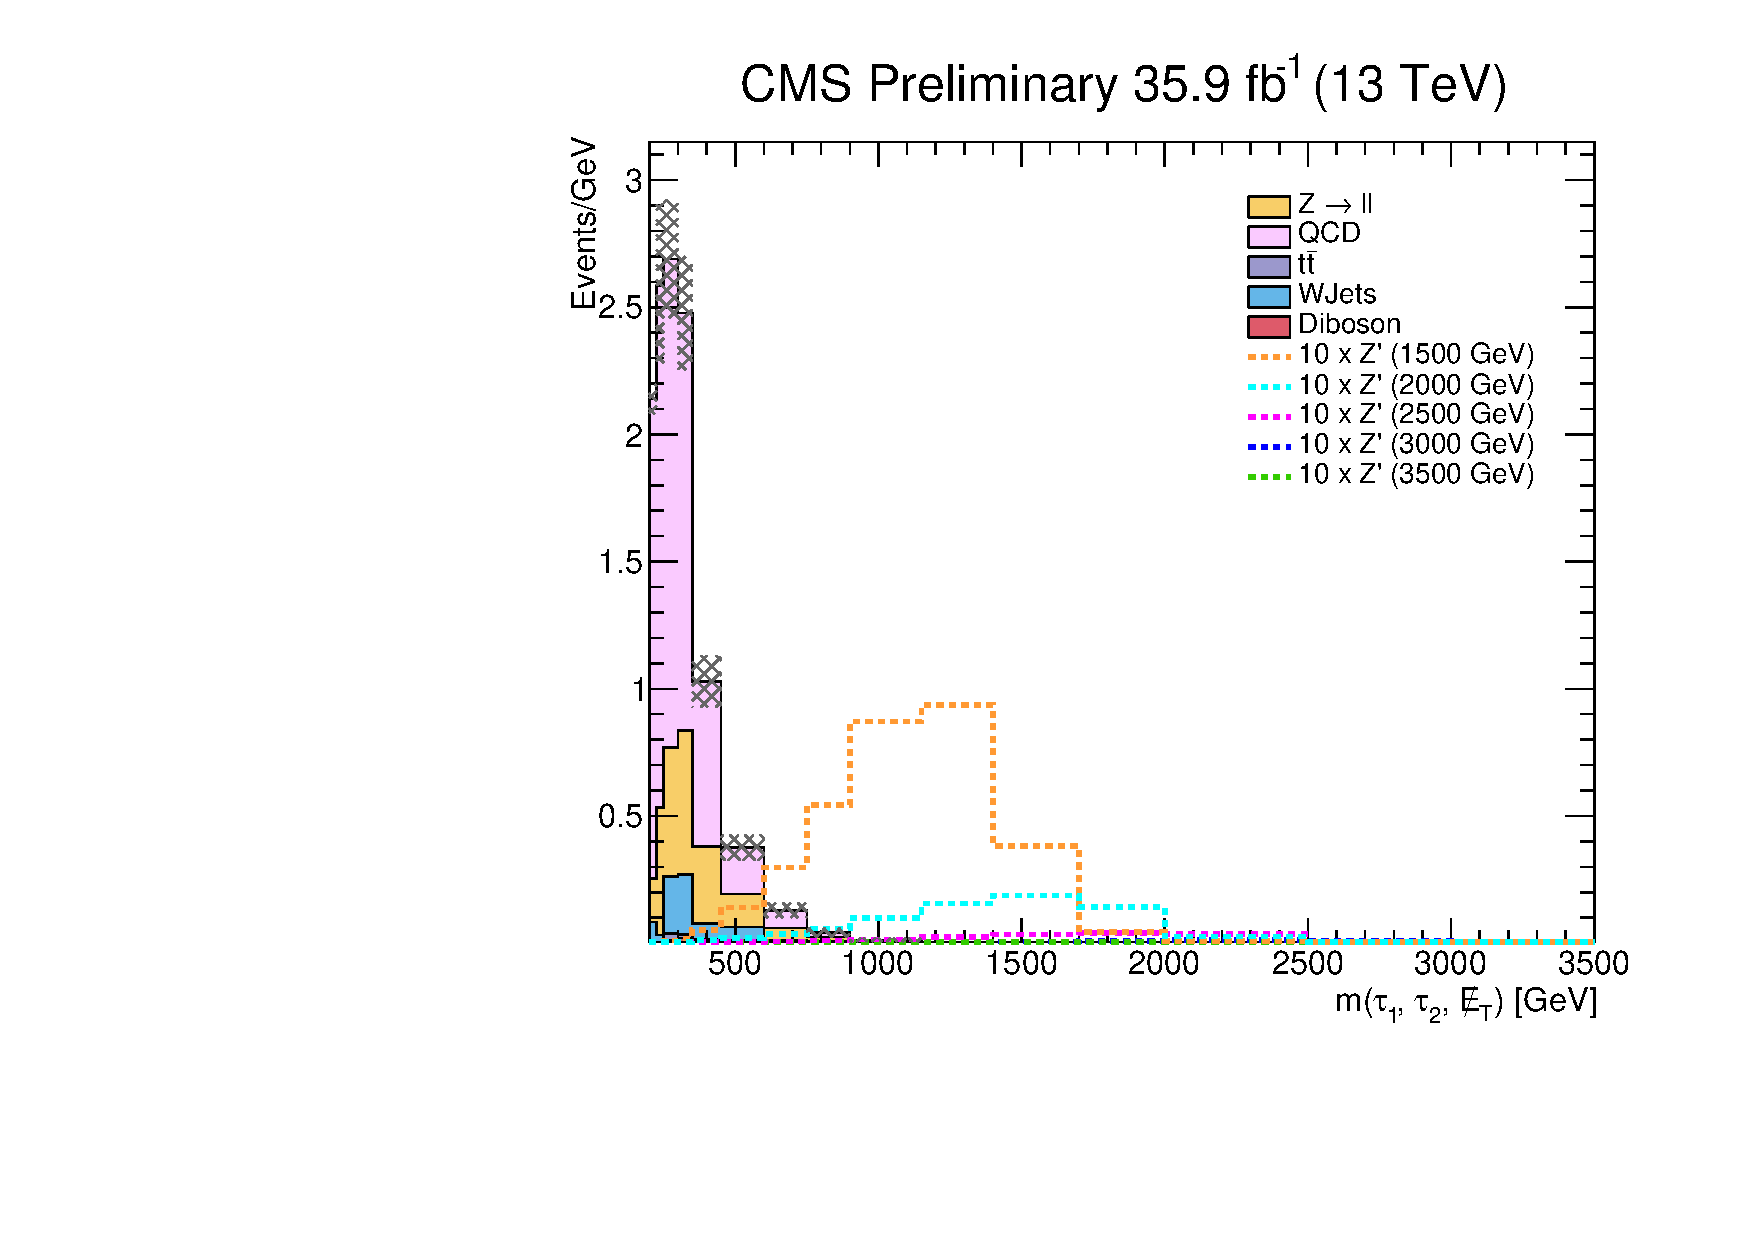
\includegraphics[clip,width=0.46\textwidth]{figuras/Chapter5/QCD_Estimation/Result_SR.pdf}
  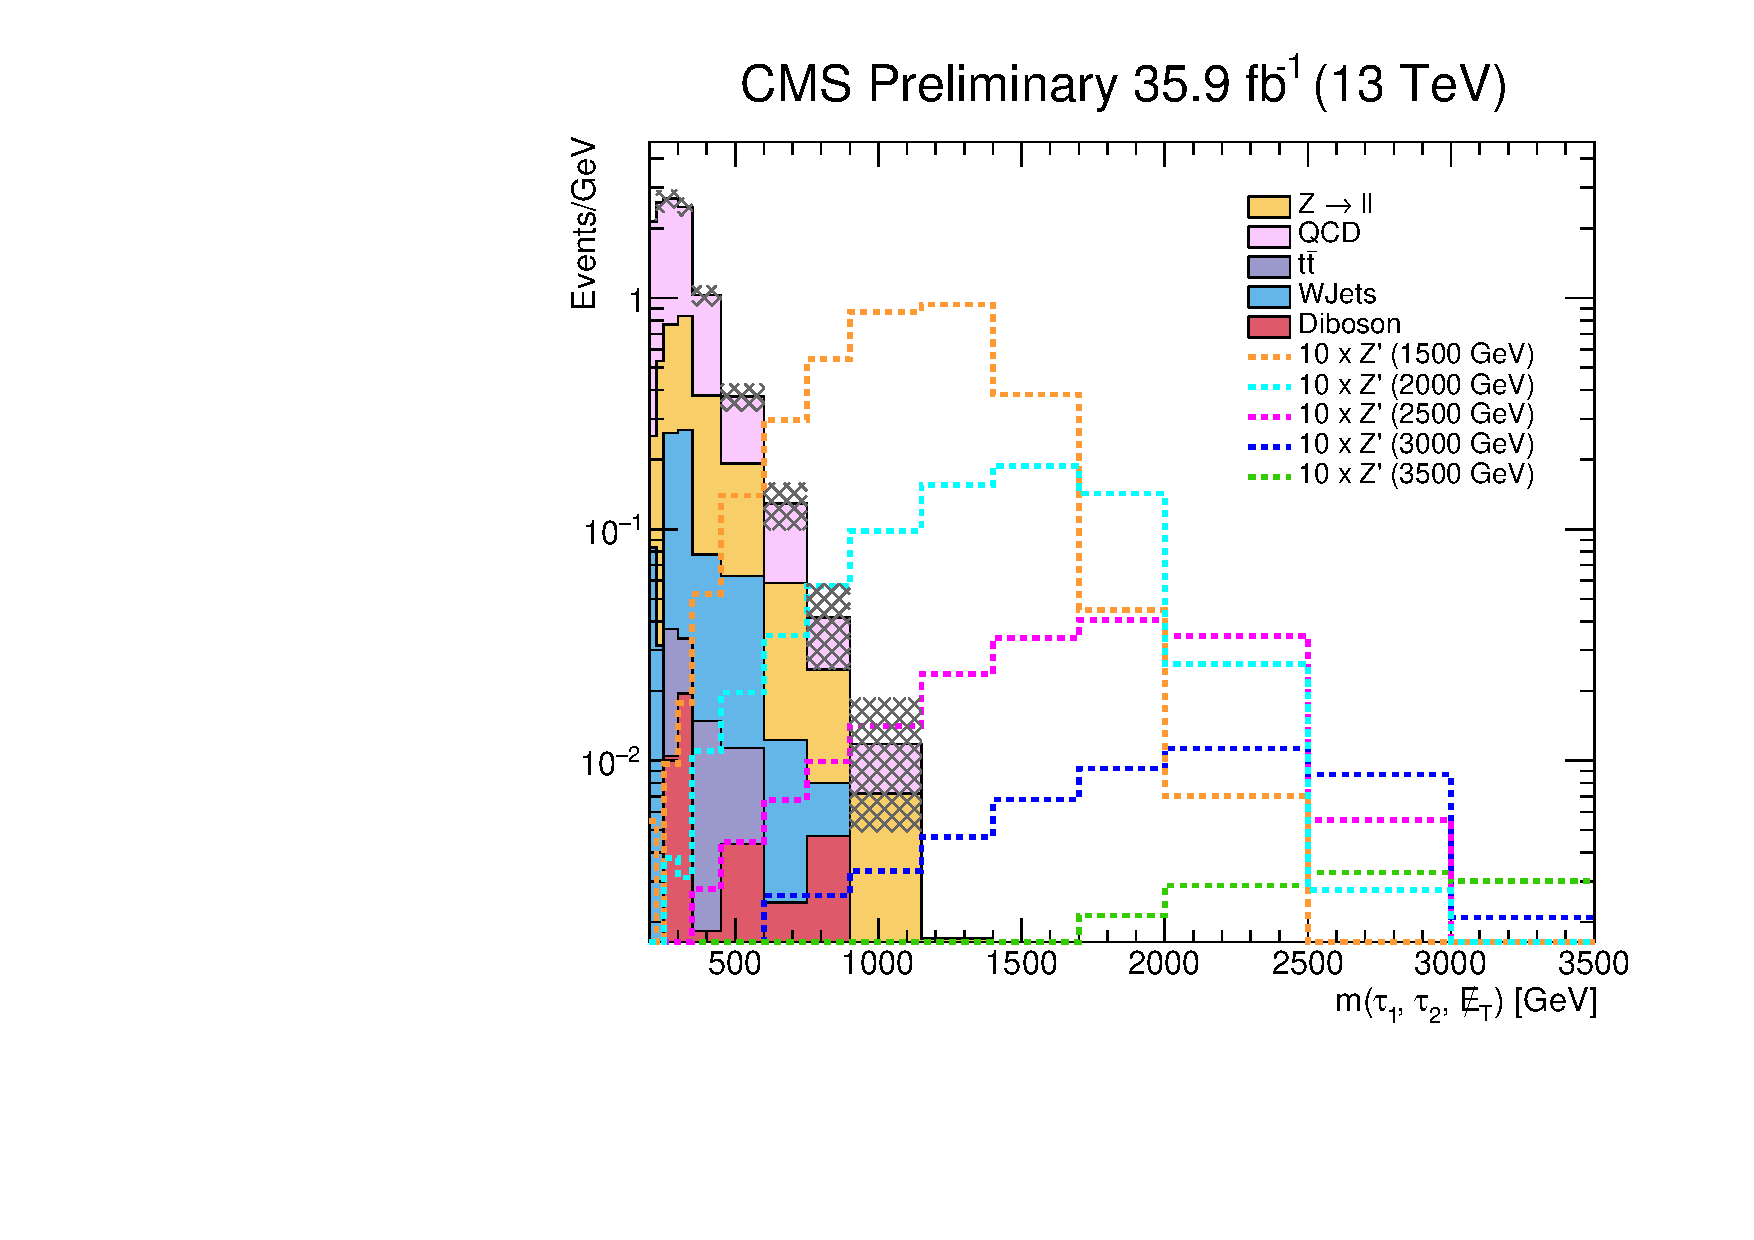
\includegraphics[clip,width=0.46\textwidth]{figuras/Chapter5/QCD_Estimation/Result_SR_log.pdf}
%   }
 \end{center}
 \caption{\mass~distribution in signal region using normal scale (left) and log scale (right). QCD 
 background was estimated from like-sign di-hadronic taus events in the 
 nominal-\MET~sideband, normalized with the $R_{OS/LS}$ ratio. Only the statistical uncertainties have been included.}
  \label{fig:SR_Result}	
 \end{figure}

\subsection{Background Estimation for Drell-Yan events}
\label{subsec:DY}

\noindent The Drell-Yan processes represent 23$\%$ of the total 
background and their estimation is performed 
using simulated samples. These samples are 
generally reliable since these kind of processes 
have been studied extensively. A control region 
dominated by this background is useful to 
validate the MC modeling as well as 
the tau identification used in this analysis. In such control 
region a good agreement between data and background is 
expected. However, the definition of an appropriate 
control region that allows to validate the simulated 
samples is not straightforward, considering 
that the di-hadronic tau final state is highly 
contaminated by QCD backgrounds, which must be 
estimated via data-driven methods. However,
a semi-clean sample with two high-quality 
hadronic taus can be obtained requiring a di-tau 
invariant mass less than 100 \GeV. Table \ref{tab:DYCR} shows 
the selection criteria used to define the  
enriched \Ztotauh~control sample.

\begin{table}[ht]
\begin{center}
\begin{tabular}{l|l} \hline \hline 
 \pt                          &  $>$  70 \GeV \\
 $|\eta|$                     &  $<$ 2.1 \\
 Tau Decay                     & \textit{1or3-prongs} \\
                              & \textit{newDMF} \\
 Isolation Disc.              & \textit{byTightIsolationMVArun2v1DBnewDMwLT} \\
 Anti-electron Disc.          & \textit{againstElectronMVALooseMVA6} \\
 Anti-muon Disc.              & \textit{againstMuonTight3} \\ \hline \hline 
 $\#$ b-jets (CSVv2 Loose WP) & $= 0$ \\
 $Ch_{\tau_{1}} \times Ch_{\tau_{2}} $ & $<$ 0 \\
 \DRt                         & $>$ 0.3  \\
 $m(\tau_{1},\tau_{1})$       & $<$ 100 \GeV \\ \hline \hline 
  \end{tabular}
  \end{center}
  \caption{Selection criteria used for the Drell-Yan control region.}
\label{tab:DYCR}
\end{table}

\begin{figure}[H]
 \begin{center}
 \captionsetup[subfloat]{farskip=0pt,captionskip=0.0cm,labelformat=empty}
 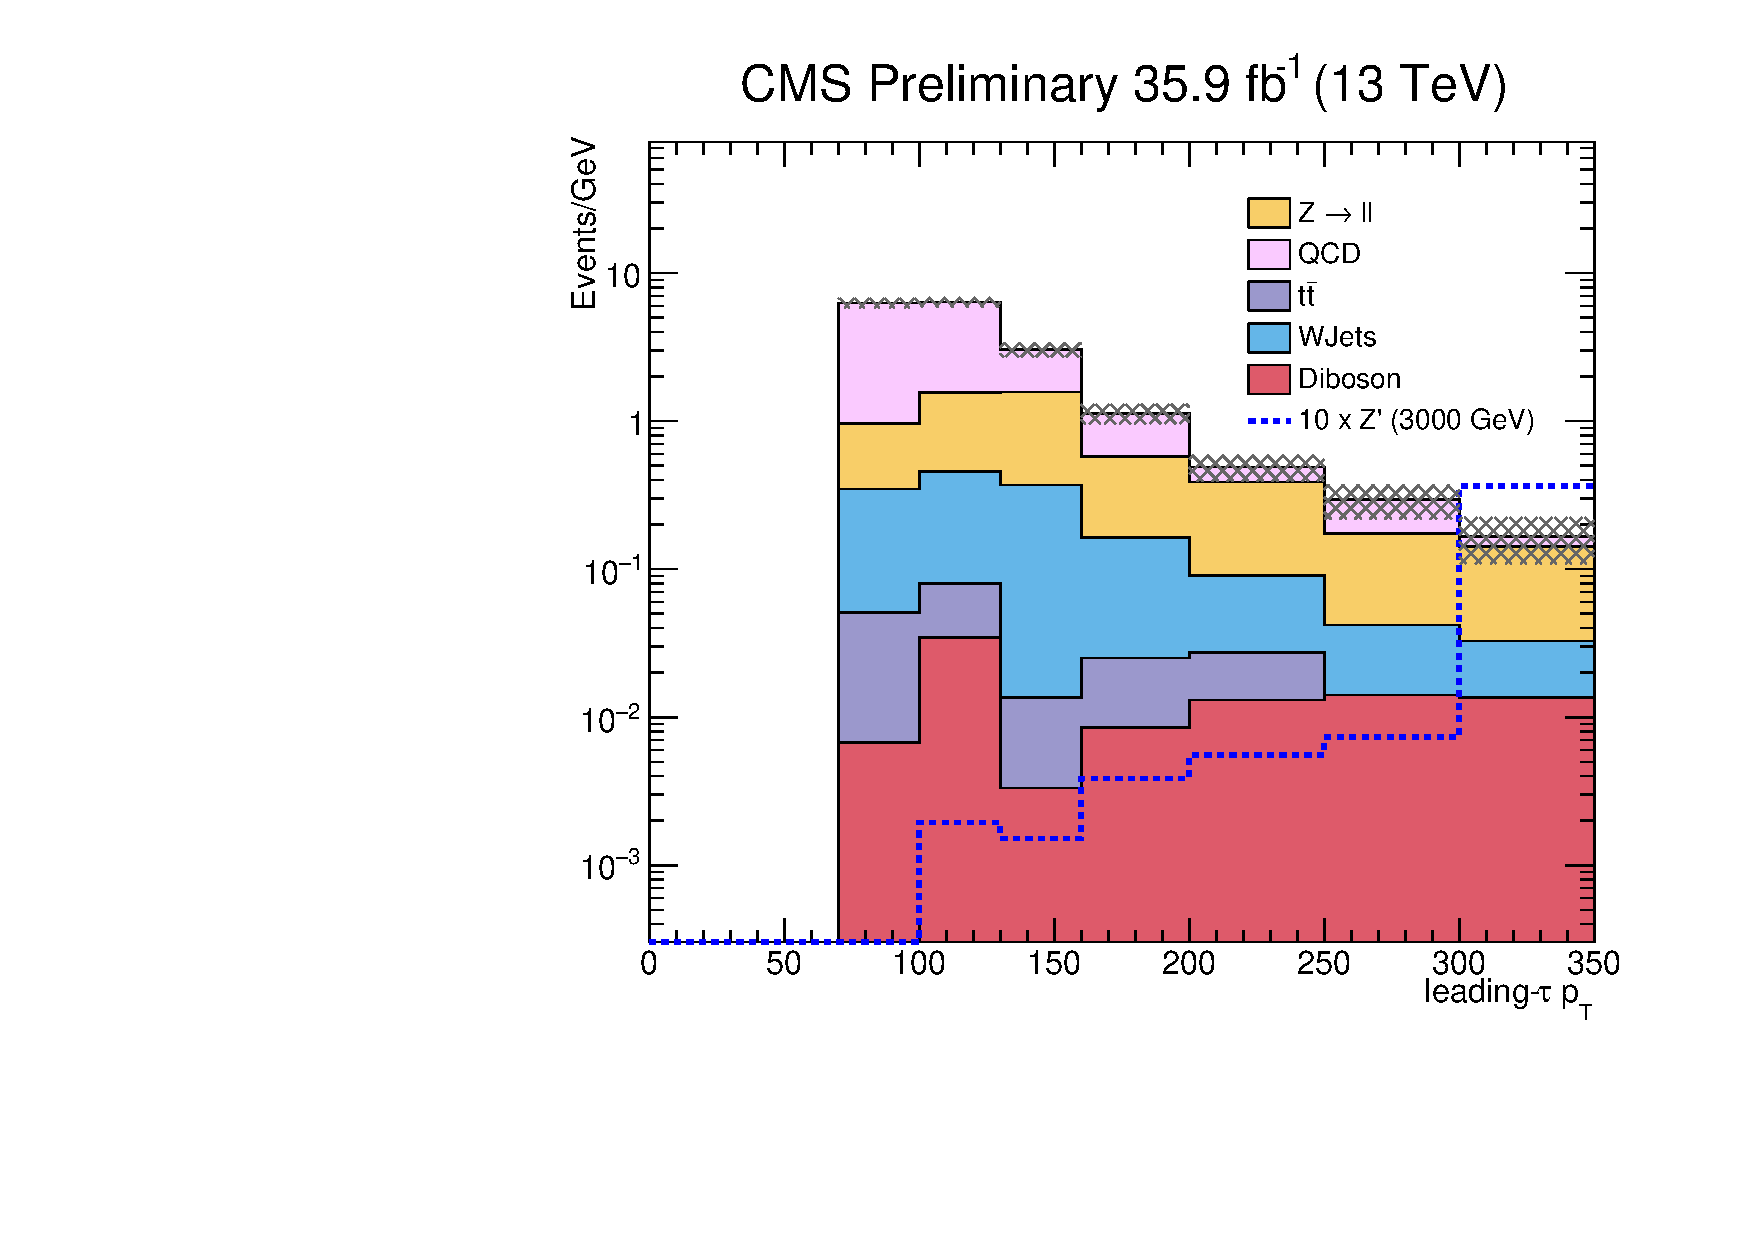
\includegraphics[clip,width=0.46\textwidth]{figuras/Chapter5/SR_Plots/leadtau_pt.pdf}
 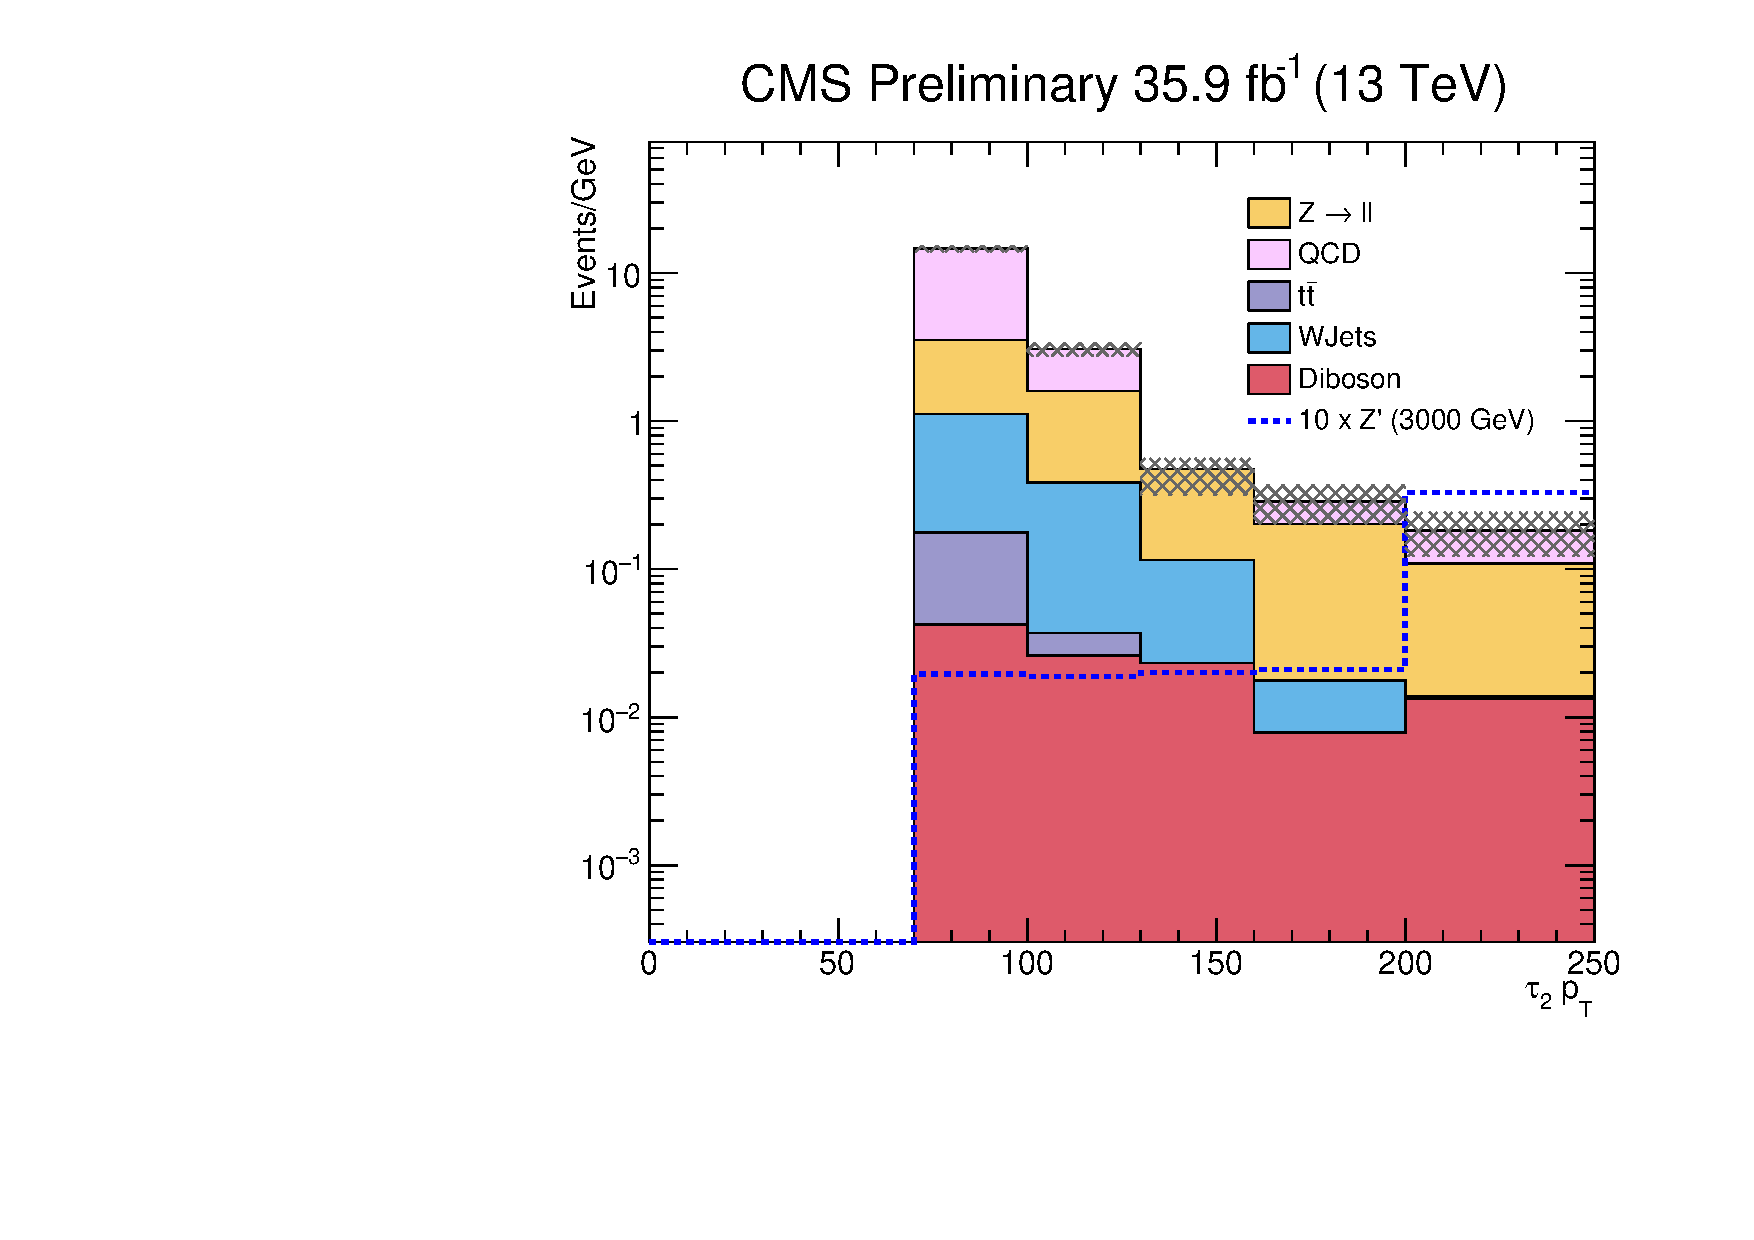
\includegraphics[clip,width=0.46\textwidth]{figuras/Chapter5/SR_Plots/tau2_pt.pdf} \hfill
 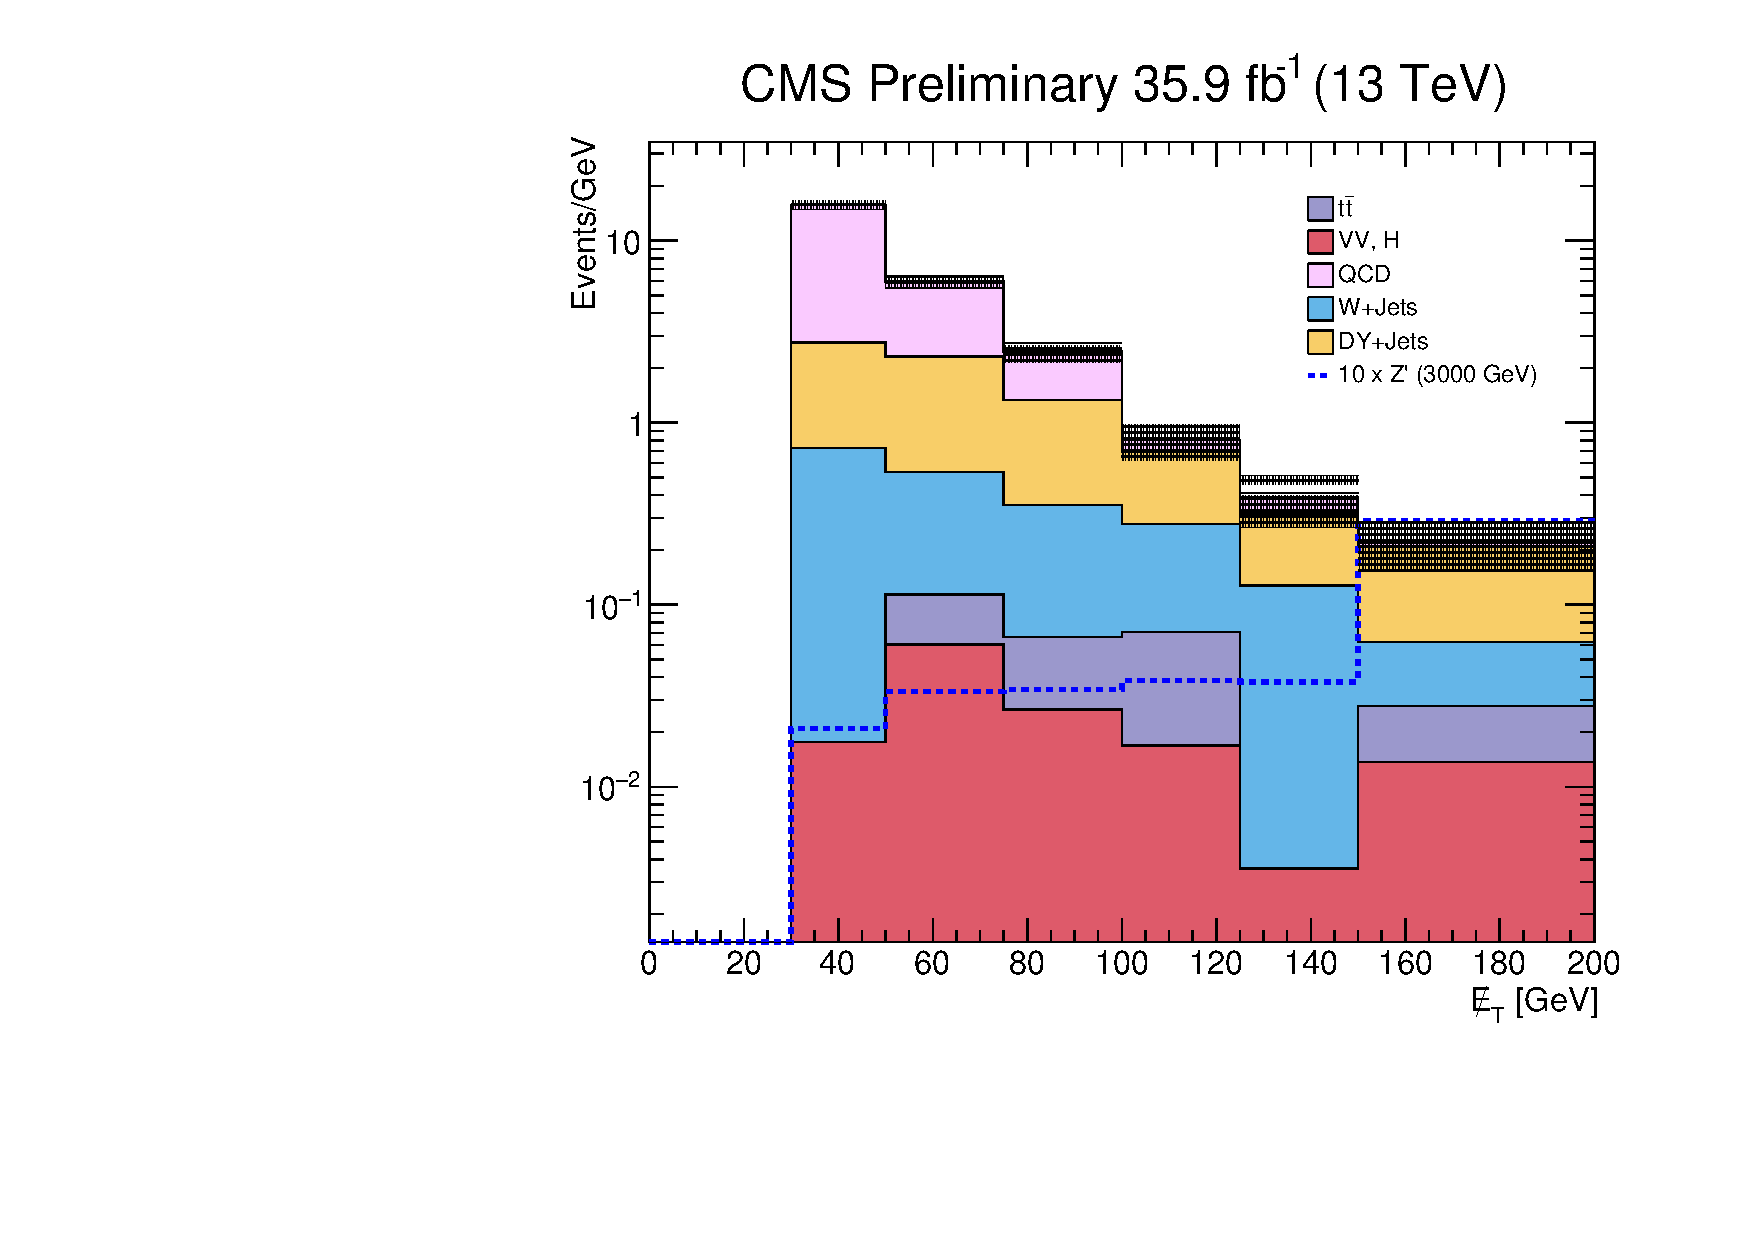
\includegraphics[clip,width=0.46\textwidth]{figuras/Chapter5/SR_Plots/MET.pdf}
 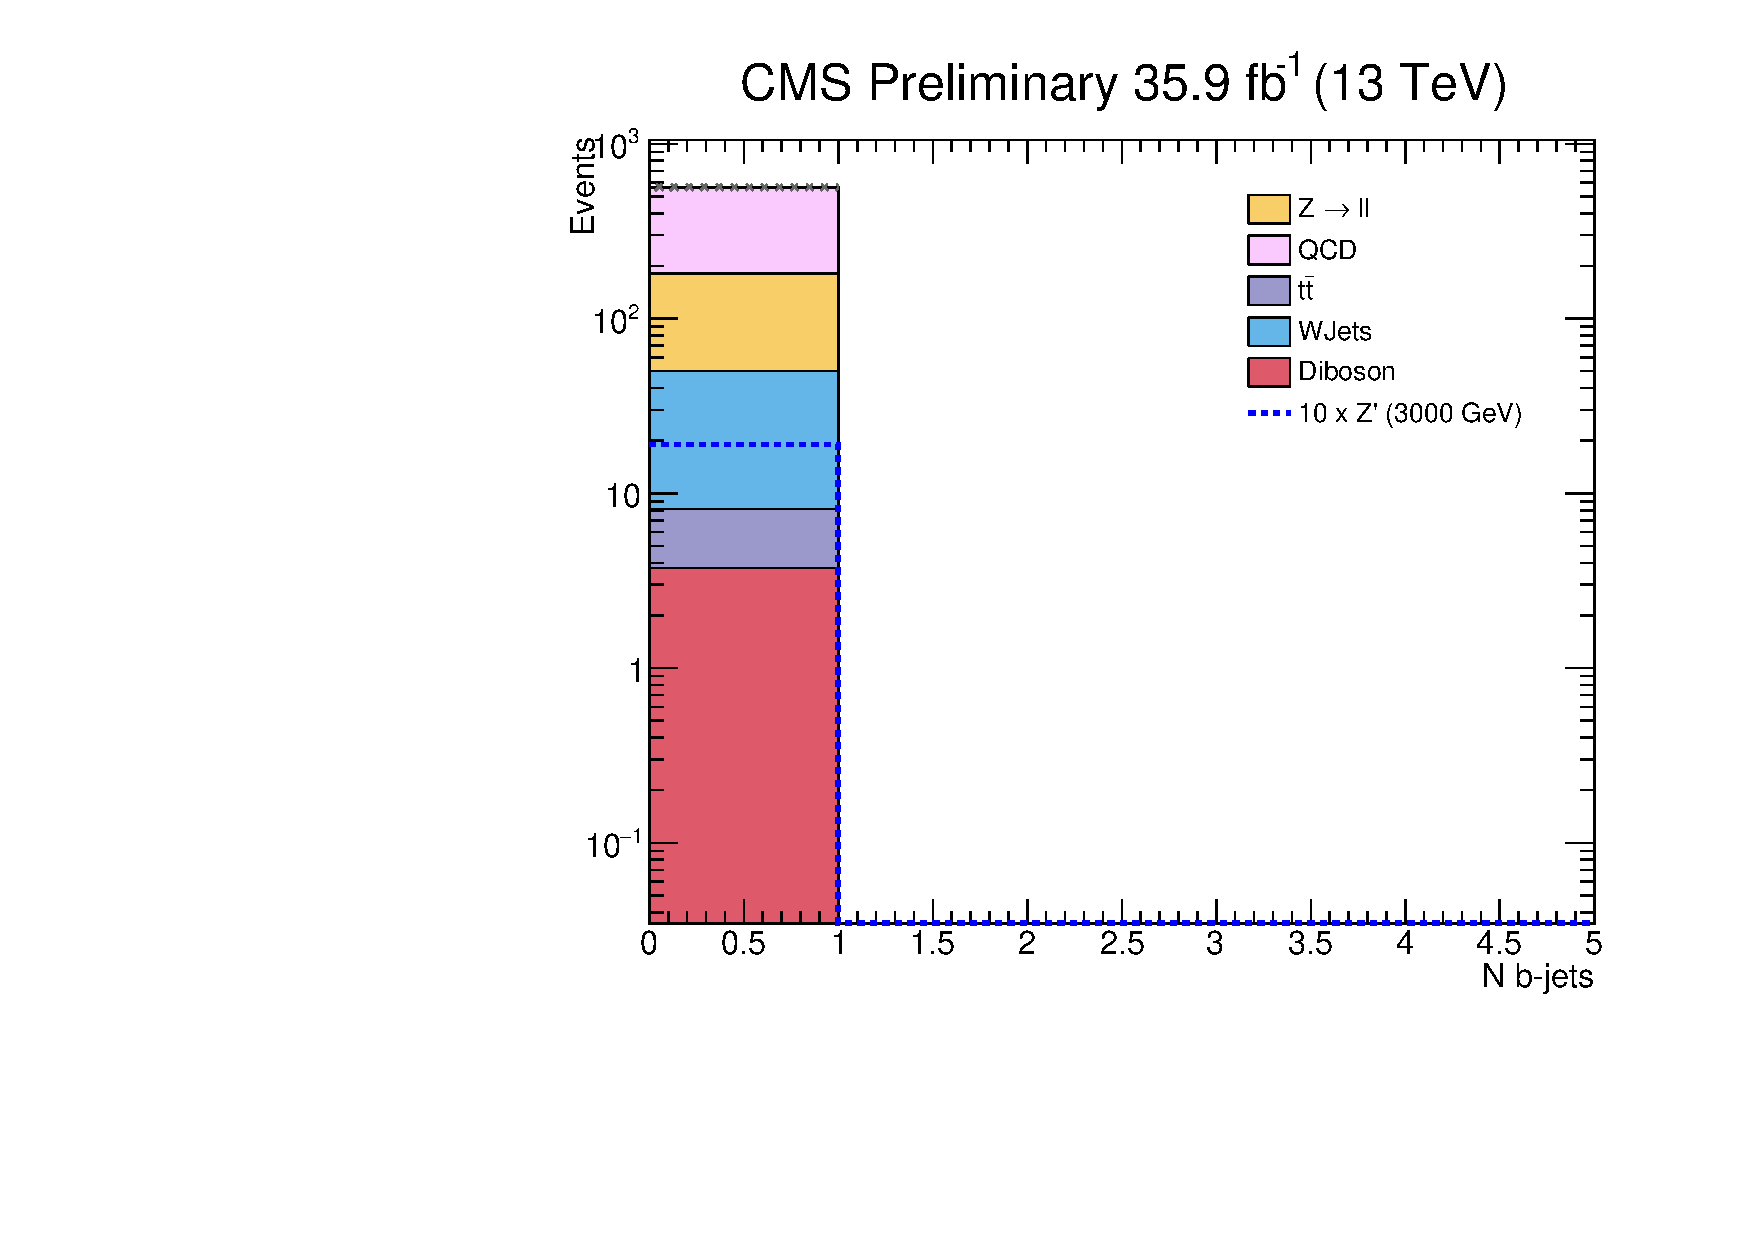
\includegraphics[clip,width=0.46\textwidth]{figuras/Chapter5/SR_Plots/NBJets.pdf}\hfill
 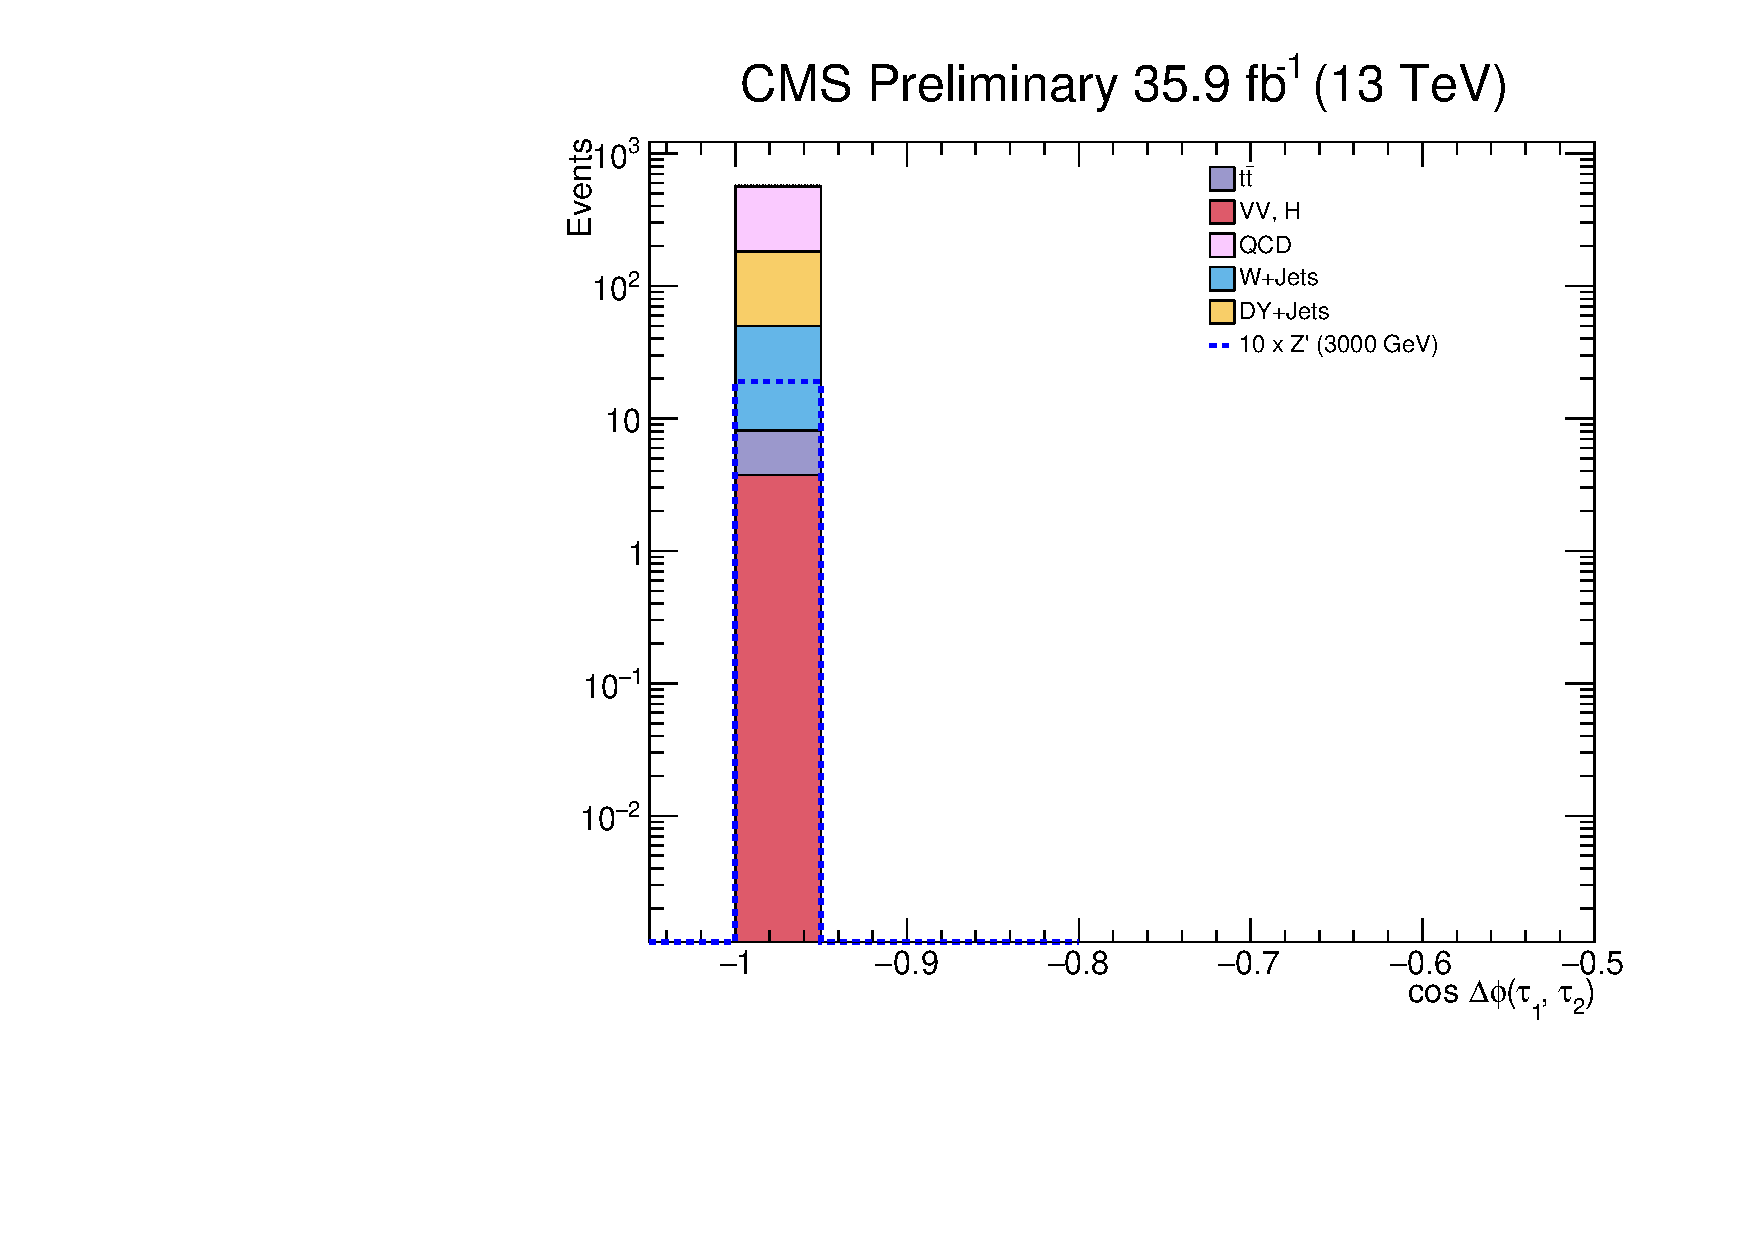
\includegraphics[clip,width=0.46\textwidth]{figuras/Chapter5/SR_Plots/cosDPhi.pdf}
 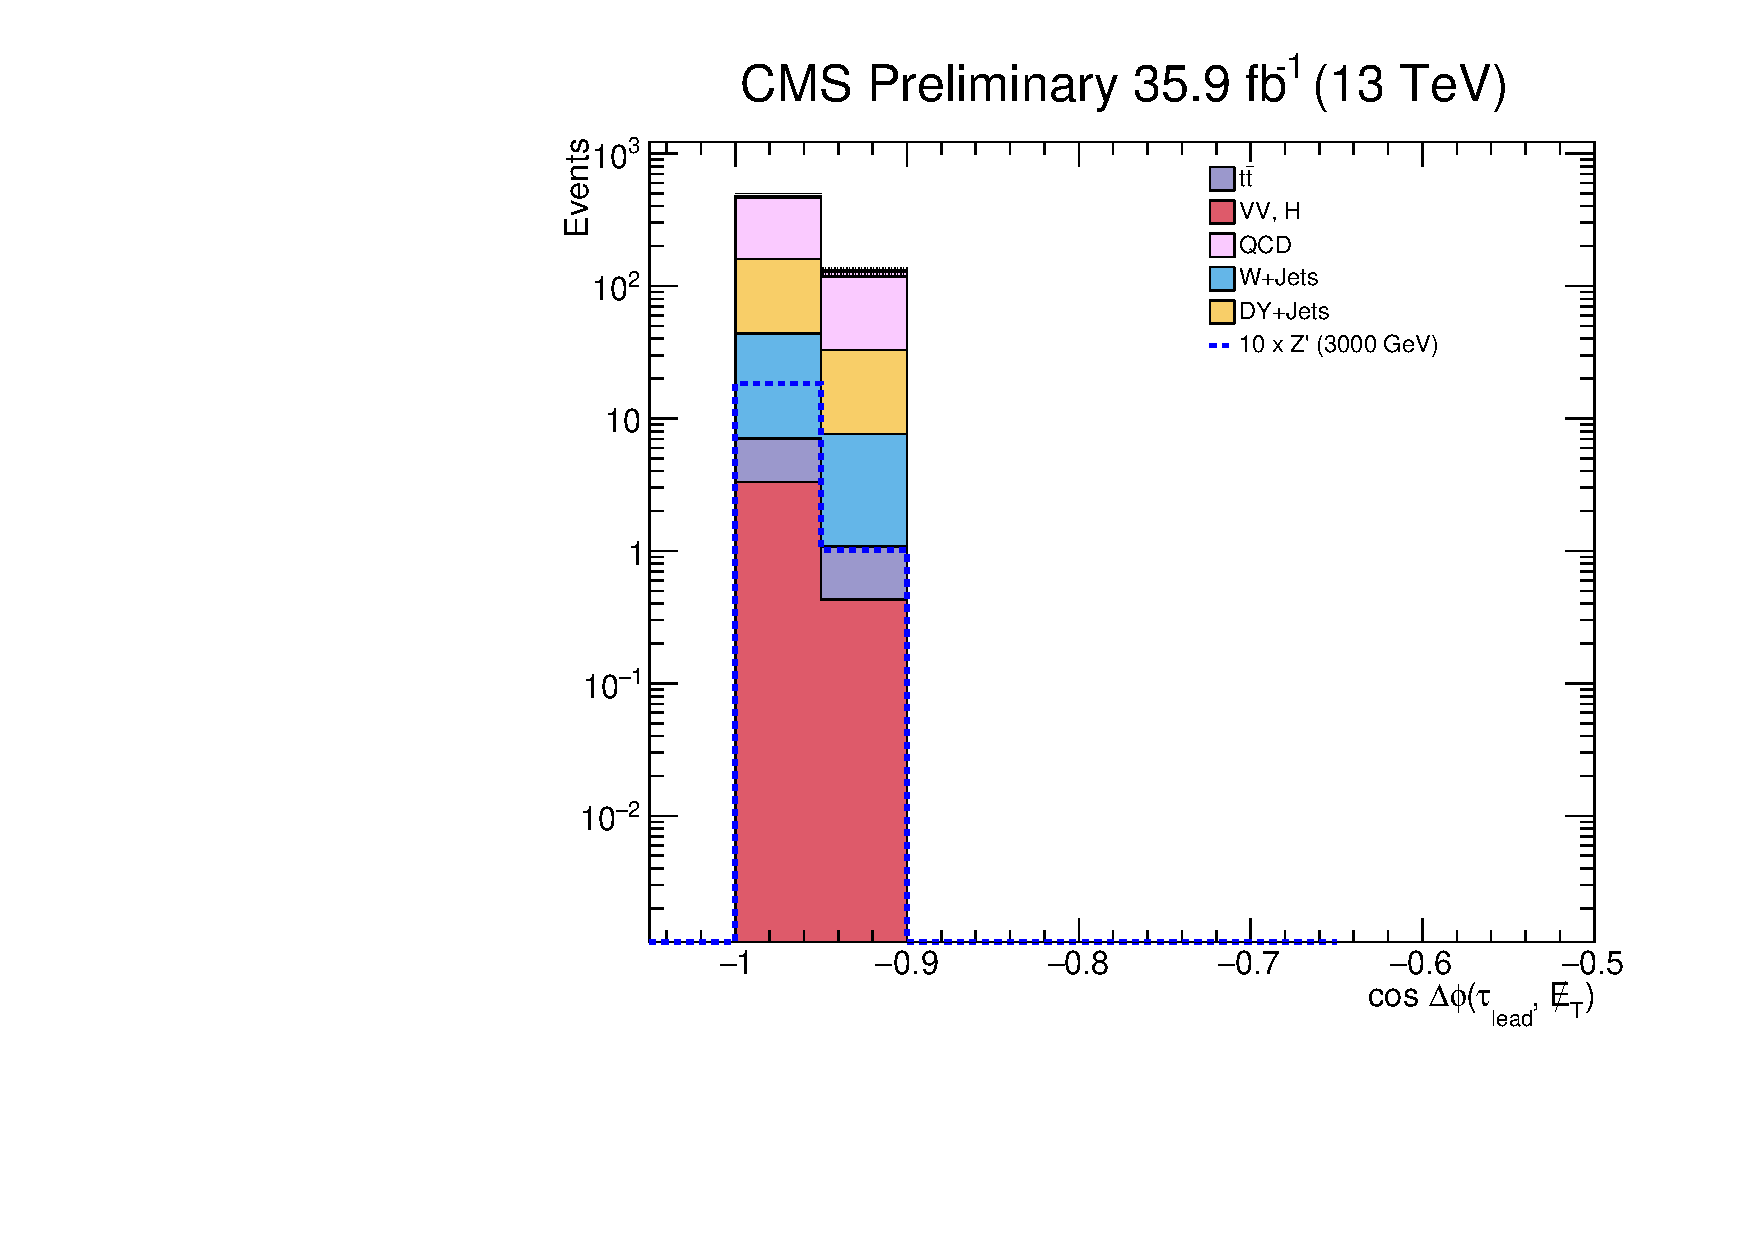
\includegraphics[clip,width=0.46\textwidth]{figuras/Chapter5/SR_Plots/cosTauMET.pdf} \hfill
 \end{center}
 \caption{Distribution of variables after all requirements for the signal region. The QCD 
 background was estimated from like-sign di-hadronic taus events in the 
 nominal-\MET~sideband, normalized with the $R_{OS/LS}$ ratio. The other backgrounds were estimated 
 directly from simulated samples. The uncertainty is only statistical. The variables plotted are:
 \pt~of the leading tau (top left),  \pt~of the second tau (top right), \MET~(middle left), number of b-jets (middle right), 
 $\cos\Delta \phi (\tau_{1},\tau_{2})$ (bottom left) and $\Delta \phi (\tau_{lead}, \not\!\!E_T)$ (bottom right).}
\label{fig:SignalRegionPlots}
 \end{figure}


\noindent Table \ref{tab:DYCRYields} shows the yields for the \Ztotauh~validation 
sample, where the QCD contribution has been determined using the method 
discussed in the previous section. Note that a good 
agreement between the data and the expected overall yield of 
the SM  is obtained since the $Data/MC$ ratio 
is 1.06 $\pm$ 0.09. Figure \ref{fig:DYCR} shows the di-hadronic tau 
invariant mass distribution, where the shape is consistent
with the SM prediction. In conclusion, since the $Data/MC$ ratio and 
the di-hadronic tau invariant mass shape are consistent with 
the SM expectation, the Drell-Yan processes, as well as the tau identification, 
are well modeled by the simulated samples.

\begin{table}[ht]  
\begin{center}
\begin{tabular}{ | l | r |} \hline \hline 
 \multicolumn{2}{|c|}{DY CR Yields} \\ \hline \hline 
 \textbf{Data}         & \textbf{431.00}  $\pm$  \textbf{ 20.76} \\ \hline 
 DY           & 346.24   $\pm$   25.09 \\ \hline 
 WJets      & 3.27   $\pm$   1.02 \\ \hline 
 DiBoson    & 17.43   $\pm$   1.39 \\ \hline 
 \ttbar     & 1.70   $\pm$   0.77 \\ \hline 
 QCD        & 37.90   $\pm$   8.45 \\ \hline 
 \textbf{TOTAL BKG} & \textbf{ 406.54}   $\pm$  \textbf{ 26.54} \\ \hline 
 \textcolor{blue}{Data/MC}         & \textcolor{blue}{1.06}  $\pm$  \textcolor{blue}{ 0.09} \\ \hline 
 \end{tabular}  
\end{center}
  \caption{Background and data yields in \Ztotauh~region obtained using the DY selection criteria.}
\label{tab:DYCRYields}
\end{table}

\begin{figure}[H]
\begin{center}
\captionsetup[subfloat]{farskip=0pt,captionskip=0.0cm,labelformat=empty}
\resizebox{\textwidth}{8.8cm}{
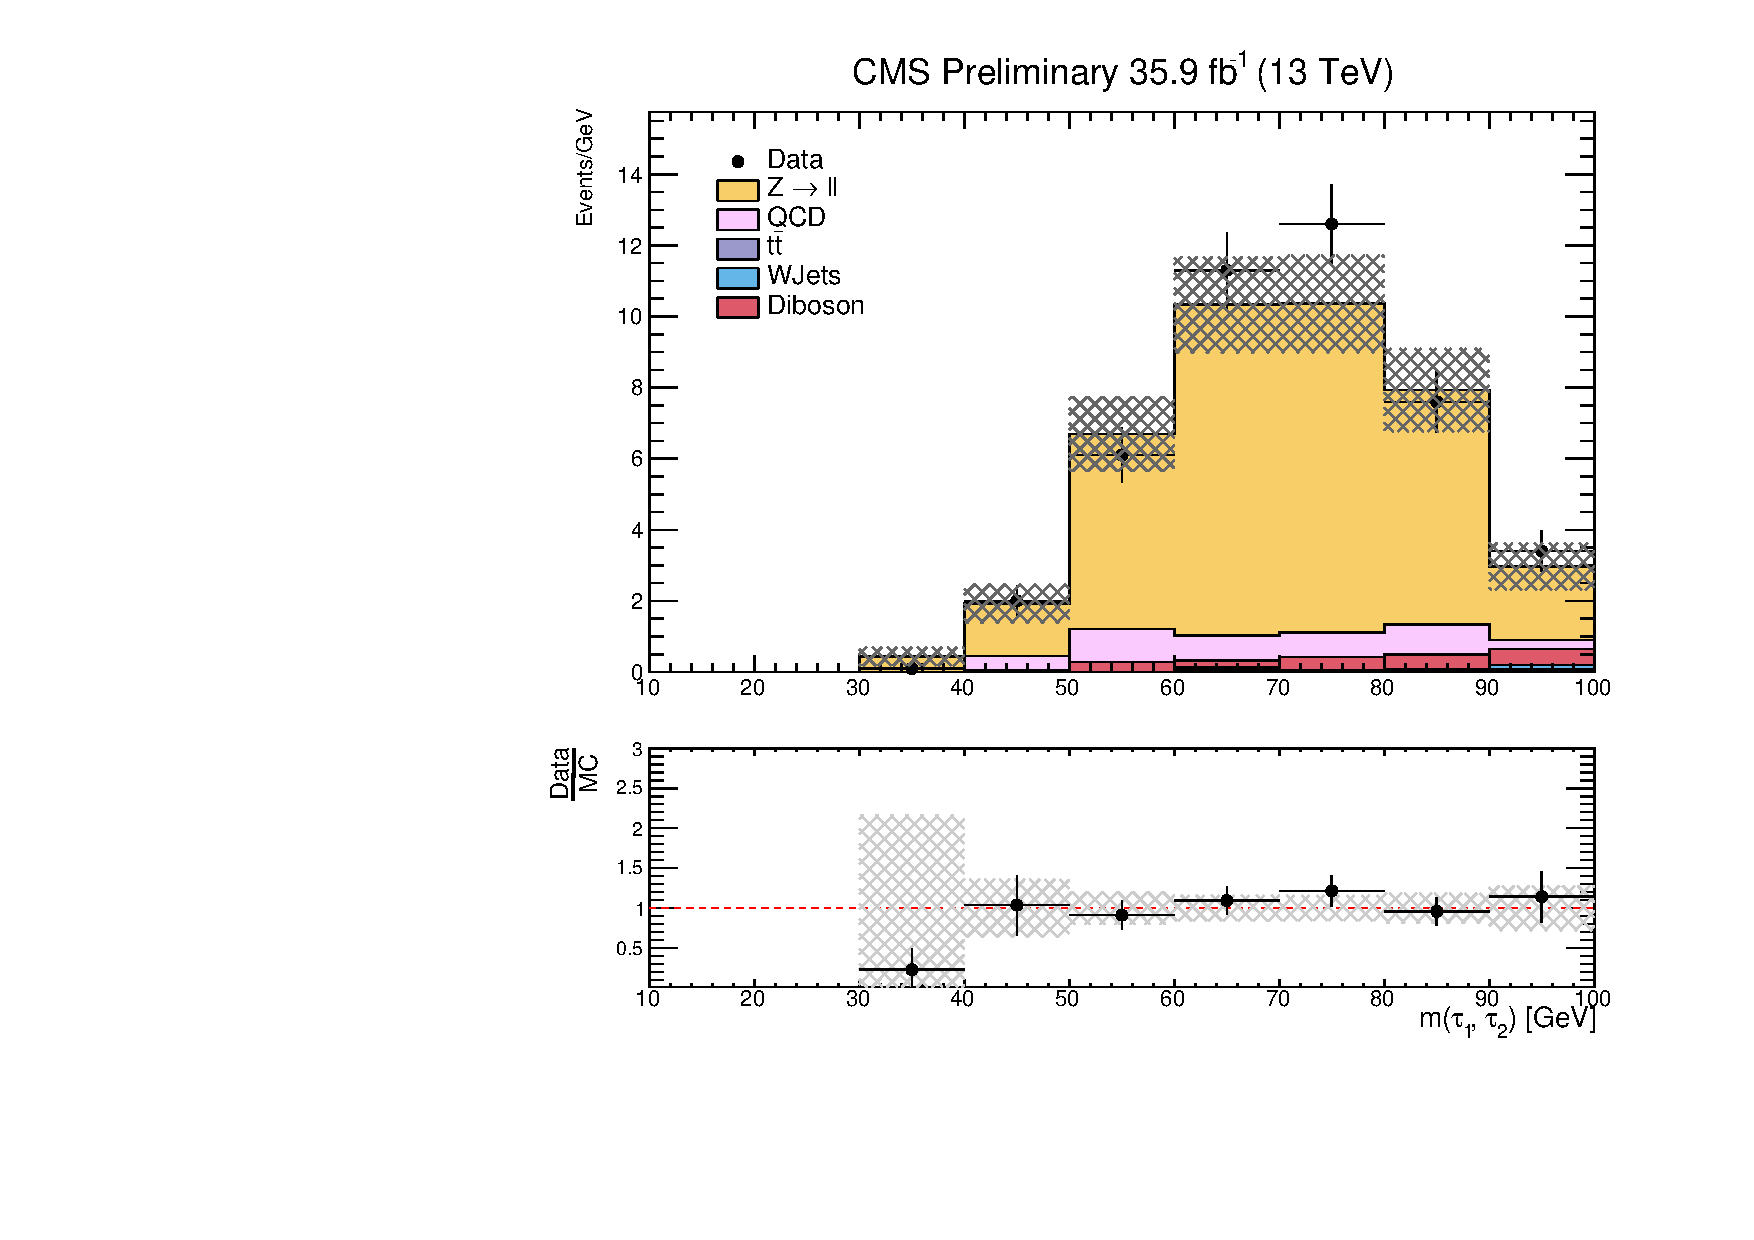
\includegraphics[clip,width=0.46\textwidth]{figuras/Chapter5/DY_Estimation/DY_CR_mio.pdf}
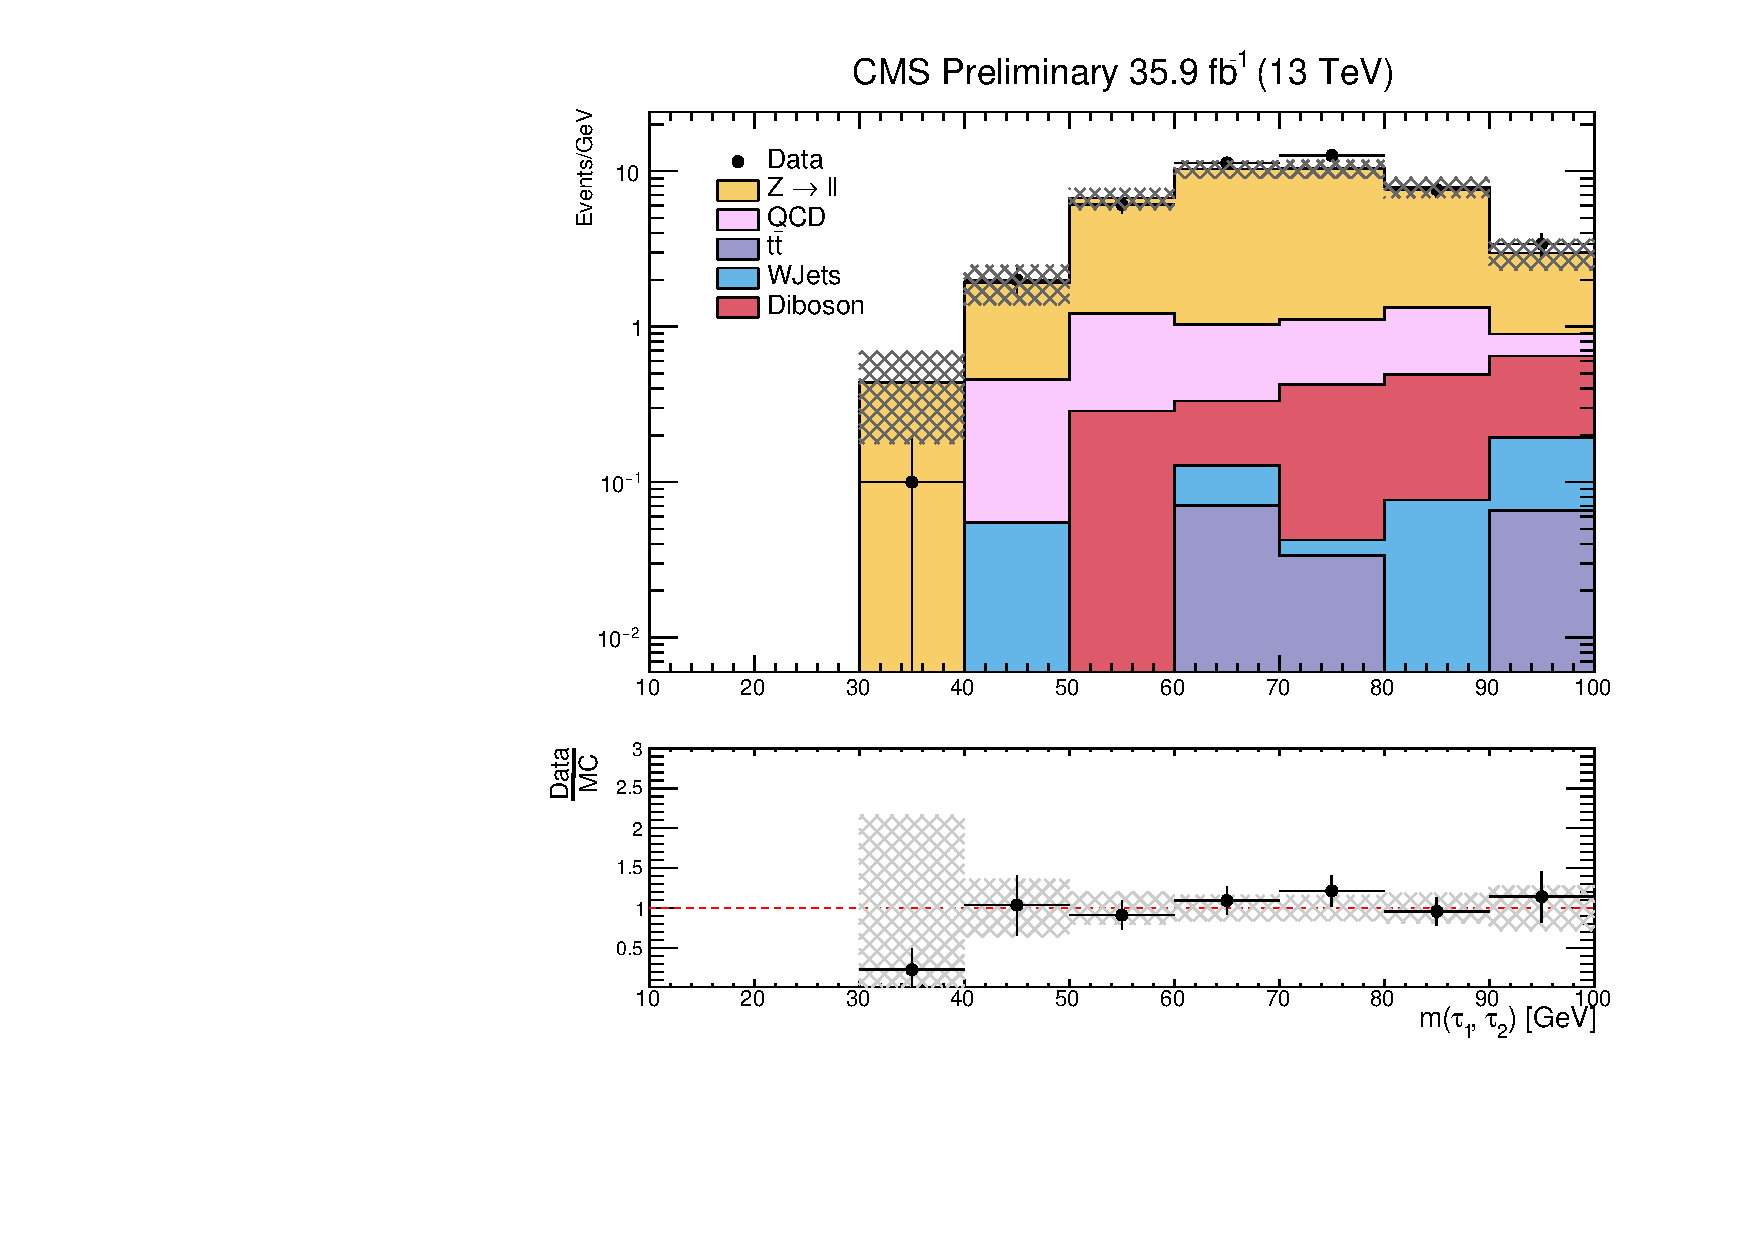
\includegraphics[clip,width=0.46\textwidth]{figuras/Chapter5/DY_Estimation/DY_CR_log_mio.pdf}
}
\end{center}
\caption{$m(\tau_{h},\tau_{h})$ distribution for the region obtained using the 
DY selection criteria. Linear scale (left), log scale (right). Only the statistical uncertainties have been included.}
\label{fig:DYCR}
\end{figure}


\subsection{Validation}
\label{subsec:Validation}

\noindent Besides the (N-1) distributions shown in Figure \ref{nminusone},
other way to validate the background estimation is inverting the 
$\cos \Delta \phi (\tau_{1},\tau_{2})$ cut; since in such region 
the signal contamination is minimum and there is still enough statistics 
for background estimation. Then, the validation 
region is defined by:

\begin{itemize}
 \item -0.95 $<$ $\cos\Delta \phi (\tau_{1},\tau_{2}) <$ 1.0
 \item \MET~$>$ 30 \GeV
 \item $\Delta \phi (\tau_{lead}, \not\!\!E_T) <$ -0.9
 \item no jets with \pt~greater than 30 \GeV~tagged as b-jets
\end{itemize}

\noindent Figure \ref{fig:cosDphiInv} shows distributions of variables after applying
the selection criteria listed above. The agreement between the data and the simulated
samples confirms the proper estimation of the background; any disagreement
between them is due to the low statistics.

\section{Corrections for Simulated Events}
\label{sec:PUCorrection}

\noindent Although the event simulations developed by the particle physics
community have been extensively studied and upgraded for years, there are still
differences between the simulated events of SM processes and the observed 
data. Therefore, corrections must be applied on the simulated events
in order to minimize such differences and, consequently, in order
to improve the accuracy of expected yield, for both, backgrounds and 
signal simulated samples. The corrections applied are 
described in this section.\\

\textbf{Pile-Up corrections} \\

\noindent The official simulated samples, certified by the CMS collaboration, usually 
are produced at the same time, or before, the data-taking period. Considering 
that the pileup interactions depend on the LHC operational conditions, the simulated 
samples are generated including the effect of the expected 
pileup interactions during the data-taking period; however, exactly 
the LHC operational parameters are not necessarily the same 
used for the event generation. As a result, the MC samples 
have different pileup distributions than those of real 
data. In consequence, the simulated events must be 
weighted properly in order to reproduce the pileup distribution
observed in data. \\

\noindent The method employed by the CMS collaboration in order to measure 
the number of pileup interactions in the data consists on multiplying 
the instantaneous luminosity, for a single bunch crossing,
by the total inelastic cross section. This method is reliable
since the instantaneous luminosity for a single BX can be computed
from the LHC operational parameters, and the total inelastic 
cross-section, that has been measured. As a result, a certified JSON file 
is issued, containing the pileup information for the 
entire data-taking period. Thus, the probability to 
obtain $n$ interactions in a data event ($P_{data}(n)$) can be estimated. \\
% such as the revolution frequency, 

\noindent The pileup weight applied on a simulated event is given by:

\begin{equation}
w(n) = \frac{P_{data}(n)}{P_{MC}(n)}
\end{equation}

\begin{figure}[H]
 \begin{center}
 \captionsetup[subfloat]{farskip=0pt,captionskip=0.0cm,labelformat=empty}
 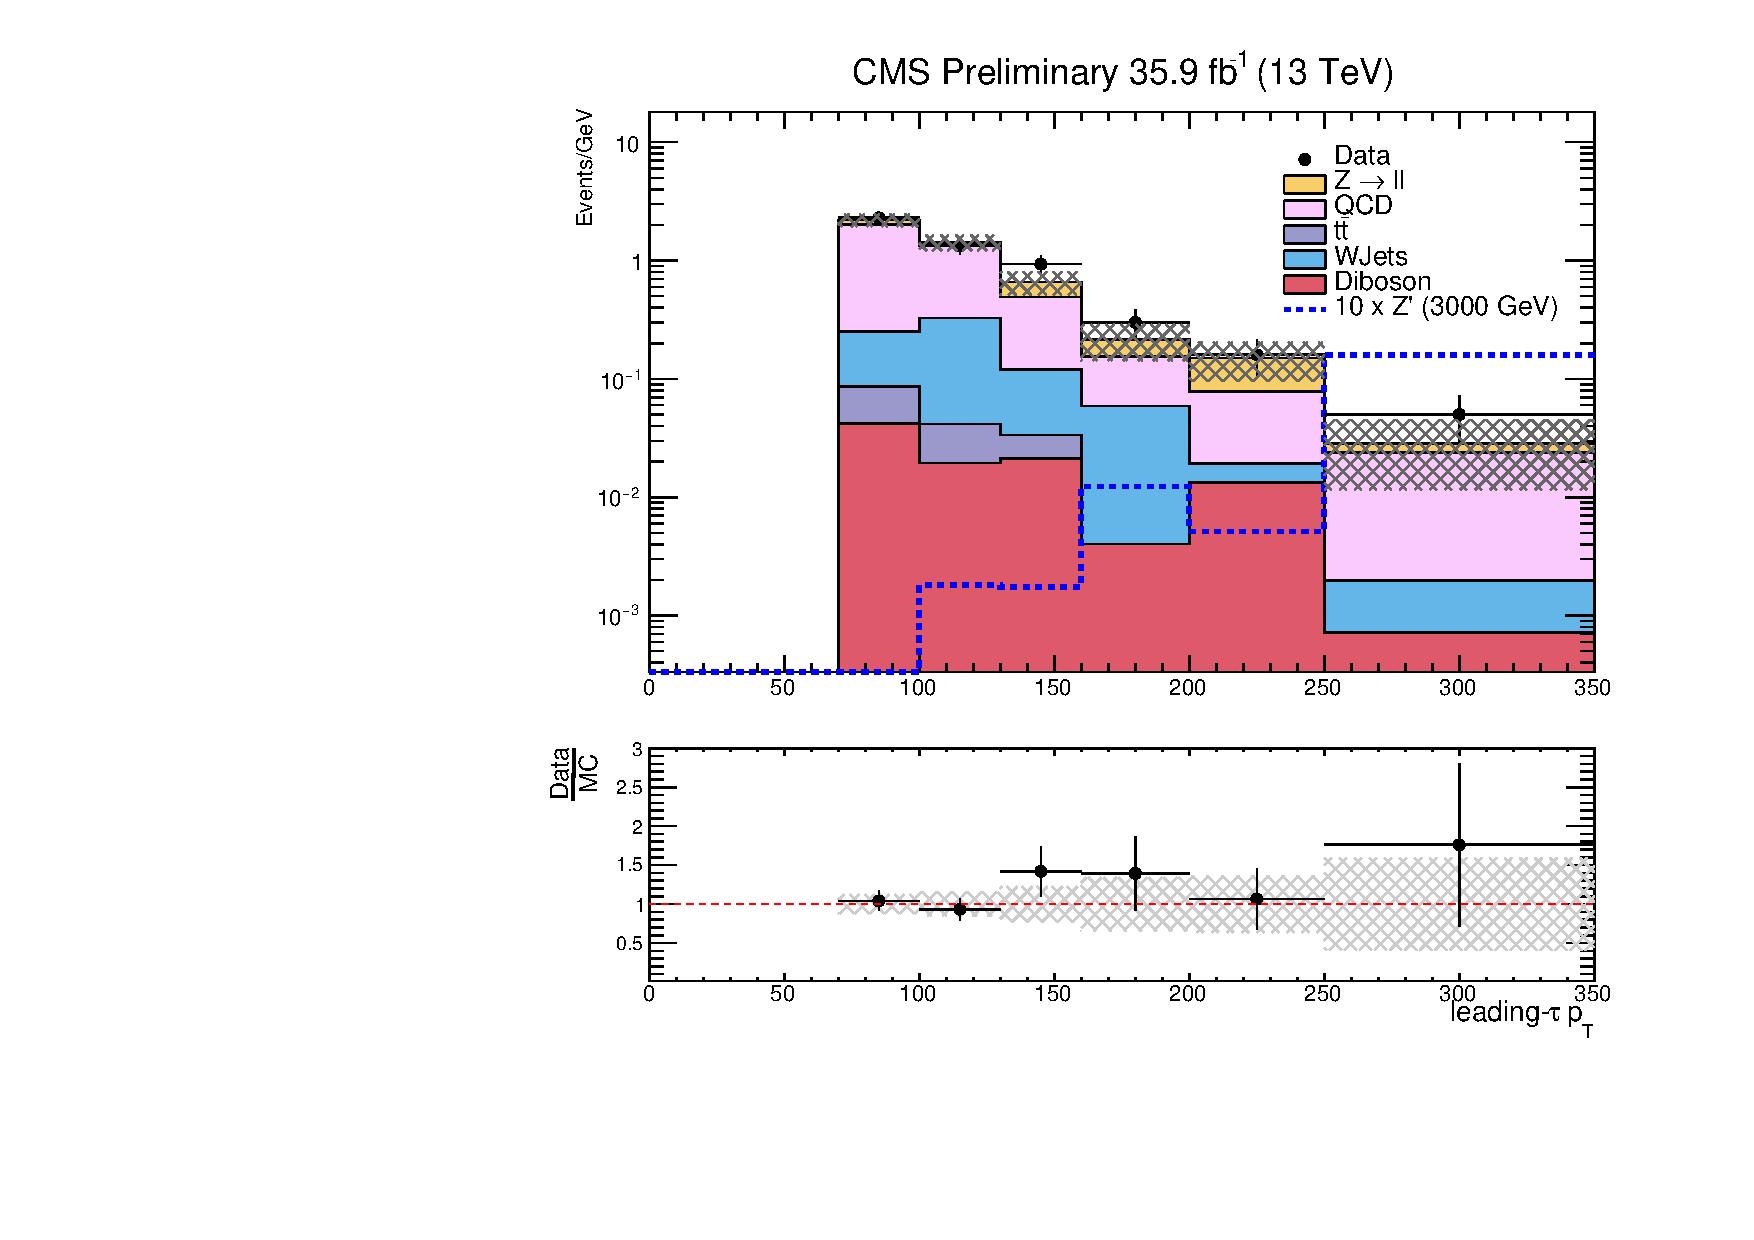
\includegraphics[clip,width=0.46\textwidth]{figuras/Chapter5/Plots_CosDphiInv/leadtaupt.pdf}
 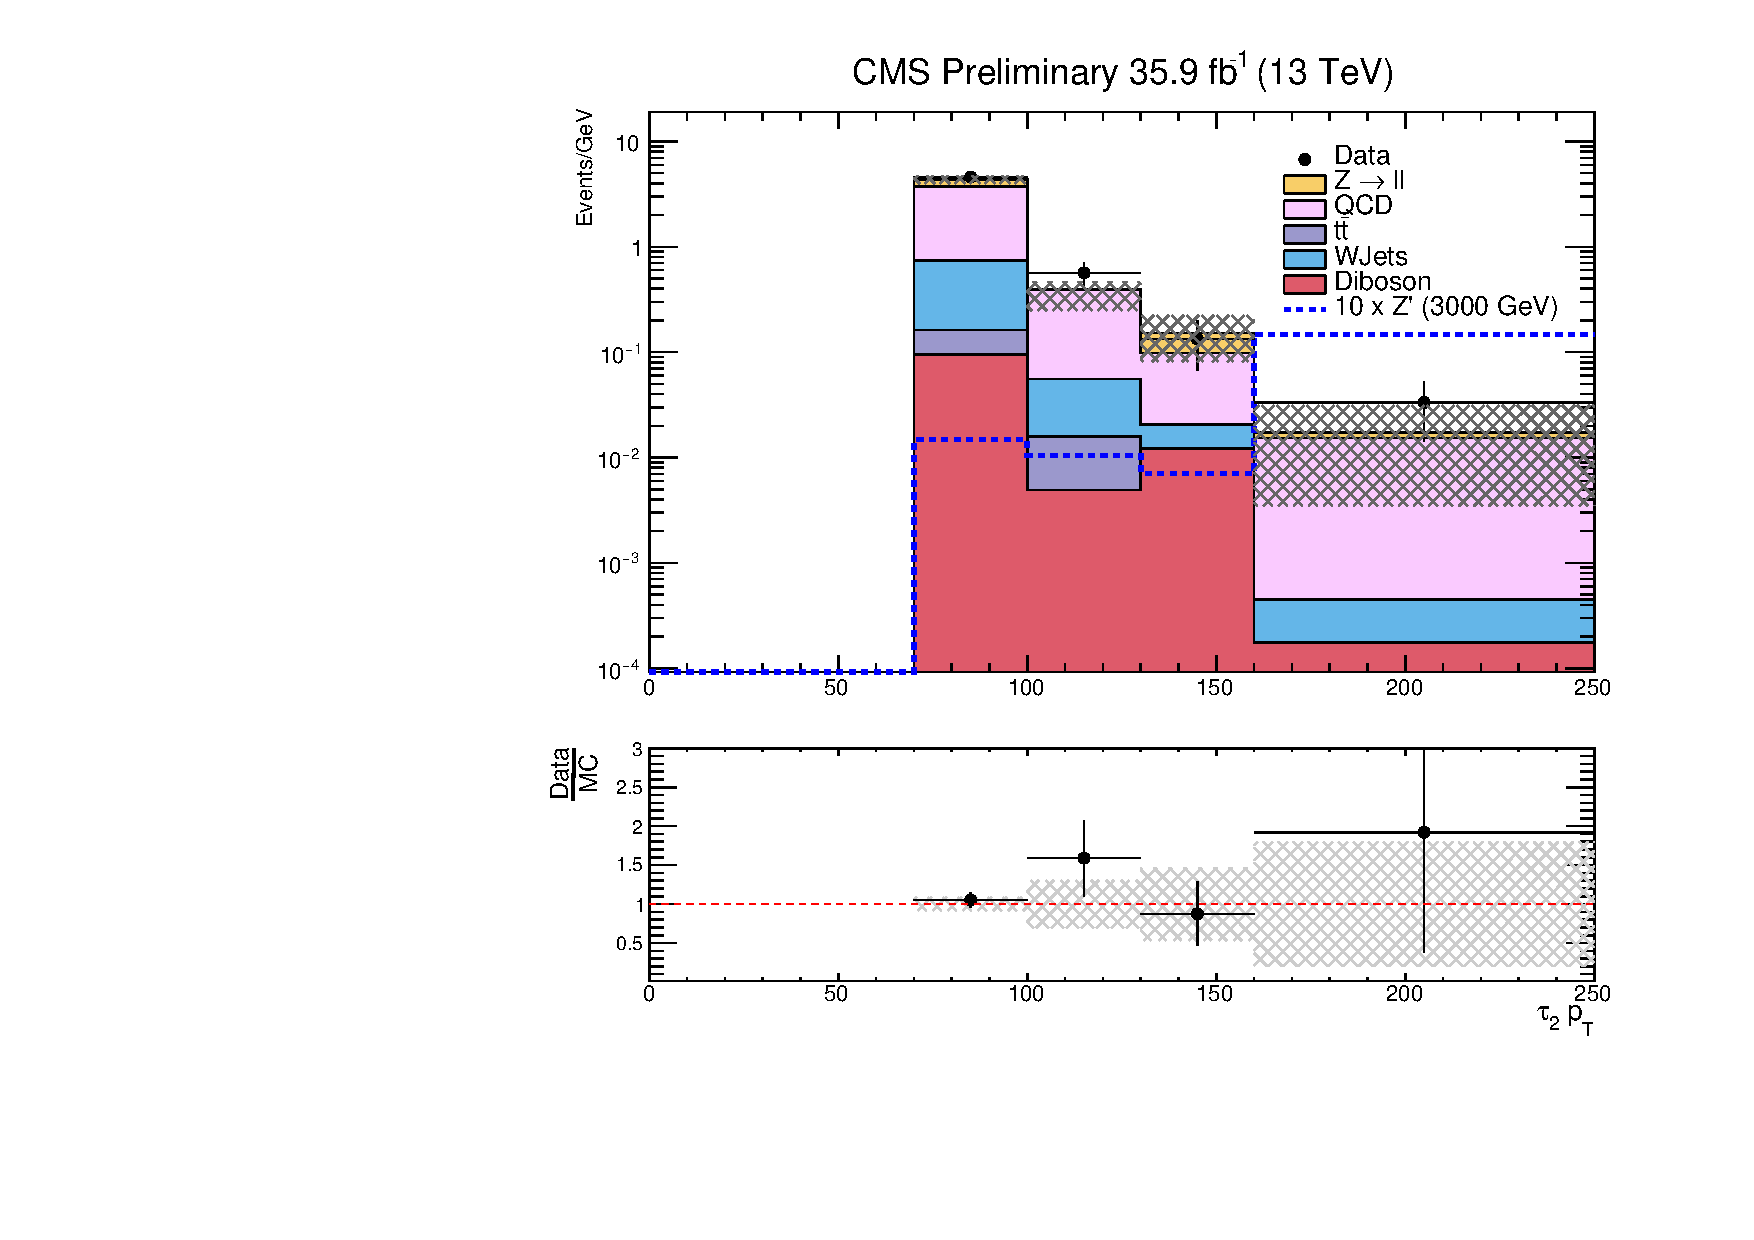
\includegraphics[clip,width=0.46\textwidth]{figuras/Chapter5/Plots_CosDphiInv/tau2pt.pdf} \hfill
 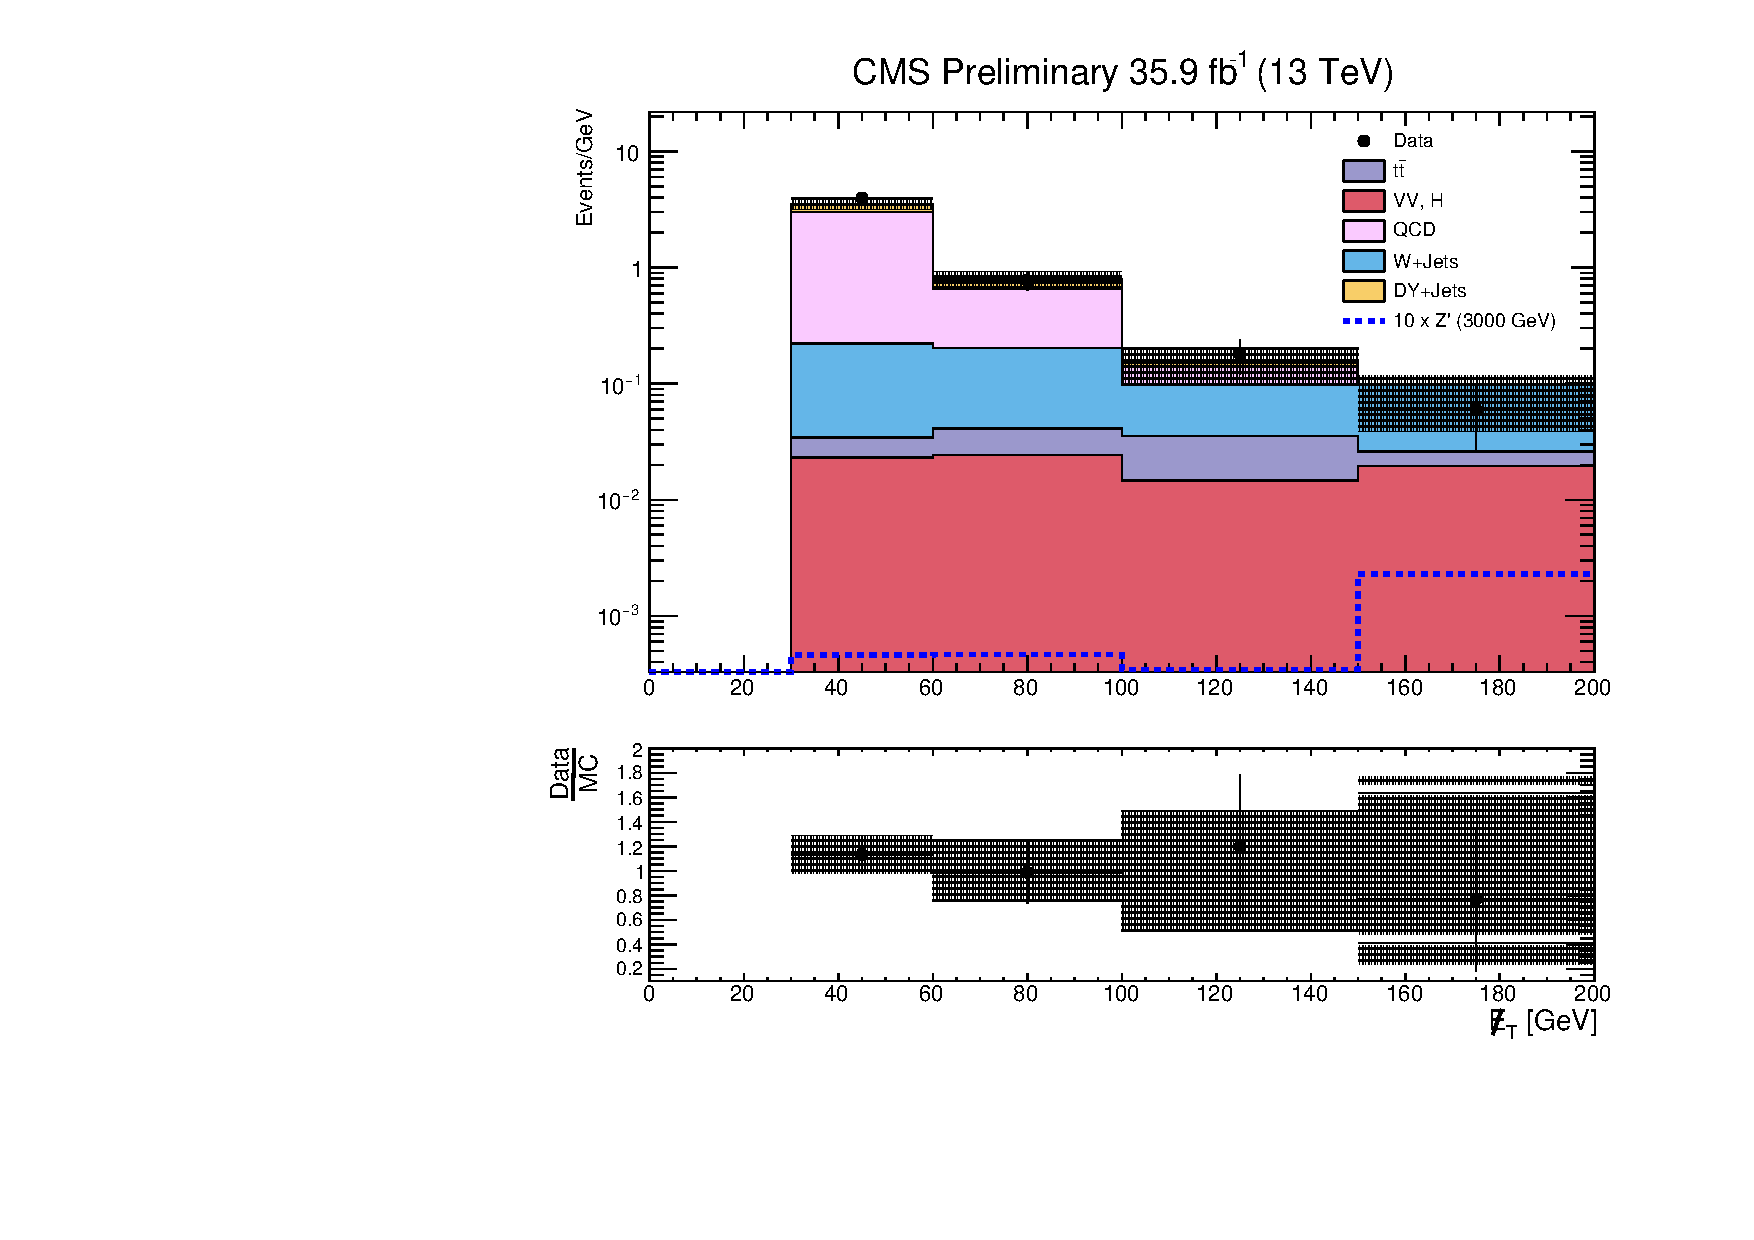
\includegraphics[clip,width=0.46\textwidth]{figuras/Chapter5/Plots_CosDphiInv/MET.pdf}
 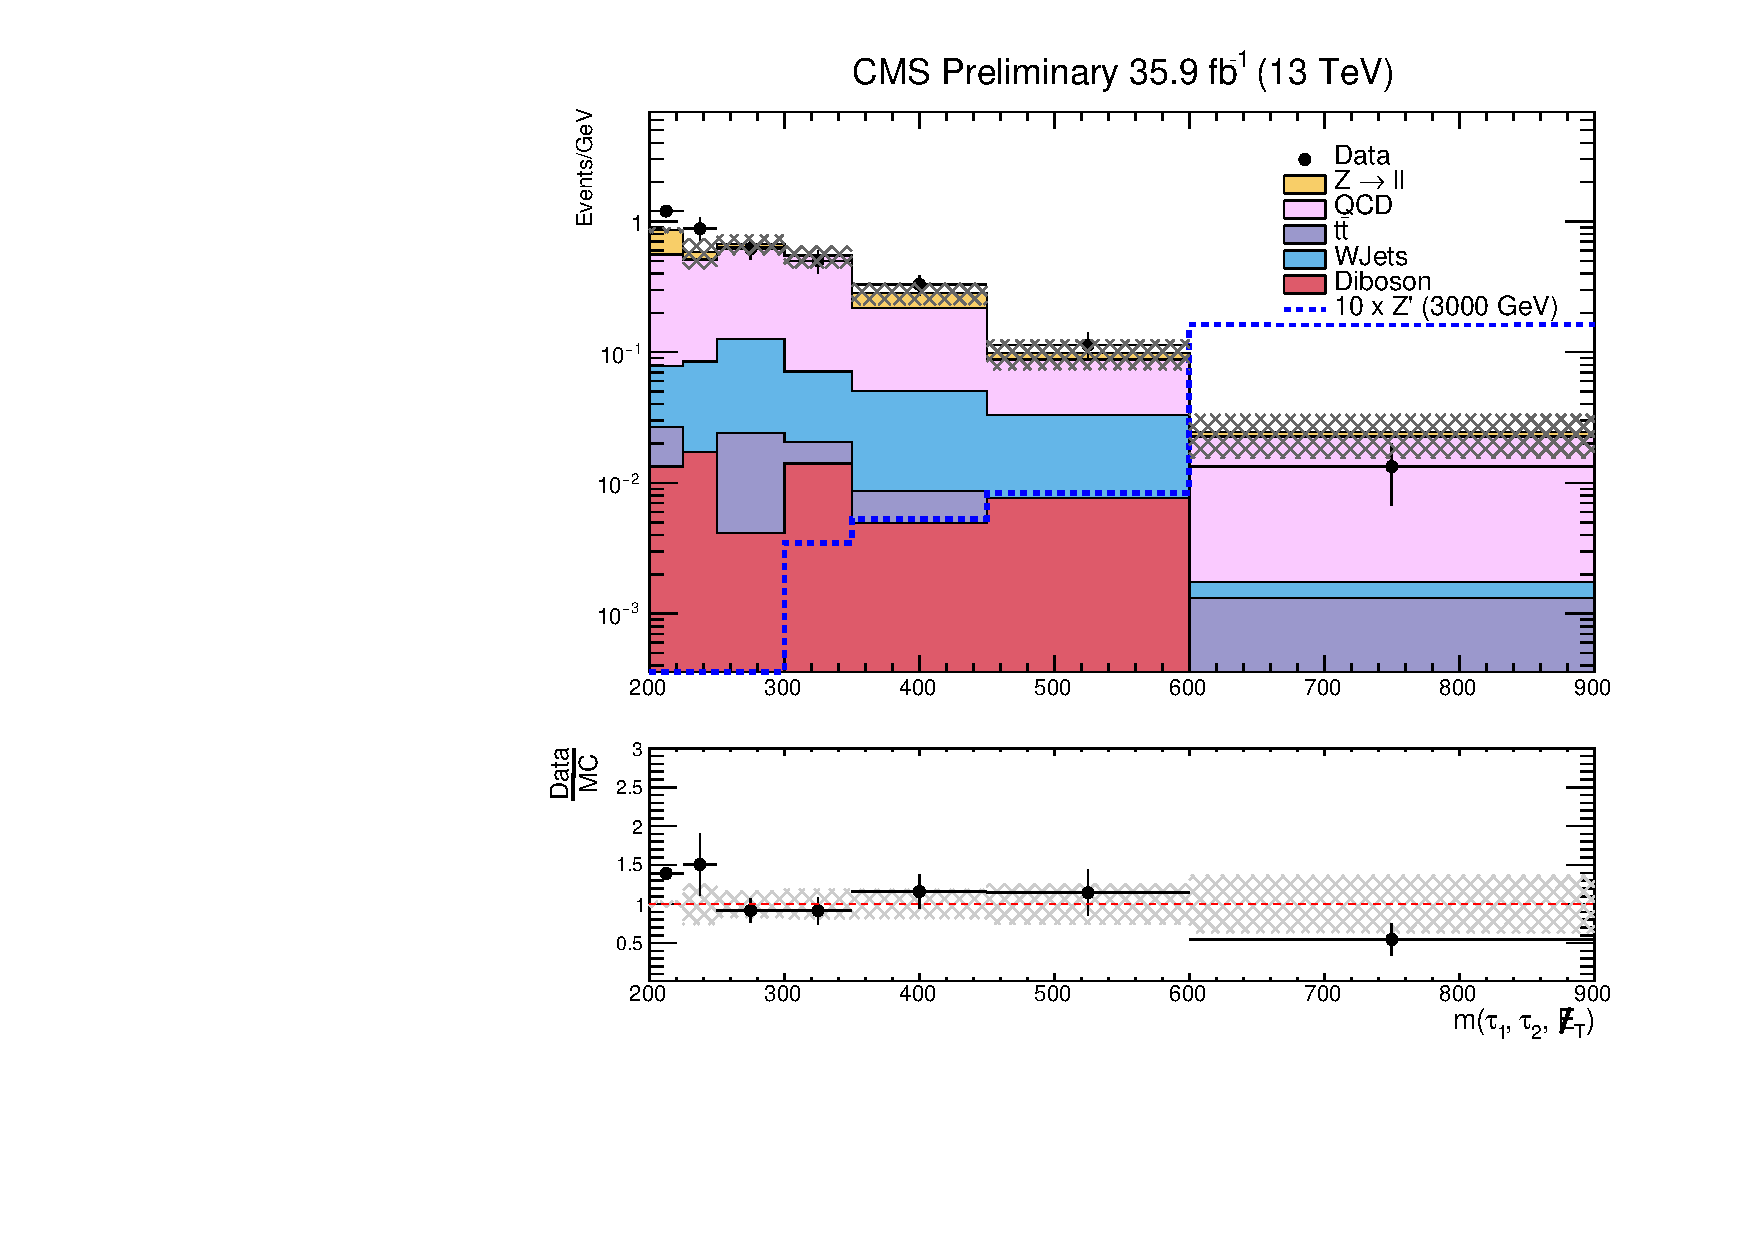
\includegraphics[clip,width=0.46\textwidth]{figuras/Chapter5/Plots_CosDphiInv/Mass.pdf}\hfill
 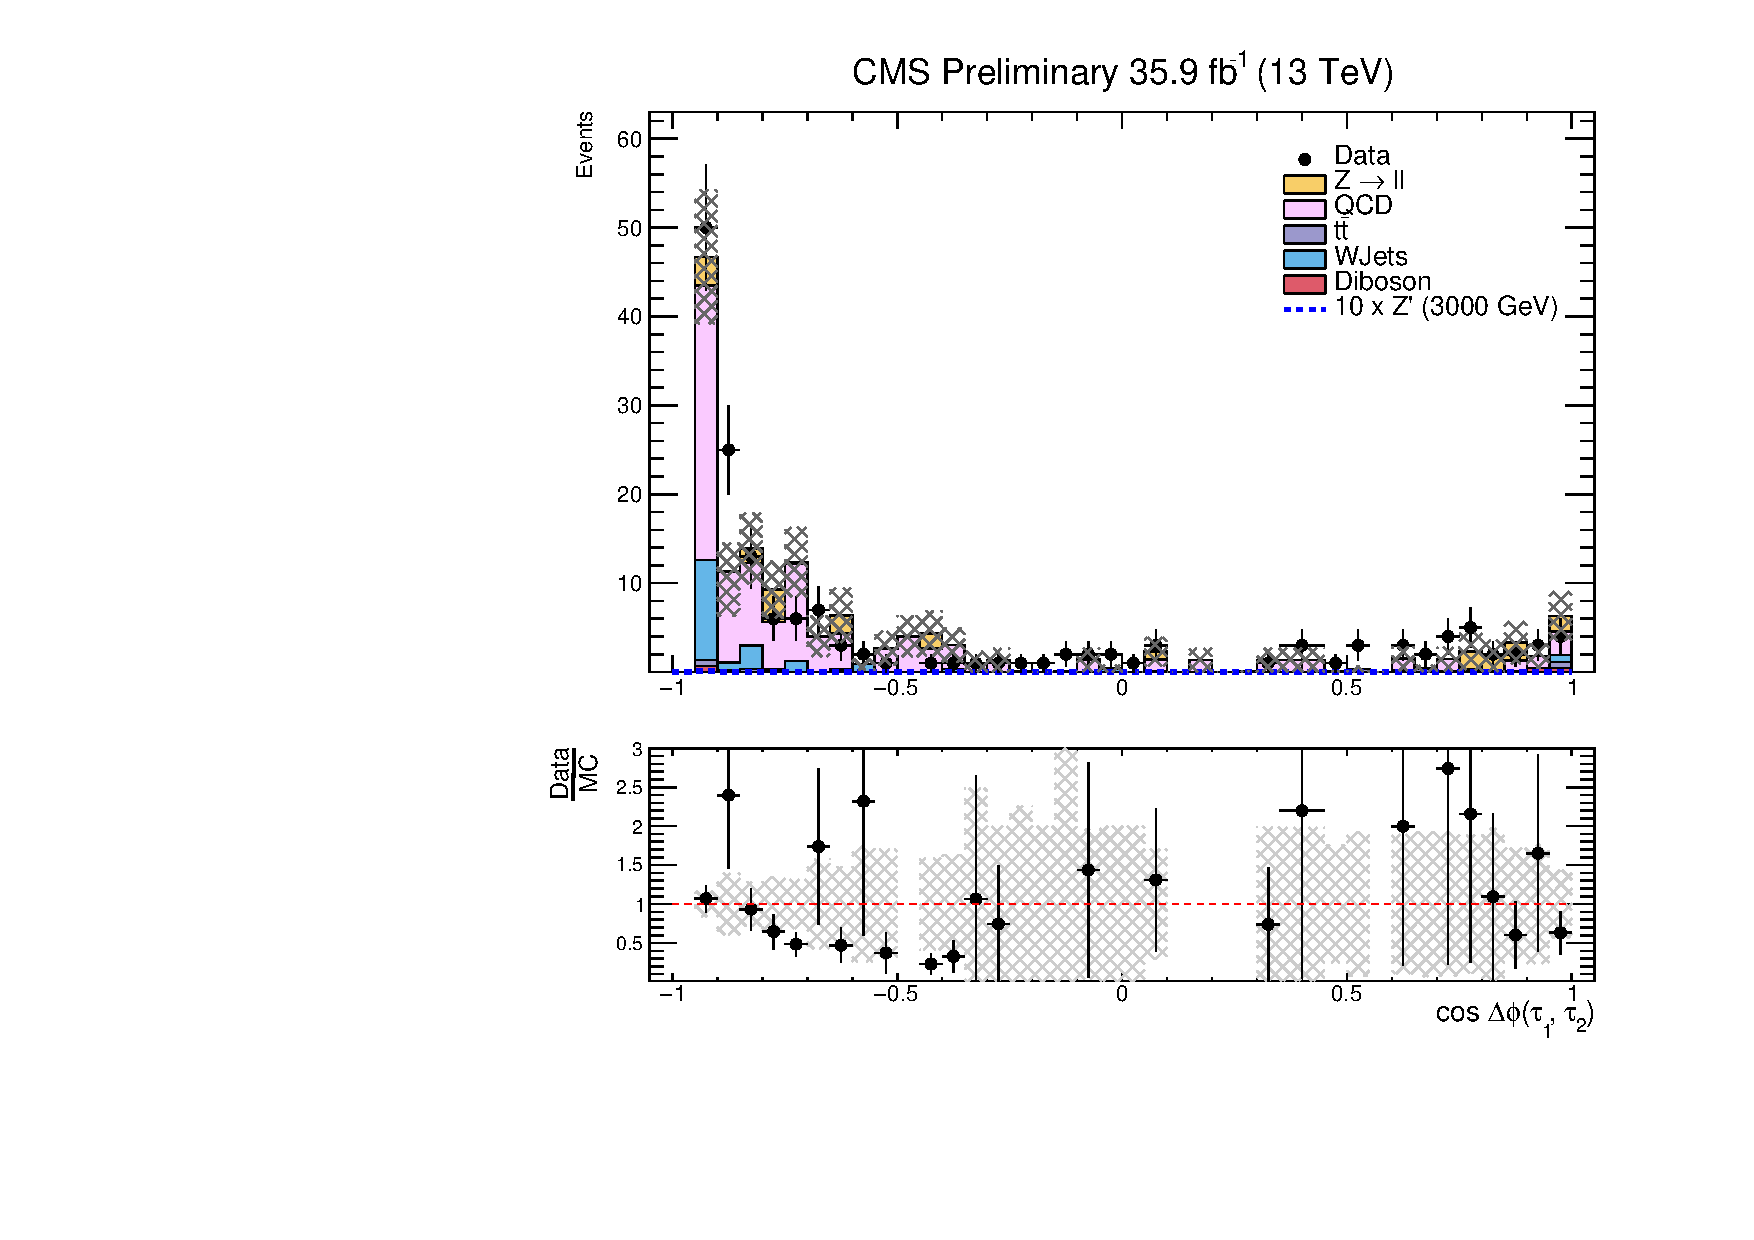
\includegraphics[clip,width=0.46\textwidth]{figuras/Chapter5/Plots_CosDphiInv/cosDphi.pdf}
 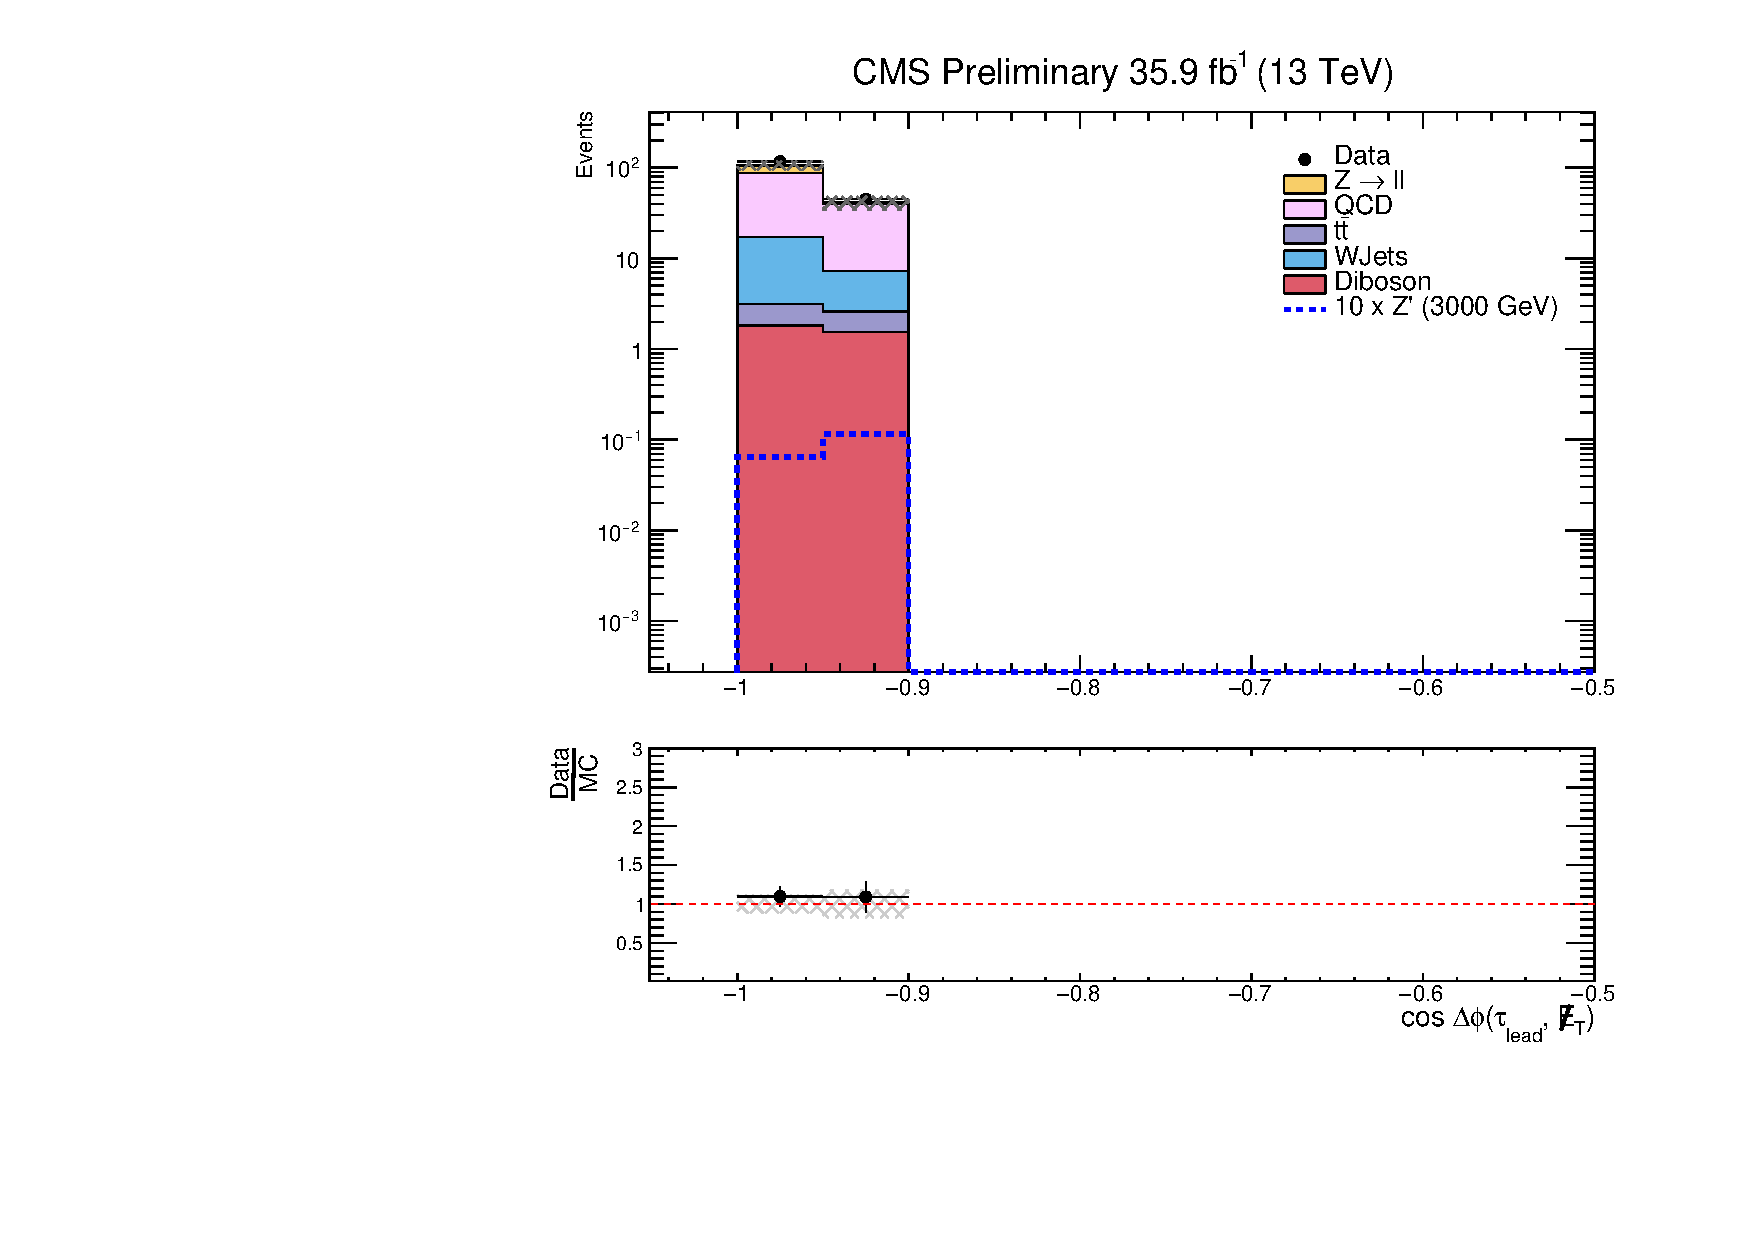
\includegraphics[clip,width=0.46\textwidth]{figuras/Chapter5/Plots_CosDphiInv/cosDphiTauMET.pdf} \hfill
 \end{center}
 \caption{Distribution of variables after applying the signal selection criteria but inverting
 the $\cos\Delta \phi (\tau_{1},\tau_{2})$ requirement. QCD background was estimated 
 using the data-driven method, while other backgrounds were estimated  directly 
 from simulated samples. The uncertainty is based on statistics. \pt~of the leading tau (top left),
 \pt~of the second tau (top right), \MET~(middle left), \mass~(middle right), 
 $\cos\Delta \phi (\tau_{1},\tau_{2})$ (bottom left) and $\Delta \phi (\tau_{lead}, \not\!\!E_T)$ (bottom right).}
\label{fig:cosDphiInv}
 \end{figure}

 
\noindent where $P_{MC}(n)$ is the probability to 
obtain $n$ interactions in the simulated event. The pileup weights 
were applied using the certified JSON file (minimum bias 
cross-section of 69.2 mb).\\

\textbf{Corrections of tau identification and triggering} \\

\noindent The efficiency of the tau identification algorithm 
must be taken into account when the expected 
simulated events are estimated. A comparison 
between data and SM processes is used in order 
to obtain the Data/MC tau identification scale factor (TauID. SF)
to correct the MC prediction; such comparison is performed using 
Z and W events, that decay into taus. The TauID SF depends on the 
isolation working point. Since in this analysis the Tight WP was used,
the TauID. SF applied for a single hadronic tau is 0.95 
\cite{CMS-PAS-TAU-16-002}; in consequence, the overall scale factor,
due to the identification of two hadronic taus, that was 
applied was 0.90$\sim$0.95$\times$0.95.\\

\noindent As mentioned in section \ref{sec:TriggerSelection}, the trigger
was not applied on MC samples due to the difficulty of modeling 
it in simulation. Instead, its efficiency was measured from the data 
and used in the simulated events as a weight, which is dependent on 
the $\tau$-\pt. The  applied trigger weight, per hadronic tau,
is described by equation \ref{eq:triggerEff}. \\

\noindent Note that the TauID. SF and the trigger weight were 
estimated per hadronic tau, and their data/MC agreement
for di-tau final states were validated simultaneously 
using the Drell-Yan control region (Figure \ref{fig:DYCR}).\\

\textbf{Recoil corrections} \\

\noindent The hadronic recoil for the Z and W bosons is not modeled properly
by the simulations and, therefore, recoil correction weights were applied. These
weights were computed from the difference between data and MC samples for a 
$Z\rightarrow\mu\mu$ control region, where no \MET~is expected 
in the event and, therefore, the four-vector of the Z boson can be 
determined accurately. The measured SFs are dependent on the 
transverse momentum of the boson involved in the process. These corrections
are only applied to the Drell-Yan and the W+Jets simulated samples.



\section{Systematic Uncertainties}
\label{sec:Systematics}

In order to confirm or discard the existence of a \Zprime~boson using 
the effective visible mass distribution, it is necessary 
to consider systematic uncertainties. These uncertainties can be 
caused by the finite resolution of the detector and the 
simulations involved in the analysis. There are two types of 
systematic uncertainties: the first type is related with the 
normalization of the distributions, for instance, the uncertainty 
in the luminosity measurement; while the second type is related 
the shape of the distributions, for instance, the uncertainties on 
the measurement of the variables need it to determine 
the \mass~distribution. \\

% simulation 
% the modeling of the simulation
% to measure physical variables such as the luminosity, the energy of the 
% particles, etc., and the modeling of the simulation, for example,
% the theoretical uncertainty on the cross-sections used to normalize
% the MC samples

\noindent The different sources of systematic uncertainties considered
in this analyses are:

\begin{itemize}
 \item Luminosity,
 \item Tau Identification,
 \item Tau Trigger,
 \item Tau Energy Scale,
 \item b-jet Identification,
 \item Jet Energy Scale,
 \item Missing Transverse Energy,
 \item Parton Distribution Functions,
 \item bin-by-bin statistical uncertainty.
 \item Background Estimations.
\end{itemize}

\textbf{Luminosity}\\

\noindent Since the luminosity is used to scale the simulated samples
(backgrounds and signal), the uncertainty on its measurement must be considered. The 
CMS Luminosity group has assigned a 2.5$\%$ uncertainty on the integrated luminosity of the 
data collected during 2016 \cite{Luminosity}.\\
 
\textbf{Tau Identification}\\

\noindent This uncertainty is associated to the tau 
tau identification algorithm. In this analysis, the HPS algorithm 
was used to identify taus. The efficiency can be 
affected by several factors such as: the efficiency
of the track finding algorithm; the efficiency of
identifying the tau decay mode; the probability of tracks associated 
to the underlying event, falling in the isolation cone; and
the probability of pions to fall outside the signal cone. The CMS group
dedicated to study the efficiency and reconstruction of 
the hadronic tau (Tau Particle Object Group, TauPOG) measured 
the overall systematic uncertainty and assigned to 
it a value of 5$\%$ (see Ref. \cite{TauPOG}). Since in this analysis
there are two correlated taus in the final state, an overall uncertainty 
of 10$\%$ was assigned on the simulated samples due to 
the di-tau identification. The TauPOG included an additional
uncertainty related to the high-\pt~tau identification efficiency, which 
affects the sensitivity of this analysis. This is an asymmetric 
uncertainty assigned per hadronic tau, which depends on its momentum; 
the uncertainty on the tau identification goes from $-35\%$ up to $5\%$ of 
the tau momentum (see Ref. \cite{TauPOG}); this result in an uncertainty 
of the order of 10$\%$ for masses around 500 \GeV~and of the order of 25$\%$ 
for masses around 2 \TeV. The uncertainty on the high-\pt~tau identification 
affects the shape of the \mass~distribution; this is determined by 
applying the \pt~dependent weights, per tau, and extracting 
varied mass templates, which are included as shape systematics.\\

\textbf{Tau Trigger}\\

\noindent Another source of uncertainty comes from the modeling
of the tau trigger at simulation level (see 
Section \ref{subsec:TriggerEff}). In order to model 
the trigger for each hadronic tau, weights were 
calculated using the tag-and-probe method. Due to the inefficiency observed for taus 
whose \pt~is greater than 70 \GeV, a systematic uncertainty of 5$\%$ is assigned per 
hadronic tau. The overall trigger uncertainty, when considering both taus, is 10$\%$.\\

% are fully 
% correlated, i.e., if the trigger uncertainty per tau is 5$\%$, then the total uncertainty 
% for the di-tau final state is 10$\%$ (2 $\cdot$ 5$\%$). \\

\textbf{The Tau Energy Scale}\\

\noindent The tau energy scale is calculated, using
simulated data, as the ratio between the energy of the reconstructed tau
and the energy of the visible decay products of the generated tau.
It represents the detector response to the hadronic tau. The precise 
measurement of the 4-momentum of the tau decay 
components is important for this analysis since the effective visible mass is computed from them
and from the missing transverse energy. There are systematic uncertainties 
inherent to the experimental identification of taus, that must be considered 
in the final result of the analysis. There are two sources of uncertainty: 
the first one comes from the measurement of energy clusters and 
the track reconstruction of the individual tau decay products; the second one 
comes from the fact that it is not possible to know whether all the tau visible 
decay products were included or not (for example, neutral pions which 
can fall outside the signal cone). Studies performed by the TauPOG conclude that 
no corrections must be applied on the tau energy measurement and that 
an overall tau energy scale uncertainty of 3$\%$, independently of the
tau decay mode, must be applied \cite{TauPOG}. This systematic effect
results in a 3$\%$ uncertainty in the signal yield and up to $\sim$11$\%$
in the background yields.\\

% This uncertainty is included 
%  as a shape uncertainty since the \mass~distribution depends on the tau energy.\\

\textbf{b-jet Identification}\\

\noindent Another source of uncertainty comes from the b-tagging
b-tagging identification algorithm used in this analysis. A 30$\%$ uncertainty on the 
b-jet mis-tagging rate was measured by the CMS b-tagging group (see Ref. \cite{bjetID}). Since in this
analysis there was a b-jet veto, this uncertainty must be taken into account. This was done 
using the equation:

\begin{equation}
\epsilon^{N\ b-tag \ < \ 1} = 1 - \sum_{n = 1} P(n) \cdot \sum_{m=1}^{n} \cdot C(n,m) \cdot f^{m} \cdot (1-f)^{n-m} \; , 
\end{equation}

\noindent where the second term on the right side represents 
the efficiency of identifying at least one b-jet in the event, $n$ is the number 
of jets, $P(n)$ is the probability to obtain $n$ jets in a event, $f$ is the 
probability that a jet can be misidentified as a b-jet and $C(n,m)$ are
the combinatorial factors. The systematic uncertainty due to the b-jet veto 
requirement was estimated, using the equation, considering the misidentification rate at the 
Loose CSVv2 working point (measured by the CMS b-tagging group) together with
the probability to obtain at least one b-jet in an event ($\sim$10$\%$). The resulting 
uncertainty is $\sim5\%$ on the signal samples is $\sim5\%$. The same uncertainty is 
assigned to the background samples where b-jets are not expected in the event, such as Drell-Yan 
and DiBoson samples. For backgrounds such as W+Jets, where at least one 
real jet is expected, and \ttbar, where b-jets are expected, this uncertainty is 10$\%$. \\
% 
% This correction has a very minor effect on the spectrum of the total transverse mass and
% hence is taken into account as an normalization uncertainty.

\textbf{Jet Energy Scale}\\

\noindent The jet reconstruction and, in consequence, its energy measurement have many 
sources of uncertainties such as the non-linear calorimeter response, the pileup 
interactions, the underling event, the electronic noise, etc. Therefore,
corrections are applied on the jet reconstruction, known as Jet Energy 
Corrections (JEC), to account for all these effects, allowing
an improved match between the MC predictions and the data (see section \ref{sec:Jet}). The 
Jet  Energy Scale (JES) corrections are part of the JEC. As recommended by 
the CMS JetMET POG, a 3$\%$ or 5$\%$ uncertainty (depending on 
the $\eta$ and \pt~of the jet) must be included in order to take into account
these systematic effects \cite{JetMETPOG}. This uncertainty makes the 
signal and MC based backgrounds fluctuate up to $\sim$12$\%$. \\

\textbf{Missing Transverse Energy}\\

\noindent Since the \MET~is inferred from the 4-momenta of all the 
reconstructed final states in the event, its systematic 
uncertainty depends on the topology of the signal process.
The uncertainty due to the \MET~on the signal 
acceptance depends mainly on the tau energy scale (TES),
the jet energy scale (JES) and the unclustered energy (UCE). The 
uncertainty on the UCE is 10$\%$, as recommended by the 
CMS JetMET POG. Considering the uncertainties coming from UCE, TES and JES, one 
gets a systematic uncertainty of 0.5$\%$ due to the \MET~on the 
simulated background yields.\\

\textbf{Parton Distribution Functions}\\

\noindent Another source of systematic uncertainty on the MC samples comes from the imprecise
knowledge of the parton distribution functions (PDF) used in the event simulation. These
uncertainties were estimated following the Run II recommendations given by the LHC 
group dedicated to study the PDFs \cite{PDFUncertainty}. These uncertainties
were estimated with the 68$\%$ confidence level using the ``PDF4LHC15\_mc'' sets
of PDFs. As a result, the PDF uncertainties for the MC samples used in this 
analysis are smaller than their bin-by-bin statistical uncertainties and, therefore,
they are negligible for the MC background samples. In the case of the 
signal, the PDF uncertainties varies from 0.7$\%$ for the \Zprime~sample with a mass 
of 500 \GeV~up to 12$\%$ for the \Zprime~sample with a mass of 3 \TeV. \\

 \textbf{bin-by-bin statistical uncertainty}\\
 
 \noindent The finite statistics of the simulated samples
 must be included as an additional uncertainty. With this purpose, 
 a per-bin uncertainty is estimated by changing the yield of given bin, within 
 its statistical uncertainty, while keeping the yields of the other bins unchanged, and 
 evaluating its effect on the shape of the \mass~distribution.\\
 
%  This uncertainty is known as bin-by-bin statistical uncertainty.

 \textbf{Background Estimations}\\

\noindent As described in section \ref{subsec:QCD}, the QCD background contamination
was estimated using a data-driven method. Since, in order to estimate and subtract
this background, simulated samples are used, the systematic effects on the MC samples mentioned 
above must be considered. With this purpose, these uncertainties are propagated 
throughout the subtraction.\\

% in order to compute the uncertainty on the QCD background prediction
% 
% estimate the QCD background in 
% 
% the background simulated samples were subtracted from the data n order 
% the control regions, the systematic effects on the MC samples, mentioned 
% above, must be considered to compute the systematic uncertainty on the QCD 
% background prediction;  

\noindent Besides, a systematic uncertainty is assigned on the QCD estimation due to 
the measurement of the $OS/LS$ transfer factor used to derive the contamination 
of this background in the signal region. Since the measured $OS/LS$ ratio 
is 1.34 $\pm$ 0.12, a relative uncertainty of 9$\%$ is considered on 
the QCD background estimation. In the case of the Drell-Yan 
background, an uncertainty of 8$\%$ is assigned due to the effect of the 
ratio between the data and the expected background measured in the Drell-Yan 
control region (see section \ref{subsec:DY}). In the case of the diBoson background, it is
not possible to obtain a semi-clean enriched sample using the di-hadronic final state, due to the high 
QCD contamination; therefore, this sample was defined using the 
\Zprimetoemu~channel. As a result, the data$/$MC scale factor obtained 
was 1.01 $\pm$ 0.20 and, consequently, a 20$\%$ systematic uncertainty was assigned
on diBoson background \cite{ZaixingThesis}. These systematic uncertainties,
due to the measurement of data$/$MC scale factors or the measurement of 
transfer factors, are known as closure and normalization uncertainties. In the case of 
W+Jets and \ttbar~backgrounds, these sources of uncertainty are not considered since 
no scale factors nor transfer factors were used for their estimation. \\

\textbf{Summary of the applied systematic uncertainties}\\

\noindent Table \ref{table:SystematicsTable} shows the values of systematic
uncertainties considered for the signal and backgrounds used in this analysis. The most 
important source of systematic uncertainty is the high-\pt~tau identification which, as 
mentioned above, corresponds to 25$\%$ uncertainty in the case of a reconstructed 
effective visible mass of 2 \TeV, affecting considerably the sensitivity of the search.

\begin{table}[ht]
\begin{center}
 \begin{tabular}{|l|c|c|c|c|c|c|} \hline \hline                                                                                                                                         
 Source                           &  QCD &  DY  & W+Jets & \ttbar &  DiBoson  & Signal \\                 
   \hline Lumi                    & --   &   L  &    L   &    L   &   L  &   L    \\                                                                       
   \hline $\tau_{h}$ Trig         & --   &  10  &   10   &   10   &  10  &  10    \\                                                                       
   \hline $\tau_{h}$ ID           & --   &  10  &   10   &   10   &  10  &  10    \\
   \hline high-\pt~$\tau_{h}$ ID  & --   &   s  &    s   &    s   &   s  &   s    \\                                                                       
   \hline TES                     & --   &  11  &   11   &   11   &   8  &   3    \\                                                                       
   \hline b ID                    & --   &   5  &   10   &   10   &   5  &   5    \\                                                                       
   \hline JES                     & --   &   8  &   12   &   12   &   8  &   2    \\                                                                        
   \hline pdf                     & --   &  --  &   --   &   --   &  --  & (1-12) \\                                                                       
   \hline bin-by-bin stat.        & s    &   s  &    s   &    s   &   s  &   s    \\                                                                       
   \hline Closure+Norm.           & 9    &   8  &   --   &   --   &  20  &        \\                                                                       
   \hline \hline                                                                                                                                                                        
 \end{tabular}                                                                                                                                                                           
 \caption{Summary of systematic uncertainties. Values are given in                                                                                                                      
   percent.  ``s'' indicates template variations (``shape''                                                                                                                             
   uncertainties). $\rm L=2.5\%$.}                                                                                                                                                      
 \label{table:SystematicsTable}                                                                                                                                                         
 \end{center}
\end{table} 

\section{Summary}
\label{Summary}

All the features involved in the search for \Zprime~bosons in the di-hadronic tau final 
channel were presented in this chapter. The trigger selection for two-hadronic taus events
was described in section \ref{sec:TriggerSelection}. The data collected by the CMS experiment 
from the pp collisions at \sqrts~13 \TeV, delivered by the LHC during 2016, along with
the simulated samples used for this search, were presented in section \ref{sec:Samples}. The event selection 
carried out to optimize the signal selection and to reduce any background 
contribution, minimizing the systematic uncertainties, was outlined in 
section \ref{sec:EventSelection}. The background estimation in the signal region (Section \ref{sec:BackgroundEstimation}), 
considering the corrections on the simulated samples, was performed and was validated using the 
N-1 distributions (section \ref{subsec:ValidationSignalSelections}) and the inverted 
$\cos \Delta\phi(\tau_{h},\tau_{h})$ control region (section \ref{subsec:Validation}). Finally, all the systematic
uncertainties that affect the signal and background estimations are listed in section \ref{sec:Systematics}.
As a result, the estimations of the backgrounds and of the expected signal are 
reliable (Table \ref{tab:signalregion}) and, therefore, any excess observed in the 
\mass~distribution (Figure \ref{fig:SR_Result}), with real data, would represent an evidence of 
the existence of a \Zprime~boson. In the next chapter, the complete analysis, 
assuming the nonexistence of a \Zprime~boson is presented and exclusion limits are estimated.


% the search perform with the 2016 data
% is presented. 
% presented the performed statistical analysis,
% assuming the nonexistence of a \Zprime~boson and, consequently, exclusion limits 
% are estimated considering the involved systematic uncertainties. Additional to the final 
% results, conclusions on the search for \Zprime~bosons in the di-hadronic tau final state
% using 2016 data are presented in the following chapter.
% 


